\documentclass[a4paper]{article}
\usepackage[utf8]{inputenc}
\usepackage{vntex}
\usepackage{a4wide,amssymb,epsfig,latexsym,multicol,array,hhline,fancyhdr}
\usepackage{booktabs}
\usepackage{amsmath}
\usepackage{lastpage}
\usepackage{enumerate}
\usepackage{color}
\usepackage{graphicx}
\usepackage{array}
\usepackage{tabularx}
\usepackage[justification=centering, font=small, labelfont=bf]{caption}
\usepackage{multirow}
\usepackage{rotating}
\usepackage{geometry}
\usepackage{setspace}
\usepackage{tikz}
\usepackage{float}
\usepackage{listings}
\usepackage{url}
\usetikzlibrary{arrows,arrows.meta,shapes.geometric,shapes.misc,positioning,fit,calc}
\usepackage{hyperref}
\hypersetup{urlcolor=blue,linkcolor=blue,citecolor=black,colorlinks=true}

\def\UrlBreaks{\do\/\do-\do_}

\geometry{
    a4paper,
    left=20mm,
    right=20mm,
    top=25mm,
    bottom=25mm
}

\captionsetup{justification=centering}

\setlength{\headheight}{40pt}
\pagestyle{fancy}
\fancyhead{}
\fancyhead[L]{
 \begin{tabular}{rl}
    \begin{picture}(25,15)(0,0)
    \put(0,-8){
\includegraphics[width=8mm, height=8mm]{logoITSGUsmall.png}}
   \end{picture}&
	\begin{tabular}{l}
		\textbf{\bf \ttfamily Trường Đại học Sài Gòn}\\
		\textbf{\bf \ttfamily Khoa Công Nghệ Thông Tin}
	\end{tabular} 	
 \end{tabular}
}
\fancyhead[R]{
	\begin{tabular}{r}
		\scriptsize \bf \ttfamily ĐỒ ÁN CÔNG NGHỆ PHẦN MỀM \\
		\scriptsize \bf \ttfamily ASSIGNMENT 2 -- NHÓM 16: BREWLITE
	\end{tabular}  
}
\fancyfoot{}
\fancyfoot[L]{\scriptsize \ttfamily Báo cáo Tổng kết Đồ án Nhóm 16 -- Hệ thống Cà phê BrewLite}
\fancyfoot[R]{\scriptsize \ttfamily Trang {\thepage}/\pageref{LastPage}}
\renewcommand{\headrulewidth}{0.3pt}
\renewcommand{\footrulewidth}{0.3pt}

\lstset{
  language=bash,
  basicstyle=\scriptsize\ttfamily,
  keywordstyle=\color{blue}\bfseries,
  commentstyle=\color{gray}\itshape,
  stringstyle=\color{red},
  numbers=left,
  numberstyle=\tiny\color{gray},
  stepnumber=1,
  numbersep=6pt,
  backgroundcolor=\color{white},
  showspaces=false,
  showstringspaces=false,
  showtabs=false,
  frame=single,
  tabsize=2,
  captionpos=b,
  breaklines=true,
  breakatwhitespace=false
}

\begin{document}

% ==================== TRANG BÌA ====================
\begin{titlepage}
\thispagestyle{empty}
\begin{singlespace}
\begin{center}
{\large \textbf{TRƯỜNG ĐẠI HỌC SÀI GÒN}} \\
{\large \textbf{KHOA CÔNG NGHỆ THÔNG TIN}} \\
\textbf{BỘ MÔN CÔNG NGHỆ PHẦN MỀM} \\
------o0o------
\end{center}

\vspace{0.3cm}
\begin{center}

\includegraphics[width=2.8cm]{logoITSGU.png}
\end{center}
\vspace{0.3cm}

\begin{center}
\begin{tabular}{c}
	\multicolumn{1}{l}{\textbf{{\Large BÀI TẬP LỚN: CÔNG NGHỆ PHẦN MỀM}}}\\
	\vspace{0.05cm}\\
	\hline
	\\
	\multicolumn{1}{l}{\textbf{{\large ASSIGNMENT 2: REQUIREMENTS TO DEPLOYMENT}}}\\
	\vspace{0.15cm}\\
	\textbf{{\LARGE HỆ THỐNG CÀ PHÊ BREWLITE}}\\
	\vspace{0.15cm}\\
	\textbf{{\Large BÁO CÁO TỔNG KẾT ĐỒ ÁN -- NHÓM 16}}\\
	\vspace{0.1cm}\\
	\textbf{{\normalsize Đề tài: Xây dựng Hệ thống Đặt cà phê PWA \& Quản lý Đơn hàng}}\
	\\
	\hline
\end{tabular}
\end{center}

\vspace{0.3cm}
\begin{center}
\textbf{GIẢNG VIÊN HƯỚNG DẪN: ThS. Từ Lãng Phiêu}
\end{center}
\vspace{0.2cm}

\begin{center}
\textbf{DANH SÁCH SINH VIÊN THỰC HIỆN (NHÓM 16):} \\[0.15cm]
\begin{tabular}{|c|>{\raggedright\arraybackslash}p{4.2cm}|c|>{\raggedright\arraybackslash}p{6.5cm}|}
\hline
\textbf{STT} & \textbf{Họ và Tên} & \textbf{MSSV} & \textbf{Màn hình \& Luồng Nghiệp vụ Đảm nhận} \\ \hline
1 & Trần Vĩnh Thọ Lân & 3124560049 & Màn hình \& Luồng Menu sản phẩm (PWA, Monorepo, CI/CD, E2E Test) \\ \hline
2 & Nguyễn Tuấn Khôi & 3124410190 & Màn hình \& Luồng Chi tiết món \& Tùy chọn (Size, Topping, Tính giá) \\ \hline
3 & Phan Vũ Việt Quang & 3124560072 & Màn hình \& Luồng Giỏ hàng, Đặt đơn \& Thanh toán Idempotency \\ \hline
4 & Nguyễn Hữu Chí Công & 3124720010 & Màn hình \& Luồng Đăng nhập, Đăng ký (JWT Auth, Bcrypt, Docker) \\ \hline
\end{tabular}
\end{center}

\vspace{0.4cm}
\begin{center}
\textbf{HỌC KỲ: I -- NĂM HỌC 2026--2027} \\[0.1cm]
\textbf{TP. HỒ CHÍ MINH, THÁNG 11/2026}
\end{center}

\end{singlespace}
\end{titlepage}

\newpage
\tableofcontents
\newpage

% ==================== MỤC 1: BỐI CẢNH & PHẠM VI ====================
\section{Bối cảnh Đề tài, 6 Stakeholders, Phân công \& Phạm vi Đồ án (Task 1.1)}

\subsection{Bối cảnh Thực tiễn Hệ thống Cà phê BrewLite}
Trong lĩnh vực kinh doanh dịch vụ ăn uống (F\&B) hiện đại, việc số hóa quy trình vận hành và tối ưu hóa trải nghiệm khách hàng tại cửa hàng đóng vai trò sống còn. Hệ thống cà phê \textbf{BrewLite} được Nhóm 16 thiết kế nhằm giải quyết bài toán ùn tắc cục bộ tại quầy thu ngân vào các khung giờ cao điểm (8h--9h sáng và 12h--13h trưa), đồng thời mang lại trải nghiệm gọi món mượt mà không độ trễ. 

Hệ thống được tổ chức thành 4 điểm chạm kỹ thuật số trọng tâm tương ứng với 4 phân hệ cốt lõi:
\begin{itemize}
    \item \textbf{Phân hệ Menu sản phẩm (Thành viên 1 -- Trần Vĩnh Thọ Lân):} Khách hàng quét mã QR tại bàn hoặc truy cập Web PWA để tải toàn bộ thực đơn phân cấp trong dưới 1.5 giây, hỗ trợ tìm kiếm tức thì theo từ khóa, lọc danh mục theo tabs và hiển thị nhãn hết hàng (Out of Stock).
    \item \textbf{Phân hệ Chi tiết món \& Tùy chọn (Thành viên 2 -- Nguyễn Tuấn Khôi):} Cung cấp trải nghiệm tùy biến sâu với kích cỡ (Size S/M/L) và danh sách Topping đa dạng; áp dụng công thức tính giá động phản hồi theo thời gian thực (Real-time dynamic price calculation).
    \item \textbf{Phân hệ Giỏ hàng, Đặt đơn \& Thanh toán Idempotent (Thành viên 3 -- Phan Vũ Việt Quang):} Quản lý giỏ hàng phía Client qua reactive state Zustand, khởi tạo đơn hàng với cơ chế khóa lạc quan (Optimistic Locking) trên CSDL PostgreSQL, tích hợp cổng thanh toán giả lập với cơ chế chống trừ tiền trùng lặp tuyệt đối (Idempotency Key).
    \item \textbf{Phân hệ Đăng nhập, Đăng ký \& Hạ tầng Docker (Thành viên 4 -- Nguyễn Hữu Chí Công):} Bảo mật mật khẩu với mã hóa Bcrypt một chiều (Salt Rounds = 10), phát hành và xác thực phiên làm việc phi trạng thái bằng JSON Web Token (JWT), phân quyền vai trò (RBAC) và đóng gói triển khai monorepo đồng bộ qua Docker Compose 3 containers.
\end{itemize}

\subsection{Bảng Phân công Trách nhiệm 4 Thành viên (Nhóm 16)}
Bảng~\ref{tab:phan_cong_nhom} định vị rõ ràng trách nhiệm chuyên môn của 4 thành viên thuộc Nhóm 16:

\begin{table}[H]
\centering
\small
\begin{tabular}{|c|>{\raggedright\arraybackslash}p{3.2cm}|>{\raggedright\arraybackslash}p{3.8cm}|>{\raggedright\arraybackslash}p{6.8cm}|}
\hline
\textbf{STT} & \textbf{Thành viên} & \textbf{Phân hệ / Luồng} & \textbf{Nhiệm vụ \& Hiện thực Kỹ thuật Đảm nhận} \\ \hline
1 & \textbf{Trần Vĩnh Thọ Lân} \newline (Thành viên 1) & Menu sản phẩm (PWA \& API) & Khởi tạo Monorepo Turborepo, Task 1.1 Context \& Scope, 6 Stakeholders, Ma trận rủi ro, 5 sơ đồ UML Menu, Code Web PWA \texttt{page.tsx}, API NestJS \texttt{products/}, CI/CD GitHub Actions, E2E Test. \\ \hline
2 & \textbf{Nguyễn Tuấn Khôi} \newline (Thành viên 2) & Chi tiết món \& Tùy chọn (Size/Topping) & Task 1.2 SRS FR-03, 4 Quy tắc nghiệp vụ BR-01..BR-04, Công thức tính giá động, 5 sơ đồ UML Chi tiết món, Modal \texttt{ProductDetailModal.tsx}, API \texttt{GET /products/:id}, 13 Unit Tests (100\%). \\ \hline
3 & \textbf{Phan Vũ Việt Quang} \newline (Thành viên 3) & Giỏ hàng, Đặt đơn \& Thanh toán & Task 1.3 Bảng đặc tả Use-Case trọng tâm "Đặt và thanh toán đơn hàng", Đặc tả FR-04, 10 sơ đồ UML Giỏ hàng \& Thanh toán, Code State \texttt{cartStore.ts}, API \texttt{POST /orders} (DB Transaction), API \texttt{POST /payments} (Idempotency Key). \\ \hline
4 & \textbf{Nguyễn Hữu Chí Công} \newline (Thành viên 4) & Đăng nhập/Đăng ký (JWT) \& Docker & Task 1.2 NFR Bảo mật JWT \& Bcrypt (Salt=10), FR-08, 5 sơ đồ UML Auth, Giao diện \texttt{AuthModal.tsx}, Backend API \texttt{auth.service.ts}, \texttt{JwtAuthGuard}, Đóng gói Docker Compose 3 containers, Unit test Auth. \\ \hline
\end{tabular}
\caption{Bảng phân công trách nhiệm 4 thành viên thuộc Nhóm 16}
\label{tab:phan_cong_nhom}
\end{table}

\subsection{Bảng Phân tích 6 Nhóm Stakeholders Trọng tâm}
Theo chuẩn kỹ thuật phần mềm, 6 nhóm đối tượng liên quan trực tiếp đến hệ thống BrewLite được phân tích tại Bảng~\ref{tab:stakeholders}:

\begin{table}[H]
\centering
\small
\begin{tabular}{|c|>{\raggedright\arraybackslash}p{2.6cm}|>{\raggedright\arraybackslash}p{3.8cm}|>{\raggedright\arraybackslash}p{7.2cm}|}
\hline
\textbf{STT} & \textbf{Stakeholder} & \textbf{Mục tiêu chính (Goals)} & \textbf{Kỳ vọng \& Tiêu chí chấp nhận} \\ \hline
1 & \textbf{Khách hàng (Customer)} & Đặt đồ uống nhanh chóng, không phải xếp hàng chờ, xem rõ giá cả minh bạch. & Giao diện tải nhanh ($<1.5$s), tự tính giá khi đổi size/topping, thanh toán điện tử an toàn, nhận mã lấy đồ \texttt{\#ORD-XXXXXX} rõ ràng. \\ \hline
2 & \textbf{Nhân viên quầy (Barista)} & Tiếp nhận danh sách order chuẩn xác, hạn chế trao đổi miệng gây sai lệch. & Thông tin size, topping hiển thị chuẩn xác; trạng thái đơn chuyển đổi đúng quy trình: \texttt{PAID} $\rightarrow$ \texttt{PREPARING} $\rightarrow$ \texttt{READY} $\rightarrow$ \texttt{COMPLETED}. \\ \hline
3 & \textbf{Quản lý / PO} & Tối ưu hóa năng suất phục vụ, giảm thất thoát doanh thu, kiểm soát tồn kho. & Hệ thống ổn định, không overselling khi nhiều khách đặt cùng lúc; bàn giao sản phẩm theo Sprint đúng cam kết (DoD). \\ \hline
4 & \textbf{Giảng viên nghiệm thu} & Đánh giá năng lực kỹ thuật phần mềm, quy trình Agile Scrum, UML, CI/CD. & Tuân thủ quy tắc tuần tự 5 Task; sơ đồ UML chuẩn xác; source code monorepo có automated test; có URL Production qua HTTPS. \\ \hline
5 & \textbf{Nhóm sinh viên phát triển (Nhóm 16)} & Hiện thực trọn vẹn đồ án theo chuẩn SE, đạt điểm tối đa đồ án. & Phân chia công việc rõ ràng theo các luồng module cốt lõi; kiến trúc tách bạch; có ma trận truy vết đầy đủ từ yêu cầu đến test. \\ \hline
6 & \textbf{Đơn vị thanh toán (Mock)} & Bảo đảm tính toàn vẹn và an toàn của các giao dịch điện tử. & Xử lý giao dịch Idempotent qua \texttt{Idempotency-Key}, chống trừ tiền trùng lặp, trả về mã giao dịch tức thời. \\ \hline
\end{tabular}
\caption{Bảng phân tích 6 nhóm bên liên quan (Stakeholders) trong đồ án BrewLite}
\label{tab:stakeholders}
\end{table}

\subsection{Ranh giới Phạm vi Hệ thống (System Scope)}
\begin{itemize}
    \item \textbf{In-Scope (Giai đoạn 1 -- Cốt lõi đồ án):}
    \begin{enumerate}
        \item Xem thực đơn đồ uống phân cấp, tìm kiếm tức thì theo tên món và lọc theo tab danh mục.
        \item Xem chi tiết món trong modal, chọn kích cỡ (S/M/L) và topping, tính giá tự động theo thời gian thực.
        \item Quản lý giỏ hàng cục bộ (thêm, cập nhật số lượng, xóa món) với reactive state Zustand.
        \item Khởi tạo đơn hàng an toàn, kiểm tra tồn kho và commit transaction trong CSDL PostgreSQL.
        \item Thanh toán điện tử giả lập không tiền mặt với cơ chế bảo vệ giao dịch Idempotent.
        \item Đăng ký tài khoản, đăng nhập xác thực JWT và mã hóa mật khẩu Bcrypt với salt rounds = 10.
        \item Tự động hóa kiểm thử đơn vị (Unit Tests), tích hợp liên tục (CI/CD GitHub Actions) và đóng gói Docker Compose.
    \end{enumerate}
    \item \textbf{Extended Scope (Giai đoạn 2 -- Tính năng mở rộng):} Tra cứu lịch sử đơn hàng của tài khoản, toast thông báo trạng thái đơn hàng thời gian thực.
    \item \textbf{Out-of-Scope (Bàn giao giai đoạn vận hành sau):} Tích hợp máy in hóa đơn nhiệt phần cứng tại quầy, đồng bộ POS đa chi nhánh vật lý, tích hợp webhook đối tác giao hàng bên thứ ba (GrabFood, ShopeeFood).
\end{itemize}

\subsection{Ma trận Đánh giá \& Kiểm soát Rủi ro Ban đầu}
Nhóm 16 đã phân tích và thiết lập các biện pháp kiểm soát rủi ro tại Bảng~\ref{tab:risks}:

\begin{table}[H]
\centering
\small
\begin{tabular}{|c|>{\raggedright\arraybackslash}p{2.6cm}|c|c|>{\raggedright\arraybackslash}p{6.8cm}|}
\hline
\textbf{Mã} & \textbf{Rủi ro Kỹ thuật} & \textbf{Mức độ} & \textbf{Tác động} & \textbf{Chiến lược Giảm thiểu Kỹ thuật} \\ \hline
\textbf{RSK-01} & Nghẽn mạng quầy giờ cao điểm & Cao & Nghiêm trọng & Xây dựng Web PWA nạp trước dữ liệu thực đơn, Next.js nạp dữ liệu tức thì dưới 1.5s, hỗ trợ hiển thị Loading Skeleton. \\ \hline
\textbf{RSK-02} & Tính toán sai lệch giá topping & Trung bình & Đáng kể & Tập trung hóa công thức tính giá: Client tính hiển thị tức thời, Backend NestJS kiểm tra và tính toán lại trước khi ghi đơn vào DB. \\ \hline
\textbf{RSK-03} & Trừ tiền trùng lặp (Double billing) & Cao & Nghiêm trọng & Triển khai cơ chế \texttt{Idempotency-Key} (UUIDv4) ở header API thanh toán, lưu hash kết quả giao dịch trong 24 giờ. \\ \hline
\textbf{RSK-04} & Rò rỉ mật khẩu và chiếm quyền & Cao & Nghiêm trọng & Băm mật khẩu bằng Bcrypt với Salt Rounds = 10; phát hành Access Token JWT thời hạn 15 phút, bảo vệ route bằng \texttt{JwtAuthGuard}. \\ \hline
\end{tabular}
\caption{Ma trận đánh giá và kiểm soát 4 rủi ro trọng tâm ban đầu}
\label{tab:risks}
\end{table}

\newpage
% ==================== MỤC 2: ĐẶC TẢ YÊU CẦU ====================
\section{Đặc tả Yêu cầu Phần mềm Toàn diện (SRS \& Use Cases -- Task 1.2 \& 1.3)}

\subsection{Danh mục Yêu cầu Chức năng (Functional Requirements -- FR)}
Toàn bộ 8 yêu cầu chức năng cốt lõi được chuẩn hóa theo chuẩn IEEE 830 tại Bảng~\ref{tab:srs}:

\begin{table}[H]
\centering
\small
\begin{tabular}{|c|>{\raggedright\arraybackslash}p{3.4cm}|c|>{\raggedright\arraybackslash}p{7.5cm}|}
\hline
\textbf{Mã FR} & \textbf{Tên chức năng} & \textbf{MoSCoW} & \textbf{Mô tả Nghiệp vụ \& Tiêu chí Chấp nhận} \\ \hline
\textbf{FR-01} & Duyệt thực đơn đồ uống & Must & Khách hàng quét mã QR hoặc mở Web PWA; tải danh mục và đồ uống dạng lưới card; hiển thị ảnh, tên, giá gốc, nhãn hết hàng. \\ \hline
\textbf{FR-02} & Lọc và tìm kiếm món & Must & Hỗ trợ tìm kiếm tức thời theo từ khóa tên món và thanh trượt tab danh mục (Cà phê phin, Espresso, Trà, Cold Brew). \\ \hline
\textbf{FR-03} & Chi tiết món \& Tùy chọn & Must & Mở Modal chi tiết món, cho phép chọn kích cỡ (S/M/L) và danh sách Topping; giá tự động nhảy theo công thức thời gian thực. \\ \hline
\textbf{FR-04} & Quản lý giỏ hàng & Must & Thêm món đã chọn size/topping vào giỏ, cập nhật số lượng, xóa món; tự động đồng bộ tổng tiền và hiển thị badge số lượng. \\ \hline
\textbf{FR-05} & Khởi tạo đơn hàng & Must & Xác nhận đơn hàng, gửi request \texttt{POST /orders}; kiểm tra tồn kho trong DB Transaction, sinh mã đơn hàng dạng \texttt{\#ORD-XXXXXX}. \\ \hline
\textbf{FR-06} & Thanh toán điện tử & Must & Thanh toán không tiền mặt (MoMo/VNPay/Thẻ); gửi header \texttt{Idempotency-Key} chống trừ tiền 2 lần khi mạng chập chờn. \\ \hline
\textbf{FR-07} & Xem mã đơn \& Biên lai & Must & Điều hướng đến màn hình xác nhận thành công; hiển thị mã \texttt{\#ORD-XXXXXX}, trạng thái \texttt{PAID}, danh sách món và mã QR nhận đồ. \\ \hline
\textbf{FR-08} & Đăng ký \& Đăng nhập JWT & Must & Đăng ký tài khoản với mật khẩu mã hóa Bcrypt (cost=10), đăng nhập nhận JWT Bearer Token, kiểm soát quyền truy cập \texttt{JwtAuthGuard}. \\ \hline
\end{tabular}
\caption{Bảng đặc tả 8 yêu cầu chức năng (FR) toàn hệ thống BrewLite}
\label{tab:srs}
\end{table}

\subsection{Quy tắc Nghiệp vụ \& Công thức Tính giá Tự động (Business Rules -- Thành viên 2)}
Phân hệ Chi tiết món do \textbf{Nguyễn Tuấn Khôi} phụ trách hiện thực các quy tắc nghiệp vụ (Business Rules) tính giá động:
\begin{itemize}
    \item \textbf{BR-01 (Kích cỡ đồ uống):} Mỗi sản phẩm có Size mặc định là Size S (không phụ thu, $+0$ VNĐ). Khách hàng có thể đổi sang Size M ($+6.000$ VNĐ) hoặc Size L ($+12.000$ VNĐ). Mỗi thời điểm chỉ được chọn duy nhất 1 kích cỡ.
    \item \textbf{BR-02 (Tùy chọn Topping):} Khách hàng có thể chọn nhiều Topping cùng lúc (Zero-to-Many). Giá của từng loại Topping được cộng dồn độc lập:
    \begin{itemize}
        \item Trân châu trắng: $+8.000$ VNĐ.
        \item Kem Cheese (Macchiato): $+10.000$ VNĐ.
        \item Thạch sương sáo: $+6.000$ VNĐ.
        \item Hạt sen tươi: $+10.000$ VNĐ.
    \end{itemize}
    \item \textbf{BR-03 (Công thức Tính Giá Động Toàn diện):} Giá thành tổng cộng của một món hàng được tính toán tức thời theo công thức KaTeX sau:
    \[
    \text{FinalPrice} = \left( \text{BasePrice} + \text{SizeAdjustment} \right) \times \text{Quantity} + \sum_{i=1}^{k} \left( \text{ToppingPrice}_i \times \text{Quantity} \right)
    \]
    \item \textbf{BR-04 (Xử lý Hết hàng):} Nếu một sản phẩm có trường \texttt{isAvailable = false} hoặc số lượng tồn kho bằng 0, giao diện hiển thị nhãn "Hết hàng" (Out of Stock Badge) và vô hiệu hóa nút "Thêm vào giỏ hàng" để ngăn ngừa tình trạng đặt vượt tồn kho thực tế.
\end{itemize}

\subsection{Đặc tả Chi tiết Luồng Nghiệp vụ Tạo Đơn hàng (FR-04 -- Thành viên 3)}
Bảng~\ref{tab:fr04_order} mô tả luồng nghiệp vụ tạo đơn hàng an toàn do \textbf{Phan Vũ Việt Quang} đặc tả:

\begin{table}[H]
\centering
\small
\begin{tabular}{|>{\raggedright\arraybackslash}p{3.4cm}|>{\raggedright\arraybackslash}p{12.2cm}|}
\hline
\textbf{Mã chức năng} & \textbf{FR-04: Quản lý Giỏ hàng và Tạo đơn hàng} \\ \hline
\textbf{Tác nhân (Actor)} & Khách hàng (Customer), Hệ thống CSDL (PostgreSQL) \\ \hline
\textbf{Mô tả tóm tắt} & Khách hàng quản lý giỏ hàng (thêm, sửa số lượng, xóa) và bấm tạo đơn hàng. Backend kiểm tra tồn kho, áp dụng khóa lạc quan và tạo đơn hàng trạng thái \texttt{PENDING}. \\ \hline
\textbf{Tiền điều kiện} & 1. Giỏ hàng có ít nhất một sản phẩm hợp lệ (\texttt{items.length >= 1}). \newline 2. Khách hàng đã đăng nhập tài khoản hợp lệ (JWT Token hợp lệ). \\ \hline
\textbf{Hậu điều kiện} & 1. Đơn hàng được tạo mới ở trạng thái \texttt{PENDING} với mã định danh \texttt{\#ORD-XXXXXX}. \newline 2. Tồn kho sản phẩm được cập nhật an toàn trong transaction CSDL. \newline 3. Chuyển tiếp khách hàng sang luồng thanh toán với mã \texttt{pendingOrderId}. \\ \hline
\textbf{Luồng sự kiện chính} & 
1. Khách hàng mở giỏ hàng, kiểm tra danh sách món đồ uống đã chọn. \newline
2. Khách hàng điều chỉnh số lượng hoặc áp dụng mã giảm giá Coupon (nếu có). \newline
3. Khách hàng bấm nút "Tiến hành đặt hàng". \newline
4. Client đóng gói payload \texttt{CreateOrderDto} và gửi request \texttt{POST /orders}. \newline
5. Backend xác thực JWT qua \texttt{JwtAuthGuard}, kiểm tra tính hợp lệ của DTO qua \texttt{ValidationPipe}. \newline
6. Backend mở CSDL Transaction: nạp giá thực tế từ DB, kiểm tra tồn kho, cập nhật trừ tồn kho theo cơ chế Khóa lạc quan (version check). \newline
7. Backend tạo bản ghi \texttt{Order} kèm các \texttt{OrderItem} và \texttt{OrderItemTopping}. \newline
8. Commit transaction thành công, Backend trả về HTTP 201 Created cùng mã đơn hàng. \newline
9. Client nhận mã đơn và điều hướng sang màn hình Thanh toán. \\ \hline
\textbf{Luồng ngoại lệ} & 
\textbf{Exc-1: Sản phẩm hết hàng (Out of Stock)}: Backend hủy bỏ transaction, trả về HTTP 400 thông báo số lượng tồn kho không đủ. \newline
\textbf{Exc-2: Xung đột phiên bản (Concurrency Conflict)}: Hệ thống tự động retry tối đa 5 lần. Nếu vượt quá, trả về HTTP 409 yêu cầu thử lại. \\ \hline
\end{tabular}
\caption{Bảng đặc tả luồng nghiệp vụ Giỏ hàng \& Tạo đơn hàng (FR-04)}
\label{tab:fr04_order}
\end{table}

\newpage
\subsection{Đặc tả Use-Case Trọng tâm: "Đặt và thanh toán đơn hàng" (Task 1.3 -- Thành viên 3)}
Bảng~\ref{tab:usecase_detail} trình bày đặc tả chi tiết Use-Case cốt lõi của đồ án:

\begin{table}[H]
\centering
\footnotesize
\begin{tabular}{|>{\raggedright\arraybackslash}p{3.4cm}|>{\raggedright\arraybackslash}p{12.2cm}|}
\hline
\textbf{Mã Use Case} & \textbf{UC-01 / UC-CHECKOUT: Đặt và thanh toán đơn hàng} \\ \hline
\textbf{Tác nhân (Actor)} & Khách hàng (Customer), Cổng thanh toán giả lập (Mock Payment Gateway) \\ \hline
\textbf{Mục đích (Goal)} & Hoàn tất việc đặt món và thanh toán không tiền mặt, nhận mã đơn hàng \texttt{\#ORD-XXXXXX} có trạng thái \texttt{PAID}. \\ \hline
\textbf{Tiền điều kiện} & 1. Khách hàng đã chọn món và giỏ hàng không rỗng. \newline 2. Khách hàng đã đăng nhập tài khoản hợp lệ (JWT Bearer Token). \\ \hline
\textbf{Hậu điều kiện} & 1. Đơn hàng chuyển sang trạng thái \texttt{PAID}. \newline 2. Giỏ hàng được xóa rỗng. \newline 3. Khách hàng nhận được biên lai điện tử cùng mã đơn hàng. \\ \hline
\textbf{Luồng chính (Happy Path)} & 
1. Khách hàng kiểm tra lại giỏ hàng và nhấn nút "Tiến hành thanh toán". \newline
2. Hệ thống hiển thị màn hình Checkout tổng hợp chi phí: Tiền món, phụ thu size, topping, thuế VAT. \newline
3. Khách hàng chọn phương thức thanh toán điện tử (Ví MoMo, VNPay hoặc Thẻ ngân hàng). \newline
4. Khách hàng nhấn nút "Xác nhận thanh toán". \newline
5. Ứng dụng Client tự động sinh mã \texttt{Idempotency-Key} (UUIDv4) duy nhất gắn vào Request Header. \newline
6. Client gửi yêu cầu \texttt{POST /payments} đến NestJS API Server kèm theo Bearer JWT Token. \newline
7. Backend kiểm tra tính hợp lệ của token và đối chiếu mã \texttt{Idempotency-Key} trong bảng \texttt{Payment}. \newline
8. Backend tương tác với Cổng thanh toán giả lập; cổng thanh toán xác thực và trừ tiền thành công. \newline
9. Backend cập nhật trạng thái đơn hàng thành \texttt{PAID}, ghi nhận thời gian và mã giao dịch. \newline
10. Client nhận phản hồi HTTP 200 OK, xóa sạch giỏ hàng cục bộ và chuyển hướng sang màn hình Xác nhận (\texttt{/order-success}). \\ \hline
\textbf{Luồng rẽ nhánh (Alt-1: Idempotent Replay)} & 
Nếu khách hàng nhấn nút thanh toán nhiều lần do mạng chập chờn, Backend phát hiện \texttt{Idempotency-Key} đã tồn tại trong CSDL: Backend lập tức trả về kết quả thành công trước đó (HTTP 200 OK) mà \textbf{không gọi lại Cổng thanh toán}, bảo đảm tài khoản khách không bao giờ bị trừ tiền lần 2. \\ \hline
\textbf{Luồng ngoại lệ (Exc-1: Thanh toán thất bại)} & 
Nếu Cổng thanh toán từ chối (thẻ hết hạn hoặc số dư không đủ): Backend cập nhật đơn hàng sang trạng thái \texttt{PAYMENT\_FAILED}, trả về mã lỗi HTTP 400 Bad Request; Client hiển thị thông báo lỗi chi tiết và \textbf{giữ nguyên giỏ hàng} để khách hàng chọn lại phương thức thanh toán. \\ \hline
\end{tabular}
\caption{Bảng đặc tả chi tiết Use-Case trọng tâm "Đặt và thanh toán đơn hàng" (Task 1.3)}
\label{tab:usecase_detail}
\end{table}

\newpage
\subsection{Đặc tả Yêu cầu Phi chức năng Bảo mật \& Xác thực JWT (Task 1.2 -- Thành viên 4)}
Bảng~\ref{tab:nfr_security} đặc tả các yêu cầu phi chức năng cốt lõi về bảo mật và vận hành do \textbf{Nguyễn Hữu Chí Công} phụ trách:

\begin{table}[H]
\centering
\small
\begin{tabular}{|c|>{\raggedright\arraybackslash}p{3.2cm}|>{\raggedright\arraybackslash}p{9.8cm}|}
\hline
\textbf{Mã NFR} & \textbf{Tên yêu cầu} & \textbf{Đặc tả Kỹ thuật \& Tiêu chí Nghiệm thu} \\ \hline
\textbf{NFR-SEC-01} & Băm mật khẩu một chiều với Bcrypt & 
Không lưu mật khẩu dạng plaintext. Sử dụng \texttt{bcrypt.hash(password, 10)} với \textbf{Salt Rounds = 10}. Đối chiếu mật khẩu bằng \texttt{bcrypt.compare()} chống tấn công Timing Attack. Loại bỏ trường \texttt{passwordHash} khỏi mọi JSON phản hồi về Client. \\ \hline
\textbf{NFR-SEC-02} & Xác thực phi trạng thái bằng JWT & 
Ký số bằng thuật toán \textbf{HMAC-SHA256 (HS256)} với khóa bí mật \texttt{JWT\_SECRET}. Payload chuẩn gồm \texttt{\{ sub: user.id, email: user.email, role: user.role \}}, thời hạn hết hạn 15 phút, hỗ trợ cấp mới qua Refresh Token. \\ \hline
\textbf{NFR-SEC-03} & Bảo vệ Route nhạy cảm \& RBAC & 
\texttt{JwtAuthGuard} chặn 100\% truy cập không có Bearer Token hợp lệ vào \texttt{GET /auth/me}, \texttt{POST /orders}, \texttt{POST /payments} (trả về \texttt{401 Unauthorized}). Phân quyền 3 vai trò: \texttt{CUSTOMER}, \texttt{BARISTA}, \texttt{ADMIN}. \\ \hline
\textbf{NFR-VAL-04} & Kiểm tra dữ liệu đầu vào 2 lớp & 
Frontend (\texttt{AuthModal.tsx}): Chặn ký tự chữ trên ô Số điện thoại (chỉ nhận đúng 10 chữ số). Backend (\texttt{ValidationPipe}): Kiểm tra định dạng \texttt{@IsEmail()}, \texttt{@MinLength(6)} cho mật khẩu. \\ \hline
\textbf{NFR-DEP-05} & CI/CD, SSL/HTTPS \& Secrets Vault & 
Hàm \texttt{getJwtSecret()} kiểm tra nghiêm ngặt biến môi trường \texttt{JWT\_SECRET} khi khởi động (Fail-fast). Đường ống GitHub Actions CI tự động build \& test; triển khai đồng bộ qua Docker Compose và mã hóa HTTPS/TLS 1.3. \\ \hline
\end{tabular}
\caption{Bảng đặc tả Yêu cầu Phi chức năng về Bảo mật JWT, Bcrypt và Triển khai}
\label{tab:nfr_security}
\end{table}

\subsection{Sơ đồ Use Case Tổng quan Toàn bộ Hệ thống BrewLite}
\begin{figure}[H]
\centering
\resizebox{0.88\linewidth}{!}{
\begin{tikzpicture}[
    actor/.style={circle, draw=black!85, fill=gray!8, thick, minimum size=1.1cm, font=\bfseries\scriptsize, align=center},
    uc/.style={ellipse, draw=black!85, fill=white, thick, minimum height=0.85cm, text width=3.3cm, align=center, font=\scriptsize\bfseries},
    arrow/.style={thick, draw=black!85},
    darrow/.style={thick, dashed, ->, >=stealth, draw=black!75}
]
    % Primary Actor (Left)
    \node[actor] (cust) at (-1.2, 1.0) {Khách hàng\\(Customer)};

    % System Boundary Box
    \draw[thick, dashed, gray!60] (0.8, -5.0) rectangle (14.0, 5.8);
    \node[font=\small\bfseries, text=black!90, anchor=north west] at (1.0, 5.6) {Hệ thống BrewLite (BrewLite Subsystems)};
    
    % Column 1: Primary Use Cases accessed directly by Customer
    \node[uc] (uc1) at (3.6, 4.6) {UC01: Xem thực đơn\\đồ uống};
    \node[uc] (uc3) at (3.6, 2.8) {UC03: Xem chi tiết món\\\& tùy chọn};
    \node[uc] (uc4) at (3.6, 1.0) {UC04: Quản lý\\giỏ hàng};
    \node[uc] (uc6) at (3.6, -0.8) {UC06: Đăng ký /\\Đăng nhập};
    \node[uc] (uc9) at (3.6, -2.6) {UC09: Tra cứu\\lịch sử đơn};
    \node[uc] (uc11) at (3.6, -4.2) {UC11: Quản lý\\danh mục \& kho};
    
    % Column 2: Sub Use Cases & Secondary processing (Generous horizontal gap)
    \node[uc] (uc2) at (10.8, 4.6) {UC02: Lọc \& Tìm kiếm\\đồ uống};
    \node[uc] (uc10) at (10.8, 2.8) {UC10: Tiếp nhận\\pha chế đơn};
    \node[uc] (uc5) at (10.8, 1.0) {UC05: Khởi tạo\\đơn hàng};
    \node[uc] (uc7) at (10.8, -0.8) {UC07: Thanh toán\\điện tử};
    \node[uc] (uc8) at (10.8, -2.6) {UC08: Xem mã đơn\\\& Biên lai};

    % Secondary Actors (Right)
    \node[actor] (barista) at (15.8, 2.8) {Barista};
    \node[actor] (pay) at (15.8, -0.8) {Cổng\\Thanh toán};
    \node[actor] (mgr) at (15.8, -4.2) {Quản lý\\(PO)};

    % Customer Direct Associations (Clean, zero overlap)
    \draw[arrow] (cust) -- (uc1);
    \draw[arrow] (cust) -- (uc3);
    \draw[arrow] (cust) -- (uc4);
    \draw[arrow] (cust) -- (uc6);
    \draw[arrow] (cust) -- (uc9);

    % Include / Extend Relationships (Horizontal gap > 3.5cm, no cramped text)
    \draw[darrow] (uc2) -- node[above=2pt, font=\tiny\bfseries] {$\langle\langle extend \rangle\rangle$} (uc1);
    \draw[darrow] (uc4) -- node[above=2pt, font=\tiny\bfseries] {$\langle\langle include \rangle\rangle$} (uc5);
    \draw[darrow] (uc5) -- node[right=3pt, font=\tiny\bfseries] {$\langle\langle include \rangle\rangle$} (uc7);
    \draw[darrow] (uc7) -- node[right=3pt, font=\tiny\bfseries] {$\langle\langle include \rangle\rangle$} (uc8);

    % Secondary Actors Associations (Straight horizontal lines)
    \draw[arrow] (barista) -- (uc10);
    \draw[thick, dashed, draw=black!85] (pay) -- node[above=2pt, font=\tiny\bfseries] {Tích hợp} (uc7);
    \draw[arrow] (mgr) -- (uc11);
\end{tikzpicture}
}
\caption{Sơ đồ Use Case tổng quan toàn bộ hệ thống BrewLite\\(Mã nguồn: \texttt{docs/diagrams/usecase-system.puml})}
\label{fig:usecase_system}
\end{figure}

\newpage
% ==================== MỤC 3: KIẾN TRÚC & ADR ====================
\section{Thiết kế Kiến trúc Hệ thống \& 6 Bản ghi ADR (Task 3.1 \& 3.2)}

\subsection{Mô hình Kiến trúc Phân tầng Monorepo (3-Tier Architecture)}
Hệ thống BrewLite được tổ chức theo kiến trúc phân tầng (3-Tier Layered Architecture) trong cấu trúc Monorepo hiện đại:
\begin{enumerate}
    \item \textbf{Tầng Trình diễn (Presentation Tier -- Frontend Web PWA):} Ứng dụng Next.js 14 (App Router) với TailwindCSS. Hoạt động như một Progressive Web App (PWA) tối ưu hóa trải nghiệm trên thiết bị di động, render nhanh qua SSR/SSG kết hợp Client Component có trạng thái giỏ hàng Zustand.
    \item \textbf{Tầng Nghiệp vụ (Application Logic Tier -- Backend API):} NestJS Framework kiến trúc Module phân tách rõ ràng (\texttt{products}, \texttt{orders}, \texttt{payments}, \texttt{auth}). Sử dụng Dependency Injection (DI), Guard bảo mật và Validation Pipes tự động chuẩn hóa dữ liệu.
    \item \textbf{Tầng Dữ liệu (Data Persistence Tier -- PostgreSQL \& Prisma ORM):} CSDL quan hệ PostgreSQL 15, sử dụng Prisma ORM để quản lý schema, tự động sinh migrations và kết nối an toàn qua cơ chế Connection Pooling.
\end{enumerate}

\subsection{Tóm lược 6 Bản ghi Quyết định Kiến trúc (Architectural Decision Records -- ADR)}
Nhóm 16 đã thảo luận và thống nhất 6 quyết định kiến trúc chiến lược tại Bảng~\ref{tab:adrs}:

\begin{table}[H]
\centering
\small
\begin{tabular}{|c|>{\raggedright\arraybackslash}p{2.5cm}|>{\raggedright\arraybackslash}p{3.8cm}|>{\raggedright\arraybackslash}p{6.8cm}|}
\hline
\textbf{Mã ADR} & \textbf{Tiêu đề Quyết định} & \textbf{Lựa chọn Công nghệ} & \textbf{Lý do Kỹ thuật \& Giá trị Mang lại} \\ \hline
\textbf{ADR-01} & Monorepo Tooling & Turborepo + pnpm Workspaces & Chia sẻ kiểu dữ liệu TypeScript dùng chung (DTOs/Interfaces); tối ưu hóa thời gian build và cache artifacts CI/CD. \\ \hline
\textbf{ADR-02} & Frontend Framework & Next.js 14 App Router + PWA & Hỗ trợ Mobile-First mượt mà; Server-side Rendering tăng tốc độ tải trang Menu ($<1.5$s); PWA lưu offline nhẹ. \\ \hline
\textbf{ADR-03} & Backend Framework & NestJS Modular Architecture & Cung cấp cấu trúc mã nguồn doanh nghiệp, Dependency Injection chặt chẽ, dễ dàng mở rộng và viết automated tests. \\ \hline
\textbf{ADR-04} & CSDL \& ORM & PostgreSQL 15 + Prisma ORM & Bảo đảm tính toàn vẹn dữ liệu ACID trong giao dịch đặt đơn; Prisma tự động sinh migration chuẩn xác và type-safety 100\%. \\ \hline
\textbf{ADR-05} & Cơ chế Xác thực & Stateless JWT + Bcrypt & Hệ thống phi trạng thái (Stateless), dễ dàng scale ngang nhiều instances backend; mật khẩu băm Bcrypt salt 10 rounds. \\ \hline
\textbf{ADR-06} & Xử lý Thanh toán & Mock Payment Gateway + Idempotency & Giả lập cổng thanh toán không phụ thuộc sandbox bên thứ ba; bảo đảm tính Idempotent qua header \texttt{Idempotency-Key}. \\ \hline
\end{tabular}
\caption{Tóm lược 6 Bản ghi Quyết định Kiến trúc (ADR) của Hệ thống BrewLite}
\label{tab:adrs}
\end{table}

\newpage
% ==================== MỤC 4: BỘ 20 SƠ ĐỒ UML ====================
\section{Bộ Hệ thống Sơ đồ UML Toàn diện của 4 Phân hệ (Task 2 -- System Modeling)}

\subsection{Phân hệ 1: Menu Sản phẩm (Thành viên 1 -- Trần Vĩnh Thọ Lân)}

\subsubsection{Sơ đồ Use Case Chi tiết Phân hệ Menu}
\begin{figure}[H]
\centering
\resizebox{0.84\linewidth}{!}{
\begin{tikzpicture}[
    actor/.style={circle, draw=black!85, fill=gray!8, thick, minimum size=1.0cm, font=\bfseries\scriptsize, align=center},
    ucmain/.style={ellipse, draw=black!90, fill=gray!12, thick, minimum height=1.0cm, minimum width=3.8cm, align=center, font=\small\bfseries},
    ucsub/.style={ellipse, draw=black!85, fill=white, thick, minimum height=0.75cm, minimum width=3.2cm, align=center, font=\scriptsize\bfseries}
]
    % Customer Actor
    \node[actor] (cust) at (0, 0) {Khách hàng\\(Customer)};
    
    % Central Main Use Case
    \node[ucmain] (uc_menu) at (5.0, 0) {UC-MENU-01\\Xem Thực đơn Đồ uống\\(Browse Menu)};

    % Sub Use Cases (Right Column, generously spaced)
    \node[ucsub] (uc_cat) at (11.0, 3.2) {UC-MENU-02\\Lấy danh mục sản phẩm};
    \node[ucsub] (uc_stock) at (11.0, 1.8) {UC-MENU-05\\Xem trạng thái còn/hết hàng};
    \node[ucsub] (uc_card) at (11.0, 0.4) {UC-MENU-06\\Xem thẻ tóm tắt (Ảnh, Giá)};
    \node[ucsub] (uc_filter) at (11.0, -1.2) {UC-MENU-03\\Lọc theo Tab danh mục};
    \node[ucsub] (uc_search) at (11.0, -2.6) {UC-MENU-04\\Tìm kiếm đồ uống theo tên};
    \node[ucsub] (uc_detail) at (5.0, -2.8) {UC-DETAIL-01\\Mở Modal Chi tiết món};

    % Actor association
    \draw[thick, draw=black!85] (cust) -- (uc_menu);

    % Includes (Main -> Sub) with clear white backdrop badge
    \draw[thick, dashed, ->, >=stealth, draw=black!75] (uc_menu) -- node[fill=white, inner sep=1.5pt, above=1pt, sloped, font=\tiny\bfseries] {$\langle\langle include \rangle\rangle$} (uc_cat);
    \draw[thick, dashed, ->, >=stealth, draw=black!75] (uc_menu) -- node[fill=white, inner sep=1.5pt, above=1pt, sloped, font=\tiny\bfseries] {$\langle\langle include \rangle\rangle$} (uc_stock);
    \draw[thick, dashed, ->, >=stealth, draw=black!75] (uc_menu) -- node[fill=white, inner sep=1.5pt, above=1pt, sloped, font=\tiny\bfseries] {$\langle\langle include \rangle\rangle$} (uc_card);

    % Extends (Sub -> Main) with clear white backdrop badge
    \draw[thick, dashed, ->, >=stealth, draw=black!75] (uc_filter) -- node[fill=white, inner sep=1.5pt, below=1pt, sloped, font=\tiny\bfseries] {$\langle\langle extend \rangle\rangle$} (uc_menu);
    \draw[thick, dashed, ->, >=stealth, draw=black!75] (uc_search) -- node[fill=white, inner sep=1.5pt, below=1pt, sloped, font=\tiny\bfseries] {$\langle\langle extend \rangle\rangle$} (uc_menu);
    \draw[thick, dashed, ->, >=stealth, draw=black!75] (uc_detail) -- node[fill=white, inner sep=1.5pt, right=3pt, font=\tiny\bfseries] {$\langle\langle extend \rangle\rangle$} (uc_menu);
\end{tikzpicture}
}
\caption{Sơ đồ Use Case chi tiết phân hệ Xem Menu đồ uống\\(Mã nguồn: \texttt{docs/diagrams/usecase-menu.puml})}
\label{fig:usecase_menu}
\end{figure}

\subsubsection{Sơ đồ Hoạt động Luồng Xem \& Lọc Menu (4 Swimlanes)}
\begin{figure}[H]
\centering
\resizebox{0.70\linewidth}{!}{
\begin{tikzpicture}[
    actnode/.style={rectangle, draw=black!85, fill=white, rounded corners=3pt, minimum height=0.65cm, text width=2.3cm, align=center, font=\scriptsize},
    decision/.style={diamond, draw=black!85, fill=white, aspect=1.8, font=\tiny\bfseries, inner sep=2pt, align=center},
    arrow/.style={thick, ->, >=stealth, draw=black!85}
]
    \node[font=\small\bfseries, text=black!90] at (1, 8.5) {Khách hàng};
    \node[font=\small\bfseries, text=black!90] at (4.5, 8.5) {Next.js PWA};
    \node[font=\small\bfseries, text=black!90] at (8, 8.5) {NestJS API};
    \node[font=\small\bfseries, text=black!90] at (11.5, 8.5) {PostgreSQL};
    
    \draw[thick, gray!40] (-0.5, 8.2) -- (13, 8.2);
    \draw[gray!30, dashed] (2.7, 8.5) -- (2.7, -4.8);
    \draw[gray!30, dashed] (6.2, 8.5) -- (6.2, -4.8);
    \draw[gray!30, dashed] (9.7, 8.5) -- (9.7, -4.8);

    \node[circle, fill=black, minimum size=0.35cm] (start) at (1, 7.8) {};
    \node[actnode] (open) at (1, 6.8) {Mở ứng dụng BrewLite};
    \node[actnode] (skel) at (4.5, 6.8) {Hiện Skeleton\\Gọi GET /products};
    \node[actnode] (api_rcv) at (8, 6.8) {Nhận request\\gọi Service};
    \node[actnode] (db_query) at (11.5, 6.8) {SELECT products\\JOIN categories};

    \node[decision] (db_ok) at (11.5, 5.3) {DB OK?};
    \node[actnode] (api_fmt) at (8, 5.3) {Format DTO\\Trả về 200 OK};
    \node[actnode] (ui_render) at (4.5, 5.3) {Ẩn Skeleton\\Render Tabs \& Menu};

    \node[actnode, draw=black!85, fill=gray!8] (ui_err) at (4.5, 3.9) {Hiện Error State\\(Nút Thử lại)};
    \node[actnode] (browse) at (1, 3.9) {Lướt xem thực đơn};

    \node[decision] (filter_dec) at (1, 2.4) {Thao tác?};
    \node[actnode] (tab_click) at (4.5, 2.4) {Lọc theo category\\(Tab click)};
    \node[actnode] (search_inp) at (4.5, 1.2) {Lọc theo tên\\(Search keyword)};

    \node[decision] (has_item) at (4.5, -0.1) {Có món?};
    \node[actnode] (empty_st) at (8, -0.1) {Hiện Empty State\\(Không tìm thấy)};
    \node[actnode] (pick) at (1, -1.6) {Nhấn chọn 1 món};

    \node[decision] (stock_ok) at (4.5, -1.6) {Stock \textgreater~0?};
    \node[actnode, draw=black!90, fill=gray!12] (to_modal) at (4.5, -3.0) {\textbf{Mở Modal Chi tiết}\\\textit{(Xem Topping, Size)}};
    \node[actnode, draw=gray!70, fill=white] (sold_out) at (1, -3.0) {Hiện "Hết hàng"\\Khóa nút chọn};
    \node[circle, draw=black, double, fill=black, minimum size=0.35cm] (end) at (4.5, -4.1) {};

    \draw[arrow] (start) -- (open);
    \draw[arrow] (open) -- (skel);
    \draw[arrow] (skel) -- (api_rcv);
    \draw[arrow] (api_rcv) -- (db_query);
    \draw[arrow] (db_query) -- (db_ok);

    \draw[arrow] (db_ok) -- node[above, font=\tiny] {Có} (api_fmt);
    \draw[arrow] (api_fmt) -- (ui_render);
    \draw[arrow] (db_ok) -- node[right, font=\tiny] {Lỗi 500} ++(0,-1.4) -- (ui_err);
    \draw[arrow] (ui_err) -- node[above, font=\tiny] {Retry} (browse);

    \draw[arrow] (ui_render) -- (browse);
    \draw[arrow] (browse) -- (filter_dec);
    \draw[arrow] (filter_dec) -- node[above, font=\tiny] {Tab} (tab_click);
    \draw[arrow] (filter_dec) |- node[below, font=\tiny] {Tìm kiếm} (search_inp);

    \draw[arrow] (tab_click) -- (has_item);
    \draw[arrow] (search_inp) -- (has_item);
    \draw[arrow] (has_item) -- node[above, font=\tiny] {Không} (empty_st);
    \draw[arrow] (has_item) -| node[above, font=\tiny] {Có món} (pick);

    \draw[arrow] (pick) -- (stock_ok);
    \draw[arrow] (stock_ok) -- node[right, font=\tiny] {Còn hàng} (to_modal);
    \draw[arrow] (stock_ok) -- node[above, font=\tiny] {Hết hàng} (sold_out);
    \draw[arrow] (to_modal) -- (end);
\end{tikzpicture}
}
\caption{Sơ đồ Hoạt động luồng Xem và Lọc menu\\(Mã nguồn: \texttt{docs/diagrams/activity-menu.puml})}
\label{fig:activity_menu}
\end{figure}

\subsubsection{Sơ đồ Tuần tự Gọi API \texttt{GET /products} (Nhánh alt xử lý lỗi 500)}
\begin{figure}[H]
\centering
\resizebox{0.92\linewidth}{!}{
\begin{tikzpicture}[
    lifeline/.style={rectangle, draw=black!85, fill=gray!8, rounded corners=2pt, minimum height=0.85cm, text width=2.8cm, font=\scriptsize\bfseries, align=center},
    msg/.style={thick, ->, >=stealth, draw=black!85},
    ret/.style={thick, dashed, ->, >=stealth, draw=black!85}
]
    % 5 Lifeline Headers with ample horizontal clearance
    \node[lifeline] (cust) at (0, 0) {Khách hàng\\(Customer)};
    \node[lifeline] (ui)   at (3.8, 0) {Next.js UI\\(MenuPage)};
    \node[lifeline] (ctrl) at (7.6, 0) {ProductsController\\(NestJS)};
    \node[lifeline] (srv)  at (11.4, 0) {ProductsService\\(NestJS)};
    \node[lifeline] (db)   at (15.2, 0) {PostgreSQL\\(Prisma ORM)};

    % Dashed Lifeline tracks
    \draw[dashed, gray!70] (cust) -- (0, -11.5);
    \draw[dashed, gray!70] (ui)   -- (3.8, -11.5);
    \draw[dashed, gray!70] (ctrl) -- (7.6, -11.5);
    \draw[dashed, gray!70] (srv)  -- (11.4, -11.5);
    \draw[dashed, gray!70] (db)   -- (15.2, -11.5);

    % Activation Bars (Aligned precisely with calls)
    \draw[fill=gray!15, draw=black!85] (3.68, -0.8) rectangle (3.92, -10.9);
    \draw[fill=gray!15, draw=black!85] (7.48, -1.8) rectangle (7.72, -8.3);
    \draw[fill=gray!15, draw=black!85] (11.28, -2.6) rectangle (11.52, -5.9);
    \draw[fill=gray!15, draw=black!85] (15.08, -3.3) rectangle (15.32, -4.7);

    % Step 1: Open Menu Page
    \draw[msg] (0, -0.9) -- node[above, font=\scriptsize] {[1] Mở trang thực đơn (/)} (3.68, -0.9);

    % Step 2: UI Self-call loading
    \draw[msg] (3.92, -1.2) to[out=0, in=0, looseness=2.2] node[right=4pt, font=\tiny] {Hiện Loading Skeleton} (3.92, -1.6);

    % Step 3: GET /products
    \draw[msg] (3.92, -2.0) -- node[above, font=\scriptsize] {[2] HTTP GET /products} (7.48, -2.0);

    % Step 4: findAll
    \draw[msg] (7.72, -2.7) -- node[above, font=\scriptsize] {[3] findAll(search, category)} (11.28, -2.7);

    % Step 5: Prisma query
    \draw[msg] (11.52, -3.4) -- node[above, font=\scriptsize] {[4] prisma.product.findMany()} (15.08, -3.4);

    % Alt Combined Fragment (with generous vertical clearance)
    \draw[dashed, thick, gray!80] (2.8, -4.0) rectangle (16.0, -8.7);
    \node[font=\scriptsize\bfseries, fill=gray!25, inner sep=3pt, anchor=north west] at (2.8, -4.0) {alt};
    \node[font=\scriptsize\bfseries, text=black!90, anchor=west] at (3.8, -4.3) {[CSDL phản hồi thành công]};

    % Success path returns
    \draw[ret] (15.08, -4.9) -- node[above, font=\scriptsize] {[5] Return Product[] records} (11.52, -4.9);
    \draw[ret] (11.28, -5.6) -- node[above, font=\scriptsize] {[6] ProductResponseDto[]} (7.72, -5.6);
    \draw[ret] (7.48, -6.3) -- node[above, font=\scriptsize] {[7] HTTP 200 OK (JSON menu)} (3.92, -6.3);
    \draw[ret] (3.68, -6.9) -- node[above, font=\scriptsize] {[8] Render lưới sản phẩm \& Tabs} (0, -6.9);

    % Alt divider line
    \draw[dashed, gray!60] (2.8, -7.4) -- (16.0, -7.4);
    \node[font=\scriptsize\bfseries, text=black!85, anchor=west] at (3.8, -7.7) {[Lỗi kết nối CSDL / Server Error]};
    \draw[ret, draw=black!85] (7.48, -8.2) -- node[below=2pt, font=\scriptsize] {[9] HTTP 500 Internal Server Error} (3.92, -8.2);

    % Step 10: User clicks tab
    \draw[msg] (0, -9.3) -- node[above, font=\scriptsize] {[10] Chọn Tab "Trà hoa quả"} (3.68, -9.3);

    % Step 10b: Local state filter
    \draw[msg] (3.92, -9.7) to[out=0, in=0, looseness=2.2] node[right=4pt, font=\tiny] {Lọc State cục bộ} (3.92, -10.1);

    % Step 11: Re-render
    \draw[ret] (3.68, -10.7) -- node[above, font=\scriptsize] {[11] Re-render danh sách món theo Tab} (0, -10.7);
\end{tikzpicture}
}
\caption{Sơ đồ Tuần tự luồng gọi API \texttt{GET /products}\\(Mã nguồn: \texttt{docs/diagrams/sequence-menu.puml})}
\label{fig:sequence_menu}
\end{figure}

\subsubsection{Sơ đồ Lớp Product \& Category}
\begin{figure}[H]
\centering
\resizebox{0.86\linewidth}{!}{
\begin{tikzpicture}[
    classbox/.style={draw=black!85, thick, rectangle, fill=white, font=\footnotesize, rounded corners=2pt},
    enumbox/.style={draw=black!85, thick, rectangle, fill=gray!6, font=\footnotesize, text width=3.6cm, rounded corners=2pt}
]
    % Category Class
    \node[classbox, text width=5.8cm] (cat) at (0, 0) {
        \centering \textbf{\large Category} \\[2mm]
        \rule{\linewidth}{0.5pt} \\[2mm]
        \raggedright
        \texttt{+ id: String (UUID)} \\
        \texttt{+ name: String} \\
        \texttt{+ slug: String} \\
        \texttt{+ description: String} \\
        \texttt{+ displayOrder: Integer} \\
        \texttt{+ isActive: Boolean} \\
        \texttt{+ createdAt: DateTime} \\[2mm]
        \rule{\linewidth}{0.5pt} \\[2mm]
        \texttt{+ getActiveProducts(): List} \\
        \texttt{+ addProduct(p: Product): void}
    };
    
    % Product Class
    \node[classbox, text width=6.6cm] (prod) at (9.0, 0) {
        \centering \textbf{\large Product} \\[2mm]
        \rule{\linewidth}{0.5pt} \\[2mm]
        \raggedright
        \texttt{+ id: String (UUID)} \\
        \texttt{+ categoryId: String (UUID)} \\
        \texttt{+ name: String} \\
        \texttt{+ description: String} \\
        \texttt{+ price: Decimal (10, 2)} \\
        \texttt{+ imageUrl: String} \\
        \texttt{+ stock: Integer} \\
        \texttt{+ version: Integer} \\
        \texttt{+ status: ProductStatus} \\
        \texttt{+ isActive: Boolean} \\[2mm]
        \rule{\linewidth}{0.5pt} \\[2mm]
        \texttt{+ isAvailable(): Boolean} \\
        \texttt{+ hasSufficientStock(qty: Int): Bool} \\
        \texttt{+ reduceStock(qty: Int): Bool} \\
        \texttt{+ calculatePrice(size: Size): Decimal}
    };
    
    % Enums
    \node[enumbox] (pstatus) at (1.5, -4.8) {
        \centering \textbf{\textless\textless enumeration\textgreater\textgreater} \\
        \textbf{ProductStatus} \\[1.5mm]
        \rule{\linewidth}{0.5pt} \\[1.5mm]
        \raggedright
        \texttt{ACTIVE} \\
        \texttt{INACTIVE} \\
        \texttt{OUT\_OF\_STOCK}
    };

    \node[enumbox] (psize) at (9.0, -4.8) {
        \centering \textbf{\textless\textless enumeration\textgreater\textgreater} \\
        \textbf{ProductSize} \\[1.5mm]
        \rule{\linewidth}{0.5pt} \\[1.5mm]
        \raggedright
        \texttt{S (Small / Tiêu chuẩn)} \\
        \texttt{M (Medium / +5.000đ)} \\
        \texttt{L (Large / +10.000đ)}
    };

    % Relationships with explicit anchor and margin positioning
    \draw[thick, ->, >=stealth, draw=black!85] (cat.east) -- 
        node[above, pos=0.15, font=\small\bfseries] {1} 
        node[above, pos=0.85, font=\small\bfseries] {0..*} 
        node[below, font=\scriptsize] {chứa danh mục} 
        (prod.west);

    \draw[thick, dashed, ->, >=stealth, draw=black!70] (pstatus.north) -- (prod.south west);
    \draw[thick, dashed, ->, >=stealth, draw=black!70] (psize.north) -- (prod.south);
\end{tikzpicture}
}
\caption{Sơ đồ Lớp Product \& Category\\(Mã nguồn: \texttt{docs/diagrams/class-product-category.puml})}
\label{fig:class_product_category}
\end{figure}

\subsubsection{Sơ đồ Triển khai Nút Web Frontend \& Nút API Server}
\begin{figure}[H]
\centering
\resizebox{0.86\linewidth}{!}{
\begin{tikzpicture}[
    nodeblock/.style={draw=black!85, thick, fill=gray!6, rounded corners=4pt, inner sep=7pt, font=\small},
    artifact/.style={draw=black!75, fill=white, rounded corners=2pt, font=\footnotesize, align=center, inner sep=5pt}
]
    % Client Device Node (Left)
    \node[nodeblock, text width=4.2cm] (clientNode) at (-1.5, 0) {
        \textbf{\textless\textless device\textgreater\textgreater~User Device} \\
        \textit{(Mobile Phone / Desktop)} \\[2mm]
        \textbf{\textless\textless artifact\textgreater\textgreater~Web Browser / PWA} \\
        \texttt{/ (Menu Page Router)}
    };
    
    % Cloud / Production Server (Right)
    \node[nodeblock, text width=7.2cm] (serverNode) at (6.2, 0) {
        \textbf{\textless\textless server\textgreater\textgreater~Production Host (Docker Host)} \\[2mm]
        \textbf{\textless\textless container\textgreater\textgreater~brewlite-web (Port 3000)} \\
        Next.js 14 Standalone (Menu Page, Skeleton) \\[2mm]
        \textbf{\textless\textless container\textgreater\textgreater~brewlite-api (Port 4000)} \\
        NestJS API Server (ProductsController, Service)
    };
    
    % Cloudflare Edge CDN Node (Bottom Left)
    \node[nodeblock, text width=4.2cm] (cdnNode) at (-1.5, -4.0) {
        \textbf{\textless\textless edge\textgreater\textgreater~Cloudflare CDN} \\[2mm]
        SSL Termination (HTTPS: 443) \\
        \textit{Static Asset Caching}
    };
    
    % DB Container Node (Bottom Right)
    \node[nodeblock, text width=7.2cm] (dbNode) at (6.2, -4.0) {
        \textbf{\textless\textless database container\textgreater\textgreater~brewlite-db} \\[2mm]
        PostgreSQL 16 (Port 5432 / Internal Pool) \\
        \textit{Volume: brewlite\_pgdata (Persistent Storage)}
    };
    
    % Connections
    \draw[thick, <->, draw=black!85] (clientNode.east) -- node[above, font=\footnotesize\bfseries] {HTTPS (443)} (serverNode.west);
    \draw[thick, <->, draw=black!85] (cdnNode.north) -- node[left, font=\footnotesize] {SSL Proxy} (clientNode.south);
    \draw[thick, <->, draw=black!85] (serverNode.south) -- node[right, font=\footnotesize\bfseries] {TCP Pool (5432)} (dbNode.north);
    \draw[thick, <->, draw=black!85] (cdnNode.east) -- node[above, font=\footnotesize] {Origin Request} (serverNode.south west);
\end{tikzpicture}
}
\caption{Sơ đồ Triển khai Nút Web Frontend \& Nút API Server\\(Mã nguồn: \texttt{docs/diagrams/deployment-web-api.puml})}
\label{fig:deployment_diagram}
\end{figure}

\newpage
\subsection{Phân hệ 2: Chi tiết Món \& Tùy chọn Size/Topping (Thành viên 2 -- Nguyễn Tuấn Khôi)}

\subsubsection{Sơ đồ Use Case Chi tiết Món}
\begin{figure}[H]
\centering
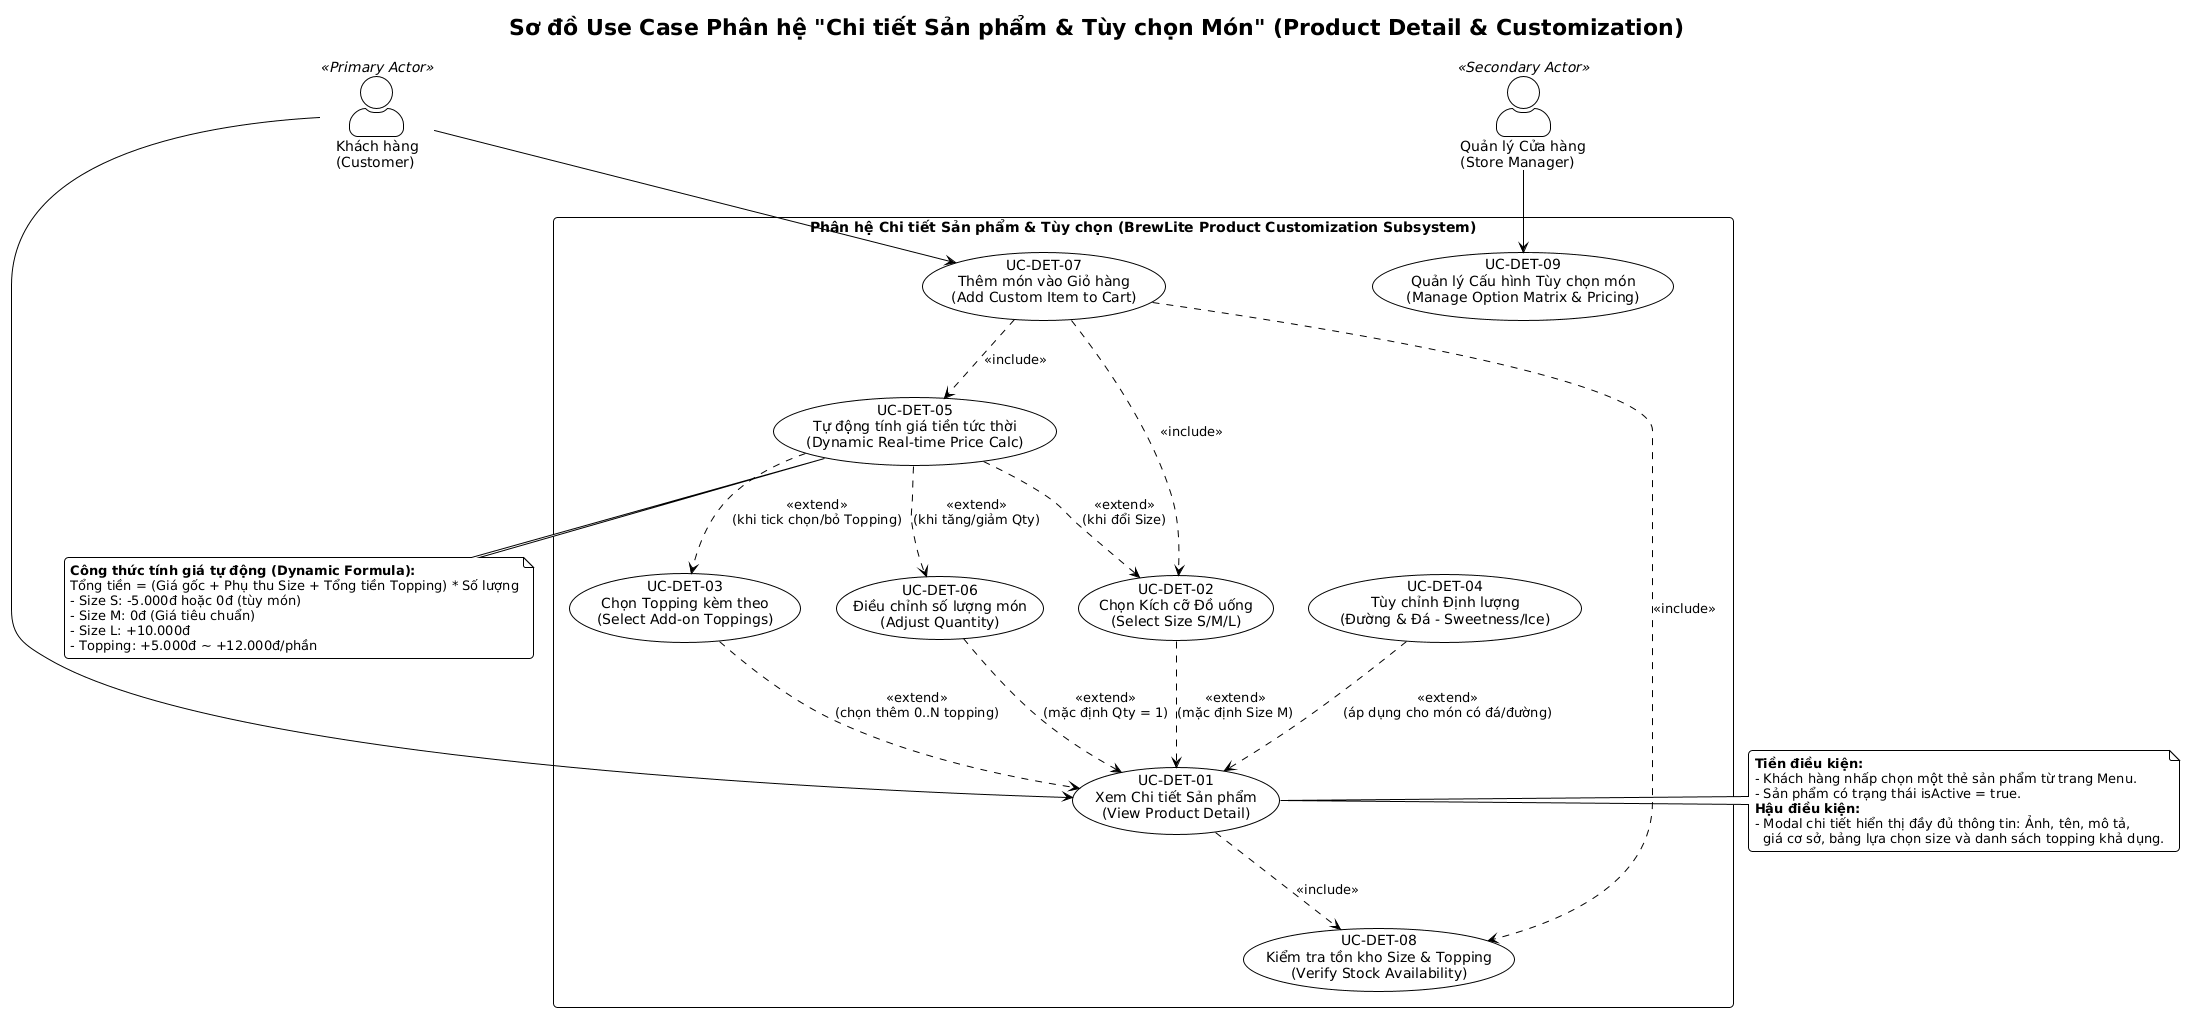
\includegraphics[width=0.88\textwidth]{usecase-detail.png}
\caption{Sơ đồ Use Case Phân hệ Chi tiết Sản phẩm \& Tùy chọn Món \\ (Mã nguồn: \texttt{docs/diagrams/usecase-detail.puml})}
\label{fig:usecase-detail}
\end{figure}

\subsubsection{Sơ đồ Hoạt động Luồng Xem Món, Chọn Size/Topping \& Tính Giá Tự Động}
\begin{figure}[H]
\centering
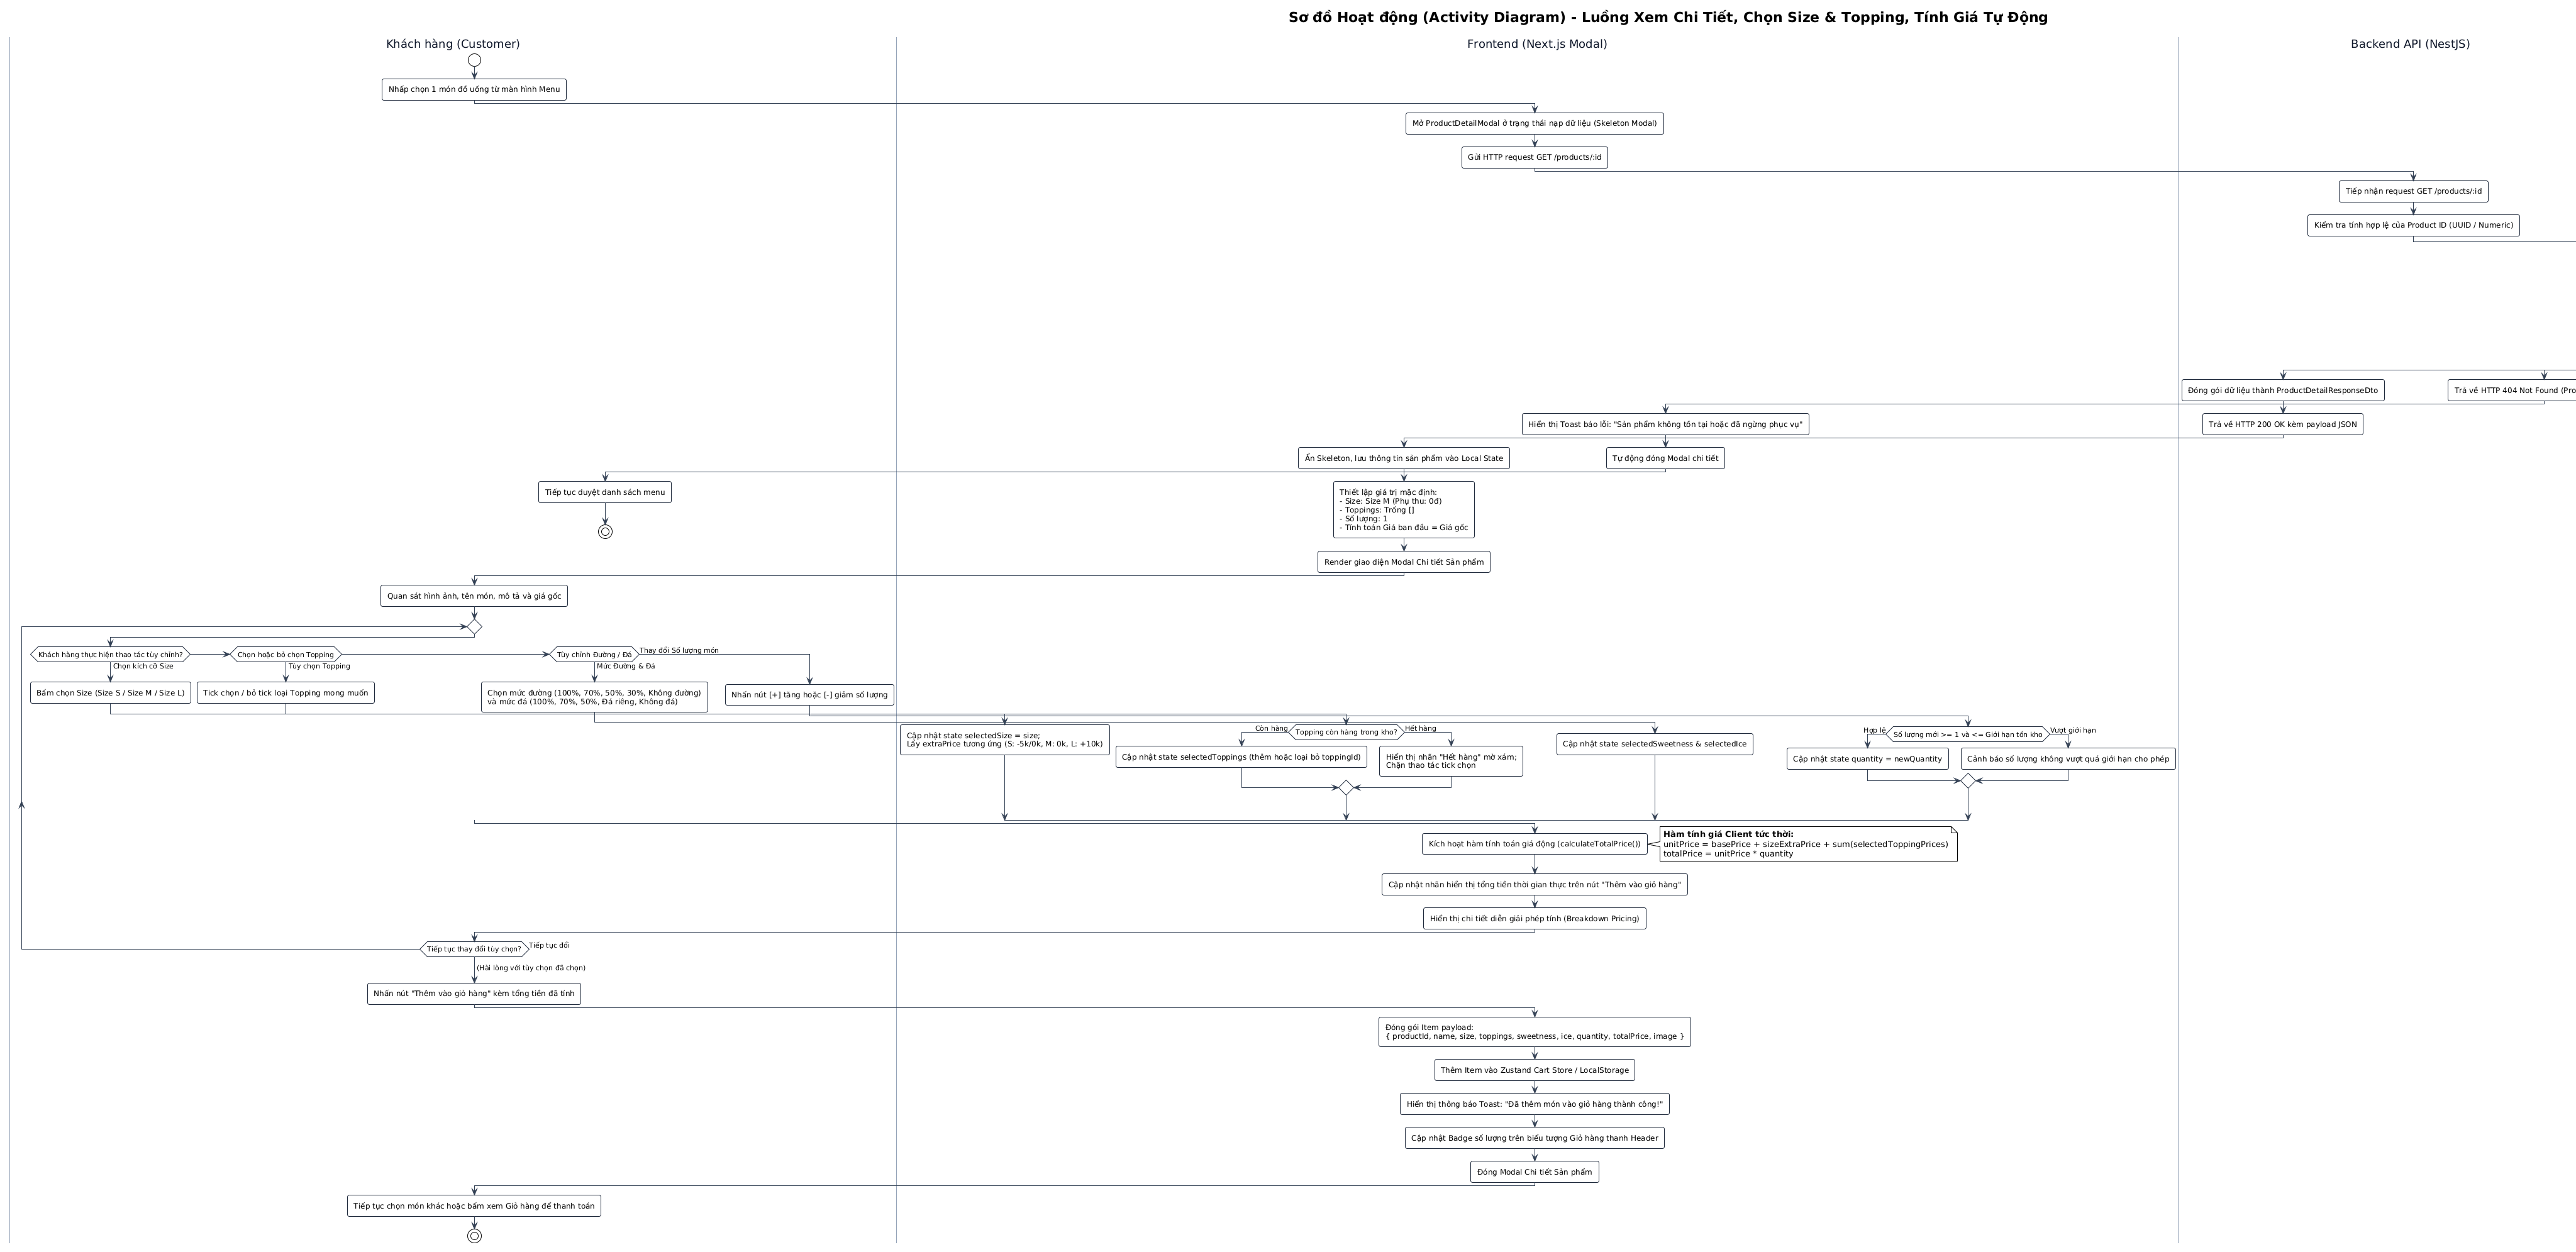
\includegraphics[width=0.88\textwidth]{activity-detail.png}
\caption{Sơ đồ Hoạt động Luồng Xem Món, Chọn Size/Topping \& Tính Giá Tự Động \\ (Mã nguồn: \texttt{docs/diagrams/activity-detail.puml})}
\label{fig:activity-detail}
\end{figure}

\subsubsection{Sơ đồ Tuần tự Gọi API Lấy Chi Tiết Sản Phẩm (\texttt{GET /products/:id})}
\begin{figure}[H]
\centering
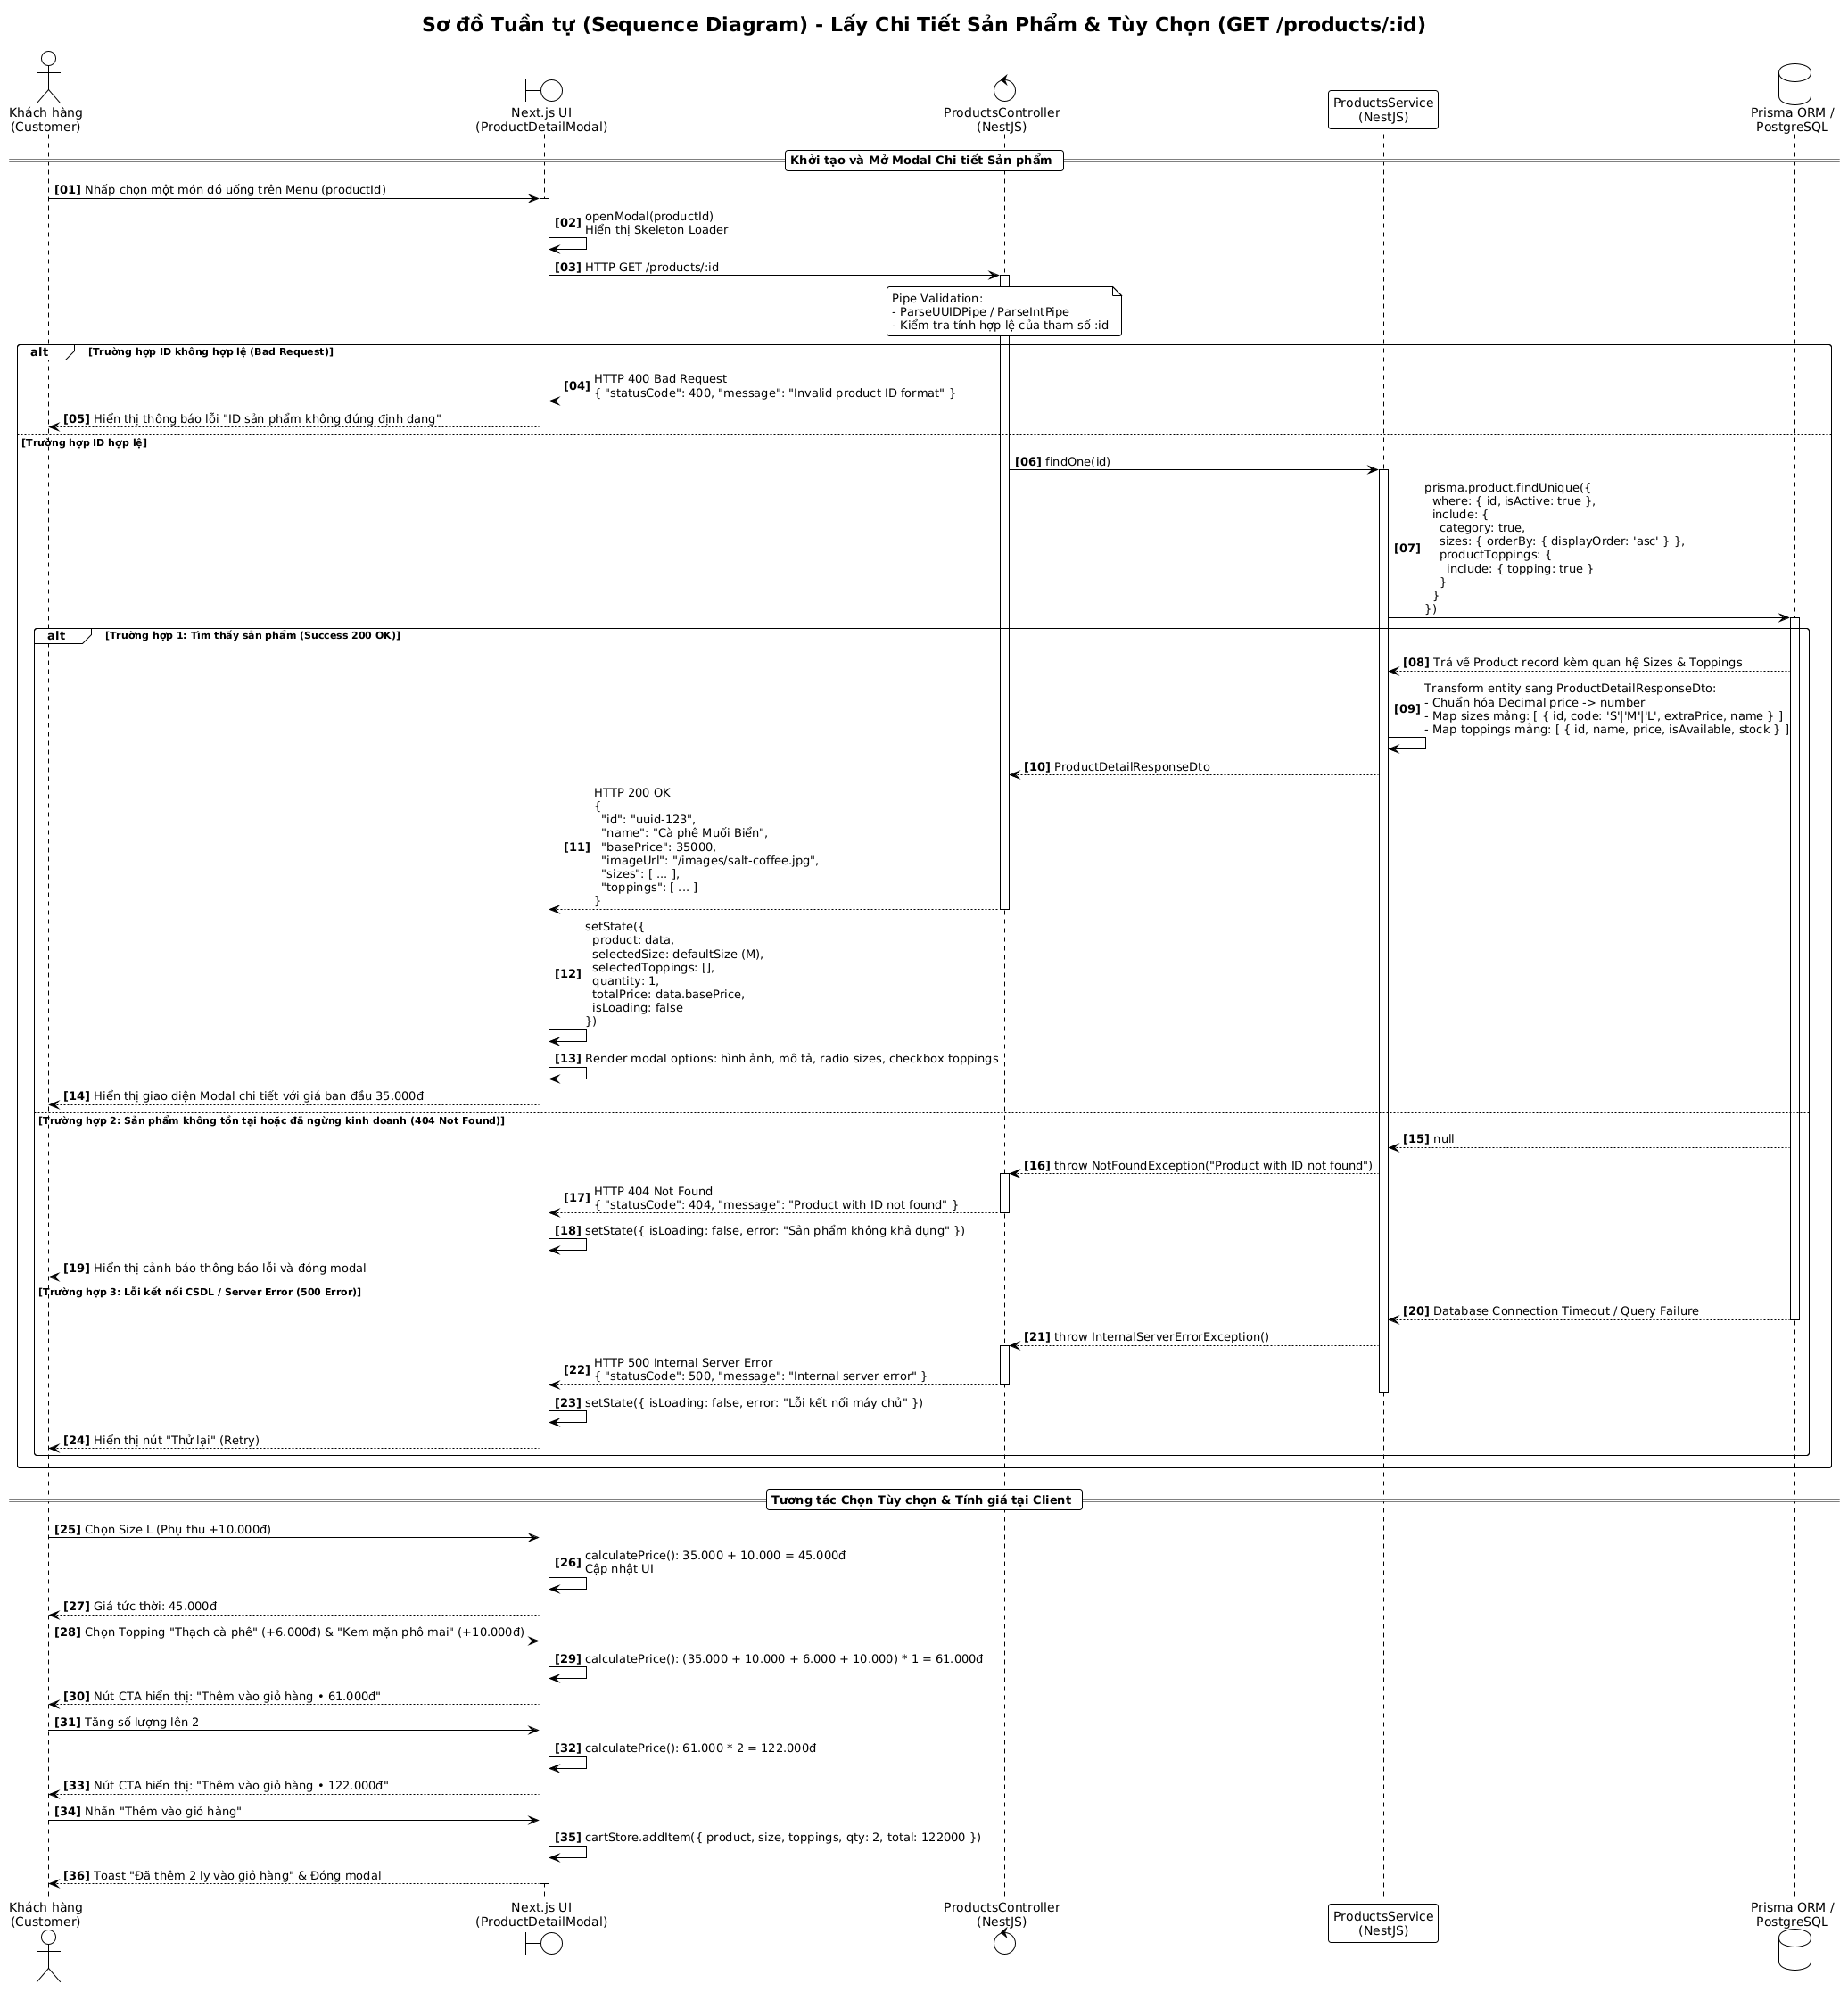
\includegraphics[width=0.88\textwidth]{sequence-detail.png}
\caption{Sơ đồ Tuần tự Gọi API Chi tiết Món và Tương tác Tính Giá \\ (Mã nguồn: \texttt{docs/diagrams/sequence-detail.puml})}
\label{fig:sequence-detail}
\end{figure}

\subsubsection{Sơ đồ Lớp Lĩnh vực ProductOption, Size \& Topping}
\begin{figure}[H]
\centering
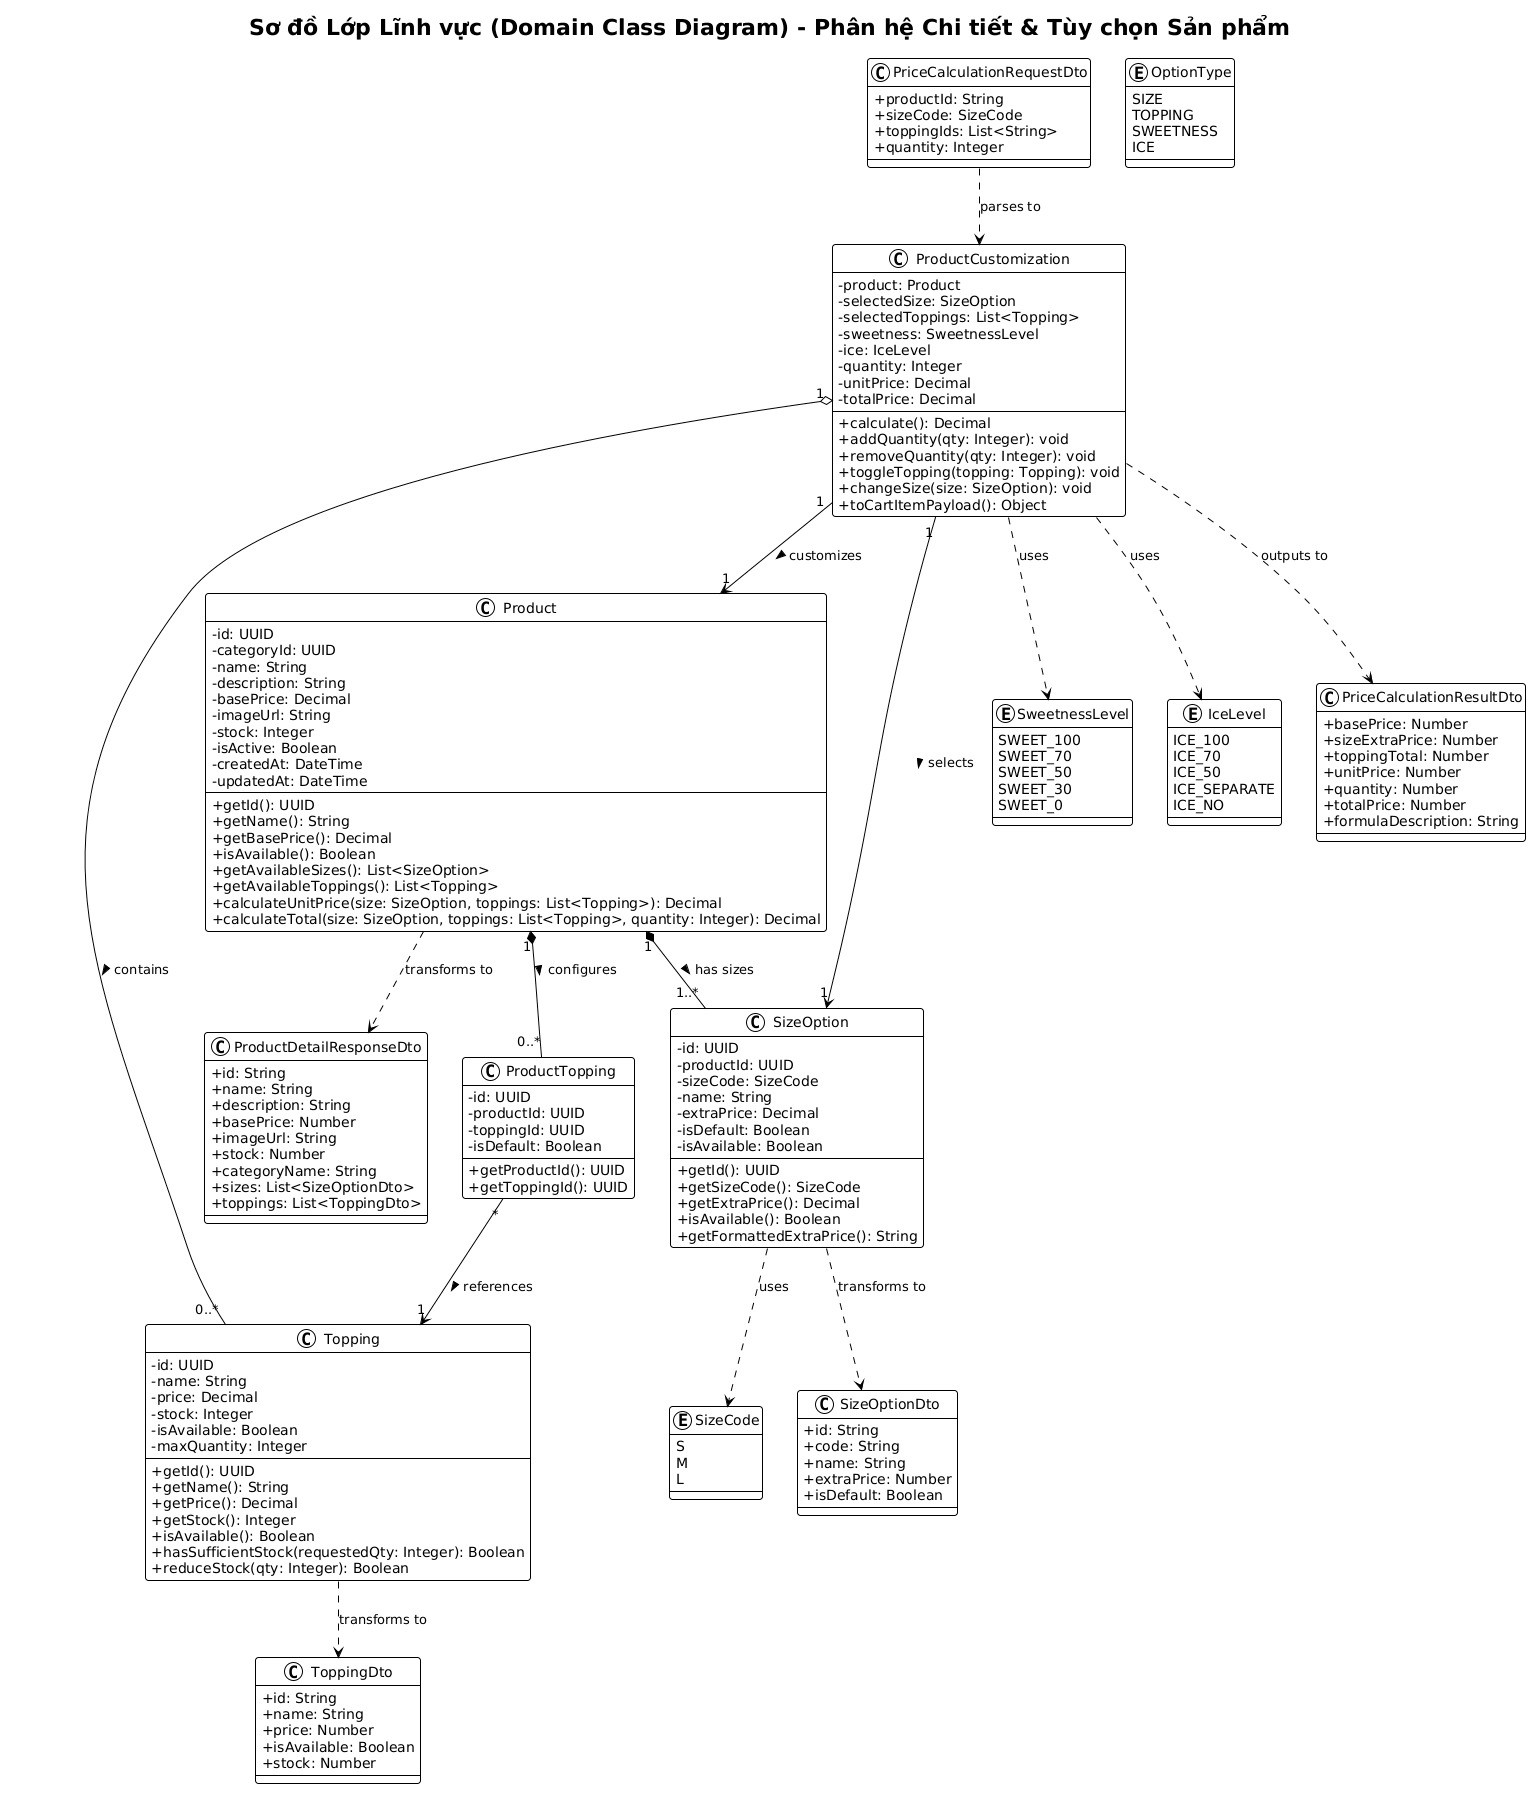
\includegraphics[width=0.88\textwidth]{class-product-option.png}
\caption{Sơ đồ Lớp Lĩnh vực ProductOption, Size \& Topping \\ (Mã nguồn: \texttt{docs/diagrams/class-product-option.puml})}
\label{fig:class-product-option}
\end{figure}

\subsubsection{Sơ đồ Triển khai Cấu trúc Lưu trữ Dữ liệu Sản phẩm trong PostgreSQL}
\begin{figure}[H]
\centering
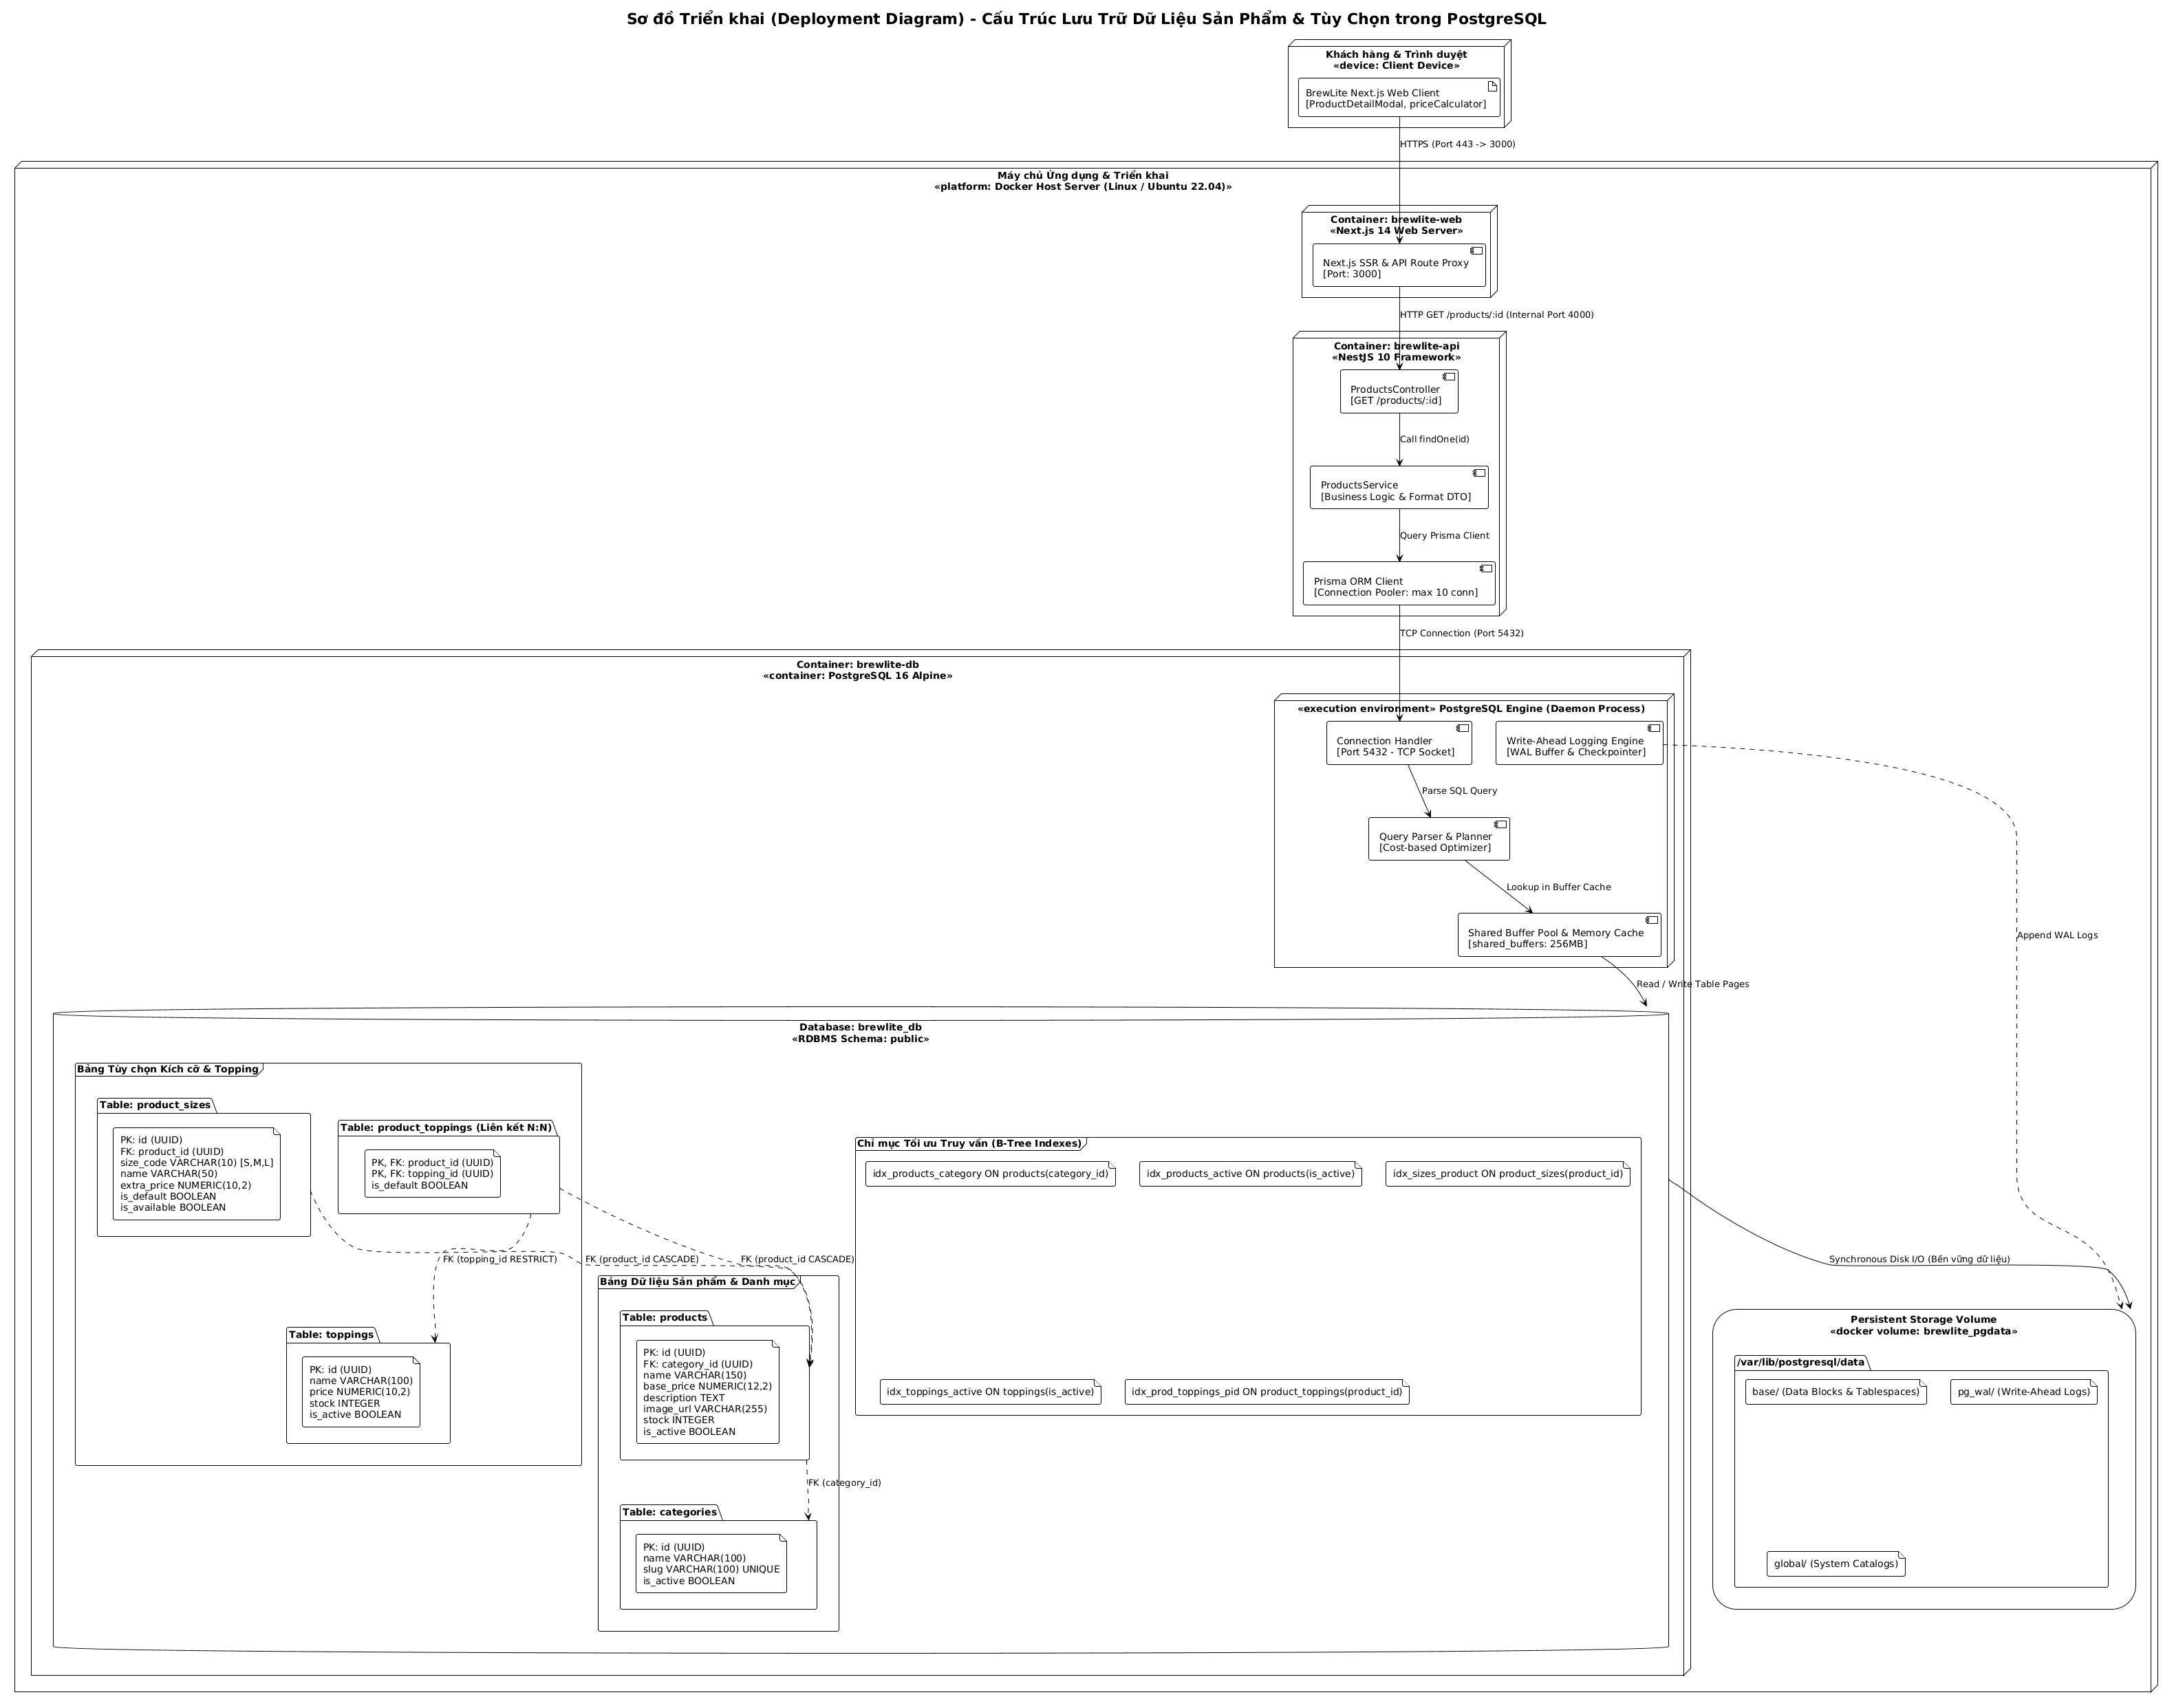
\includegraphics[width=0.88\textwidth]{deployment-product-db.png}
\caption{Sơ đồ Triển khai Cấu Trúc Lưu Trữ Dữ Liệu Sản Phẩm trong PostgreSQL \\ (Mã nguồn: \texttt{docs/diagrams/deployment-product-db.puml})}
\label{fig:deployment-product-db}
\end{figure}

\newpage
\subsection{Phân hệ 3: Giỏ hàng, Đặt đơn \& Thanh toán Idempotent (Thành viên 3 -- Phan Vũ Việt Quang)}

\subsubsection{Cụm Sơ đồ Quản lý Giỏ hàng và Khởi tạo Đơn hàng (FR-04)}

\paragraph{1. Sơ đồ Use Case Quản lý Giỏ hàng và Đặt đơn:}
\begin{figure}[H]
\centering
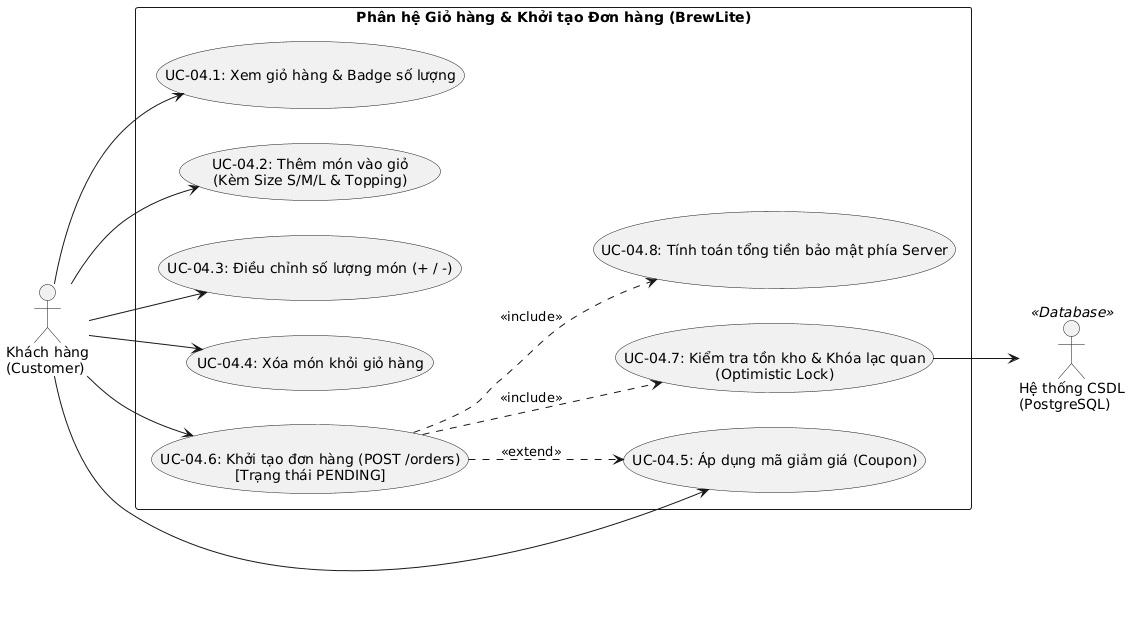
\includegraphics[width=0.86\textwidth]{usecase-cart.png}
\caption{Sơ đồ Use Case Phân hệ Quản lý Giỏ hàng và Đặt đơn hàng \\ (Mã nguồn: \texttt{docs/diagrams/usecase-cart.puml})}
\label{fig:usecase-cart}
\end{figure}

\paragraph{2. Sơ đồ Hoạt động Luồng Tương tác Giỏ hàng:}
\begin{figure}[H]
\centering
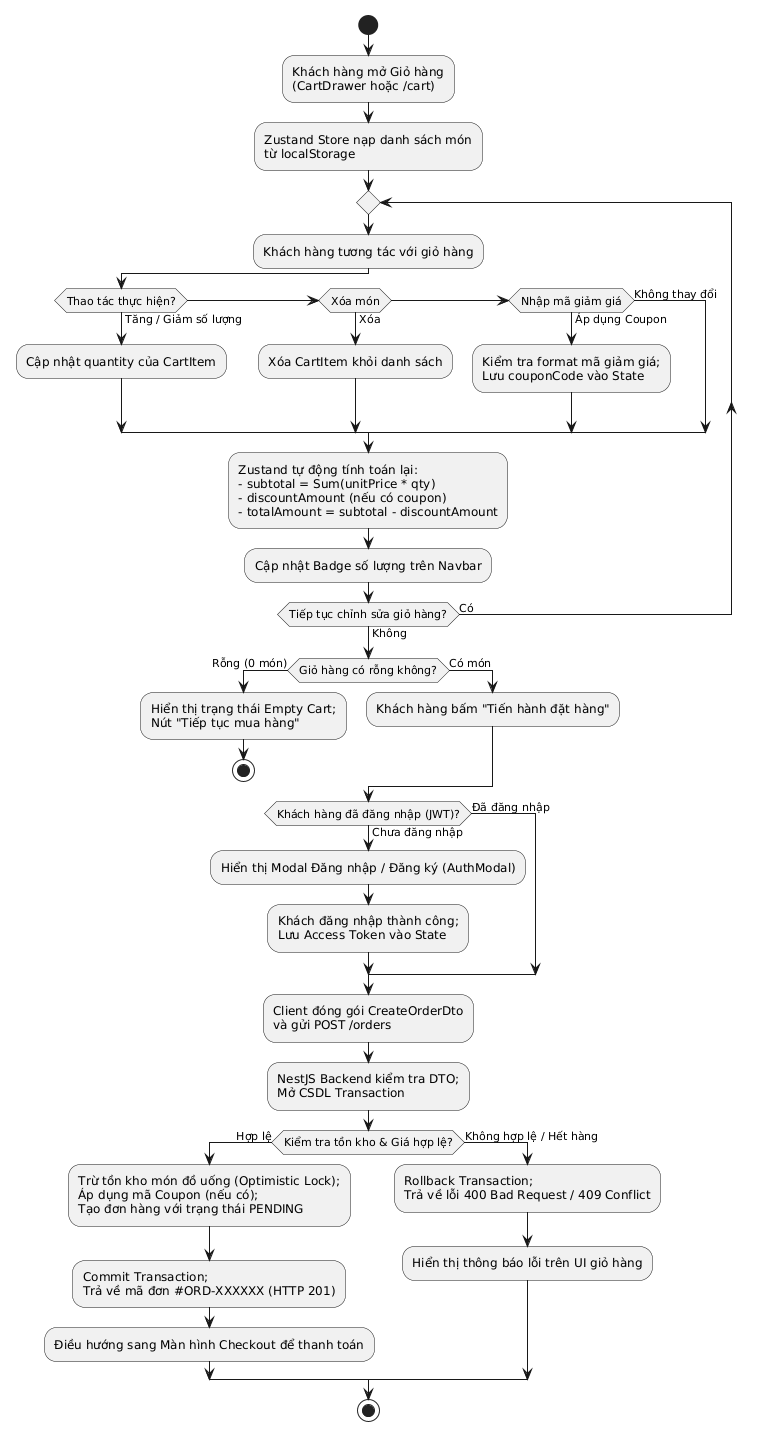
\includegraphics[width=0.86\textwidth]{activity-cart.png}
\caption{Sơ đồ Hoạt động Luồng Quản lý Giỏ hàng và Đặt đơn \\ (Mã nguồn: \texttt{docs/diagrams/activity-cart.puml})}
\label{fig:activity-cart}
\end{figure}

\paragraph{3. Sơ đồ Tuần tự Luồng Gọi API Tạo Đơn hàng (\texttt{POST /orders}):}
\begin{figure}[H]
\centering
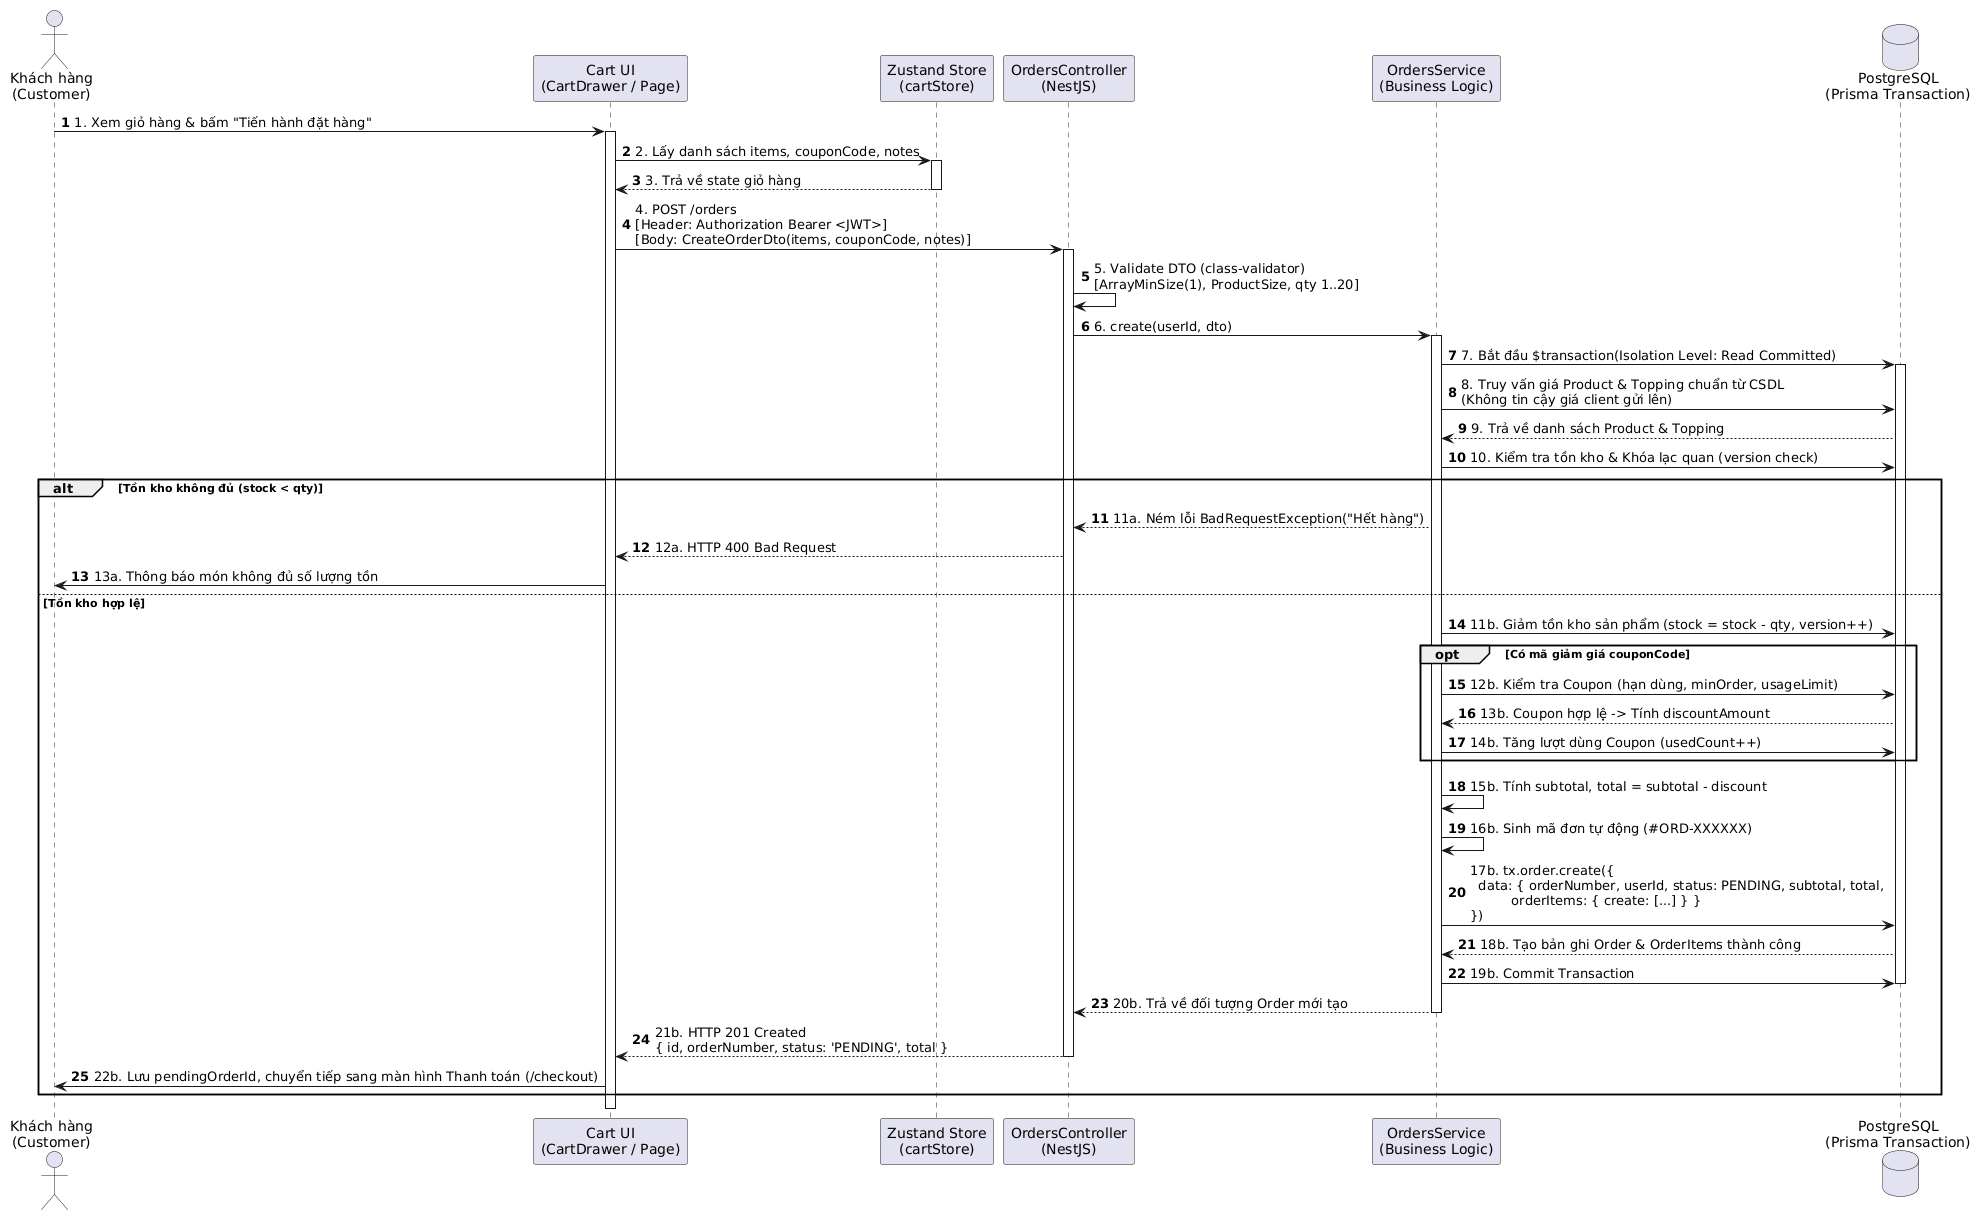
\includegraphics[width=0.86\textwidth]{sequence-order.png}
\caption{Sơ đồ Tuần tự Luồng Gọi API Tạo Đơn hàng An toàn \\ (Mã nguồn: \texttt{docs/diagrams/sequence-order.puml})}
\label{fig:sequence-order}
\end{figure}

\paragraph{4. Sơ đồ Lớp Cấu trúc Dữ liệu Giỏ hàng \& Đơn hàng:}
\begin{figure}[H]
\centering
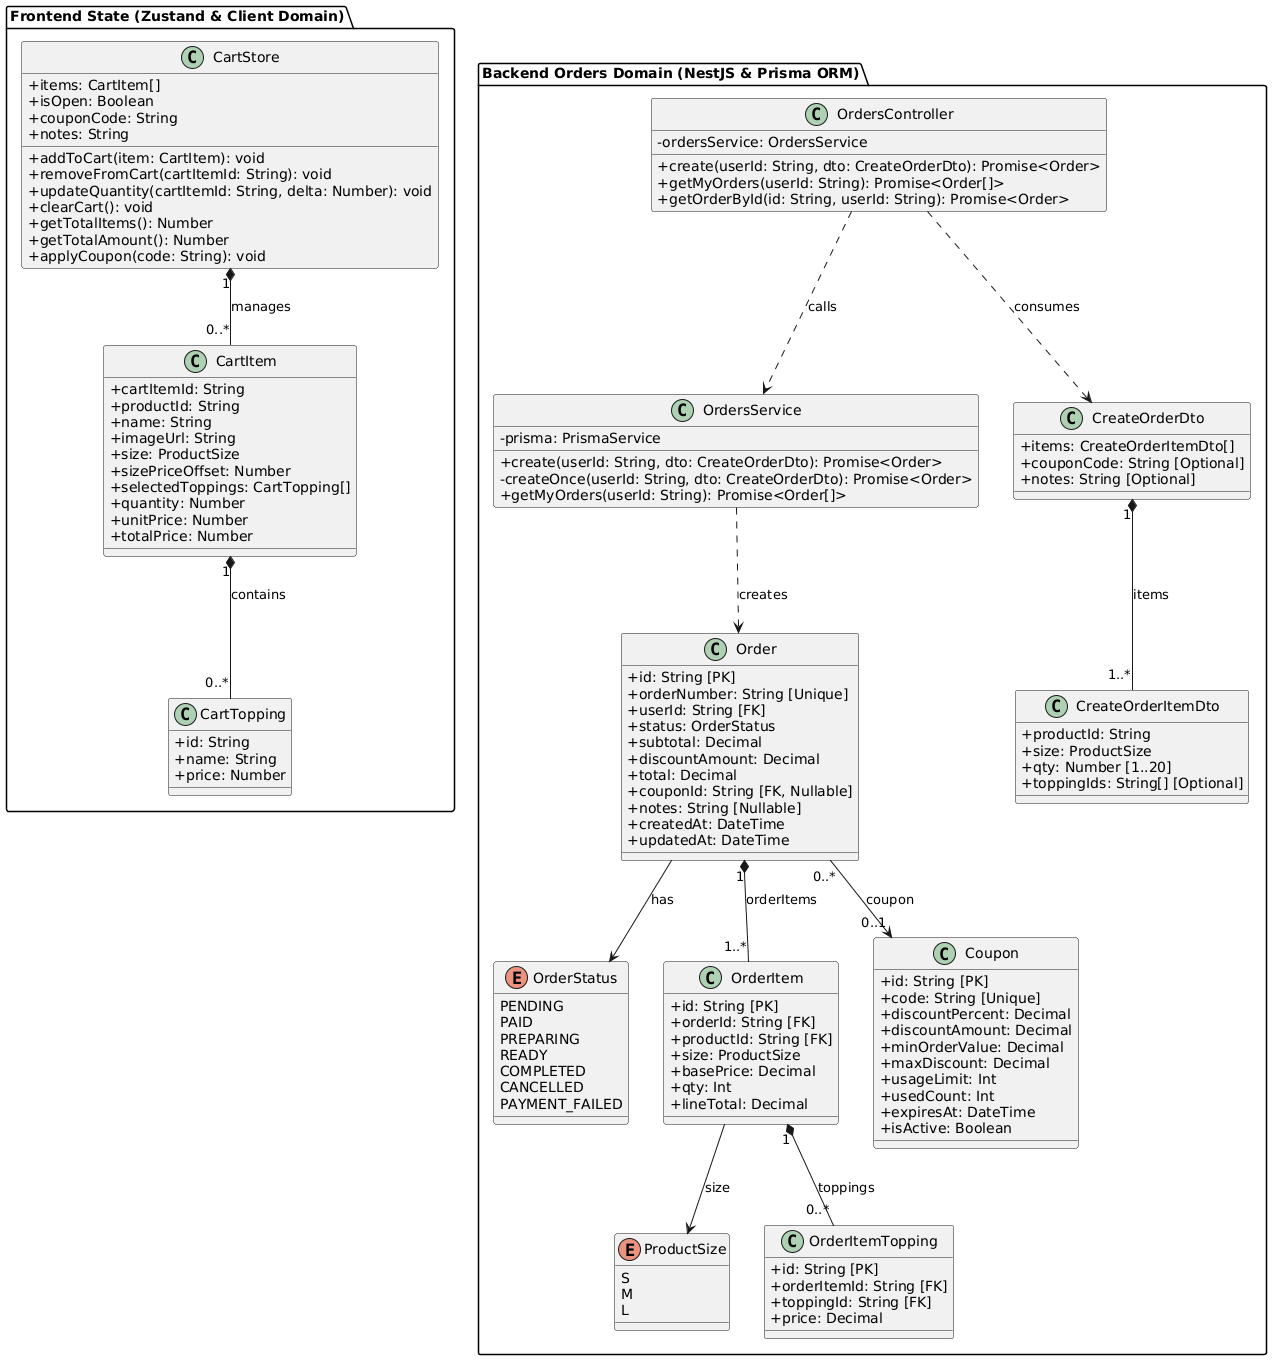
\includegraphics[width=0.86\textwidth]{class-cart-order.png}
\caption{Sơ đồ Lớp Cấu trúc Dữ liệu Giỏ hàng và Đơn hàng \\ (Mã nguồn: \texttt{docs/diagrams/class-cart-order.puml})}
\label{fig:class-cart-order}
\end{figure}

\paragraph{5. Sơ đồ Triển khai Phân hệ Giỏ hàng \& Transaction CSDL:}
\begin{figure}[H]
\centering
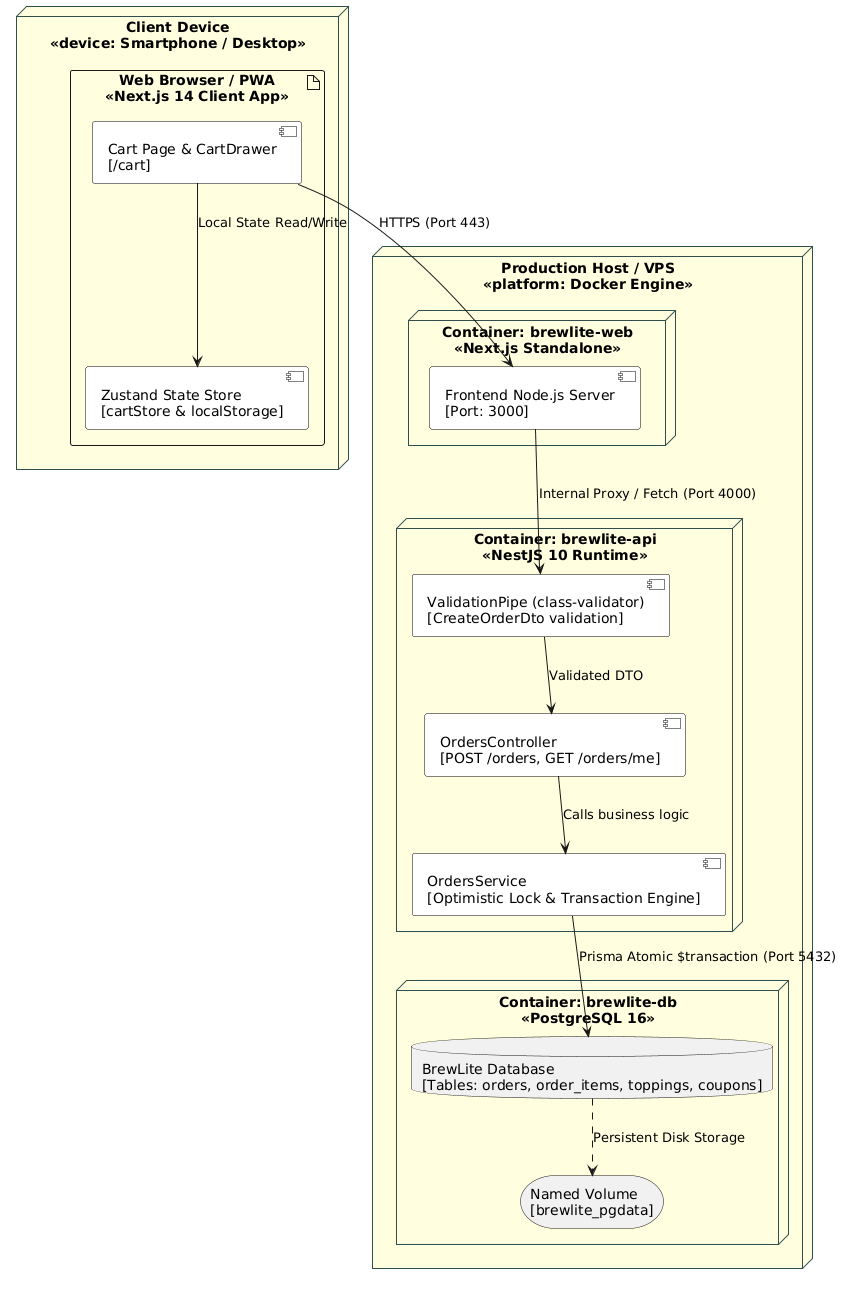
\includegraphics[width=0.86\textwidth]{deployment-cart.png}
\caption{Sơ đồ Triển khai Phân hệ Giỏ hàng và Engine Transaction CSDL \\ (Mã nguồn: \texttt{docs/diagrams/deployment-cart.puml})}
\label{fig:deployment-cart}
\end{figure}

\newpage
\subsubsection{Cụm Sơ đồ Thanh toán \& Xác nhận Đơn hàng (Task 1.3 \& FR-05/06)}

\paragraph{1. Sơ đồ Use Case Thanh toán \& Xác nhận Đơn:}
\begin{figure}[H]
\centering
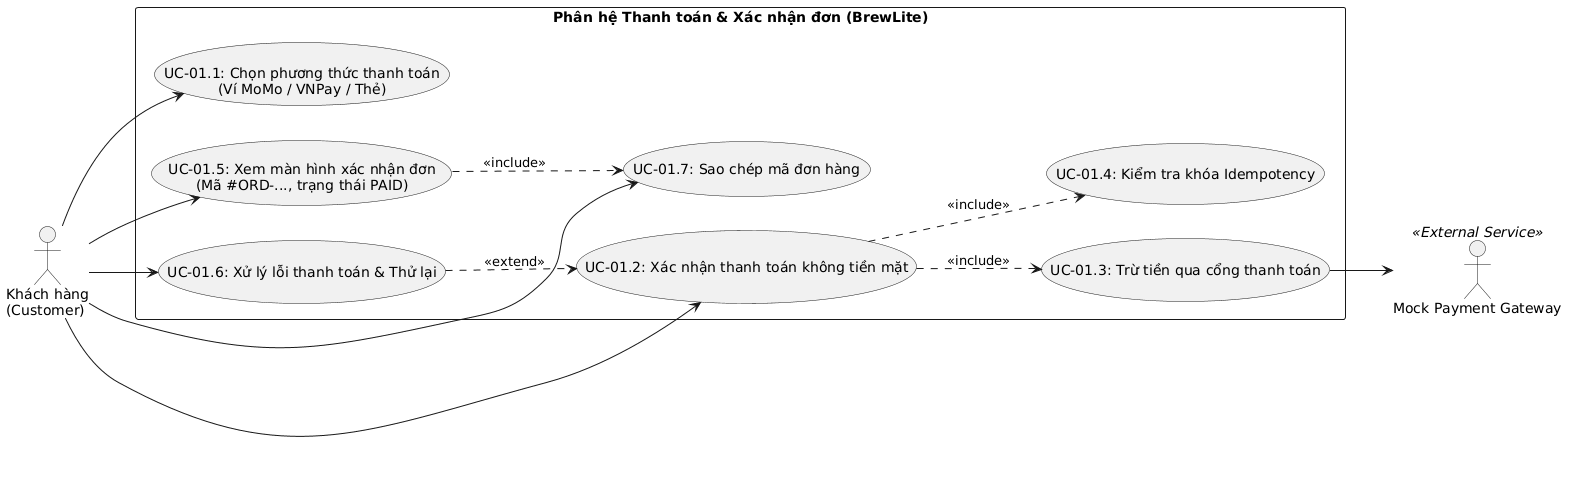
\includegraphics[width=0.86\textwidth]{usecase-payment.png}
\caption{Sơ đồ Use Case Phân hệ Thanh toán \& Xác nhận Đơn hàng \\ (Mã nguồn: \texttt{docs/diagrams/usecase-payment.puml})}
\label{fig:usecase-payment}
\end{figure}

\paragraph{2. Sơ đồ Hoạt động Luồng Thanh toán Idempotent \& Rẽ nhánh:}
\begin{figure}[H]
\centering
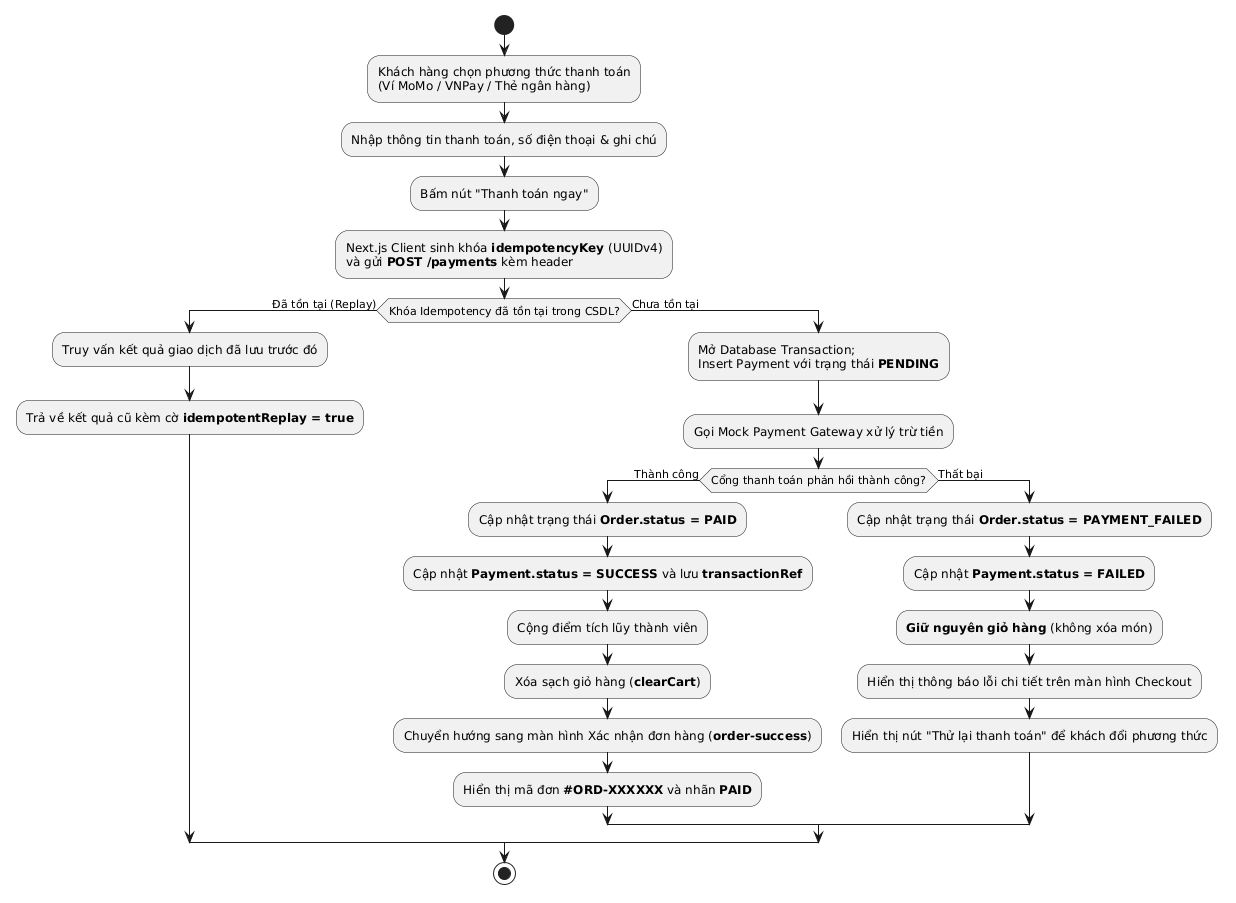
\includegraphics[width=0.86\textwidth]{activity-payment.png}
\caption{Sơ đồ Hoạt động Luồng Thanh toán Rẽ nhánh có Idempotency \\ (Mã nguồn: \texttt{docs/diagrams/activity-payment.puml})}
\label{fig:activity-payment}
\end{figure}

\paragraph{3. Sơ đồ Tuần tự Gọi API Idempotent (\texttt{POST /payments}):}
\begin{figure}[H]
\centering
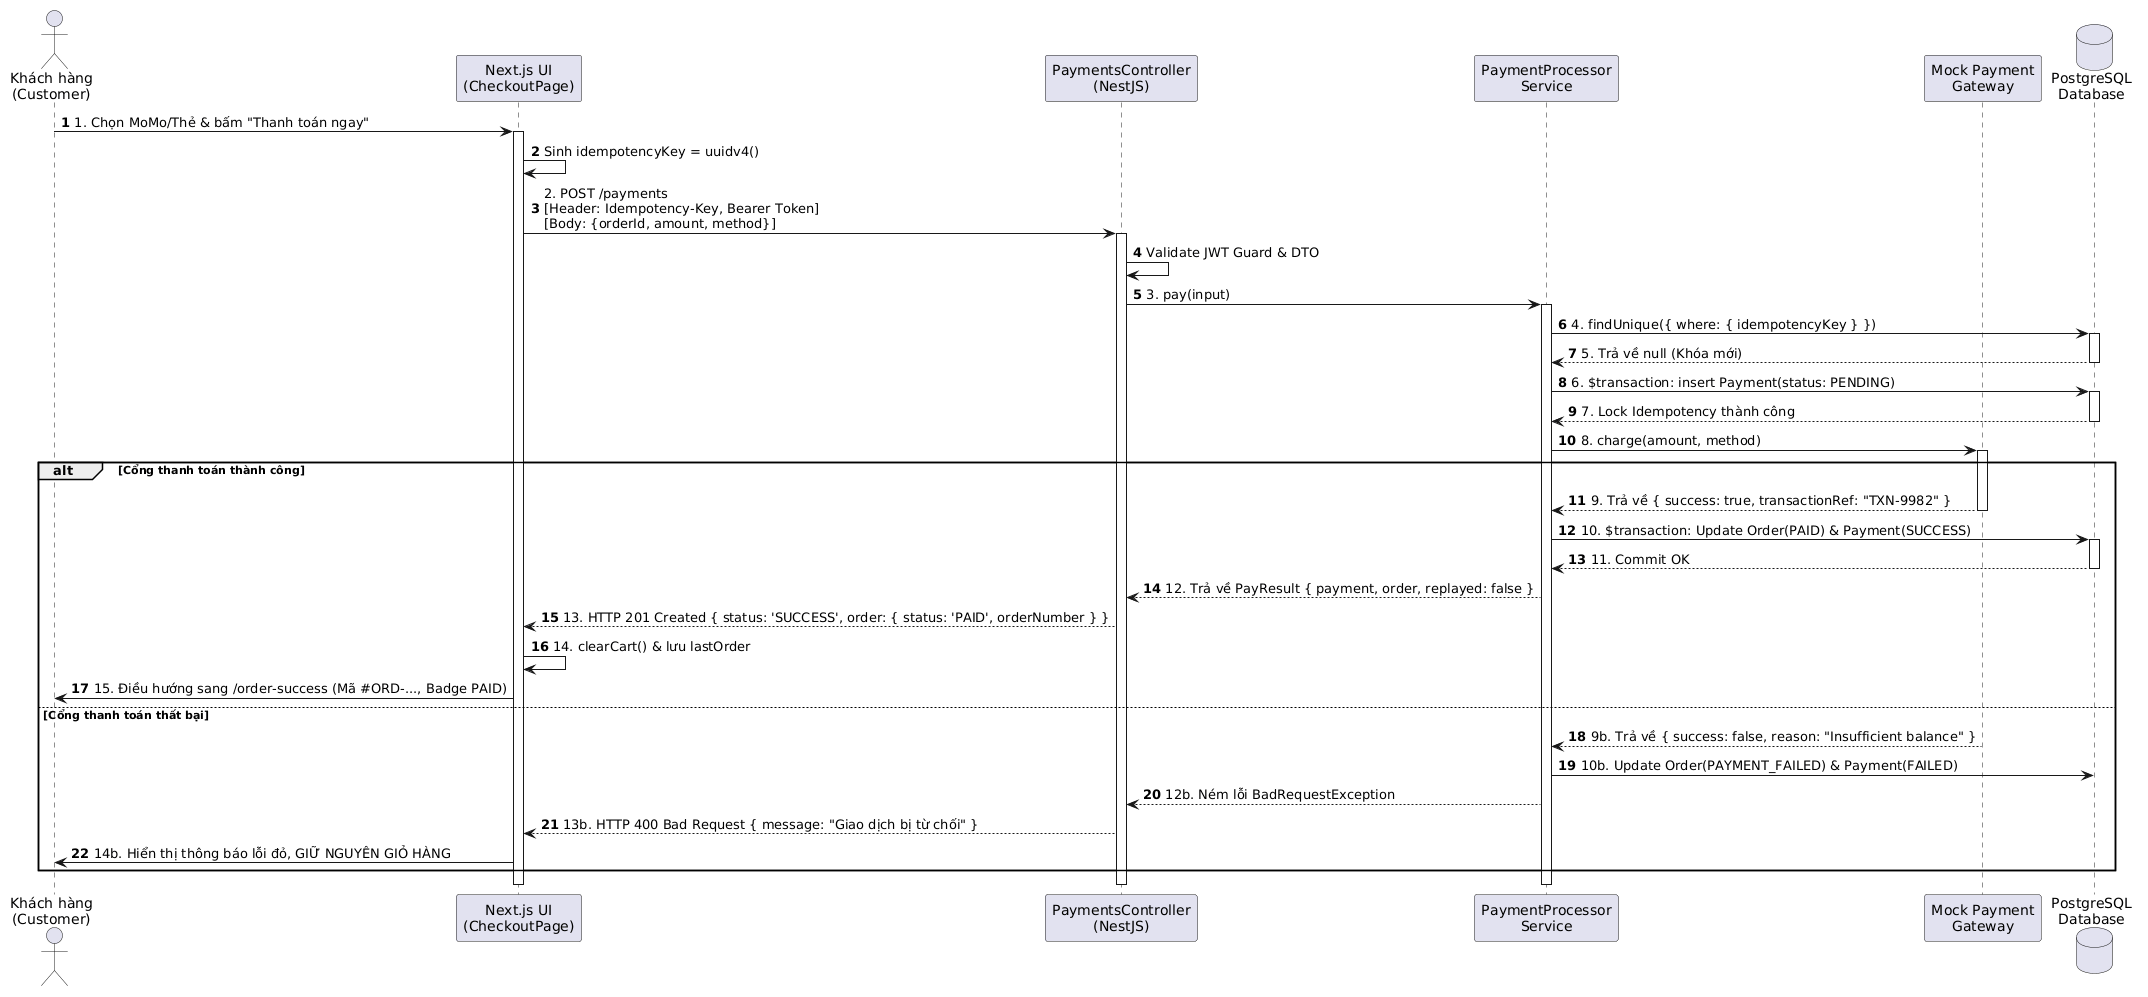
\includegraphics[width=0.86\textwidth]{sequence-payment.png}
\caption{Sơ đồ Tuần tự Gọi API Thanh toán Idempotent \\ (Mã nguồn: \texttt{docs/diagrams/sequence-payment.puml})}
\label{fig:sequence-payment}
\end{figure}

\paragraph{4. Sơ đồ Lớp Cấu trúc Dữ liệu Thanh toán \& Đơn hàng:}
\begin{figure}[H]
\centering
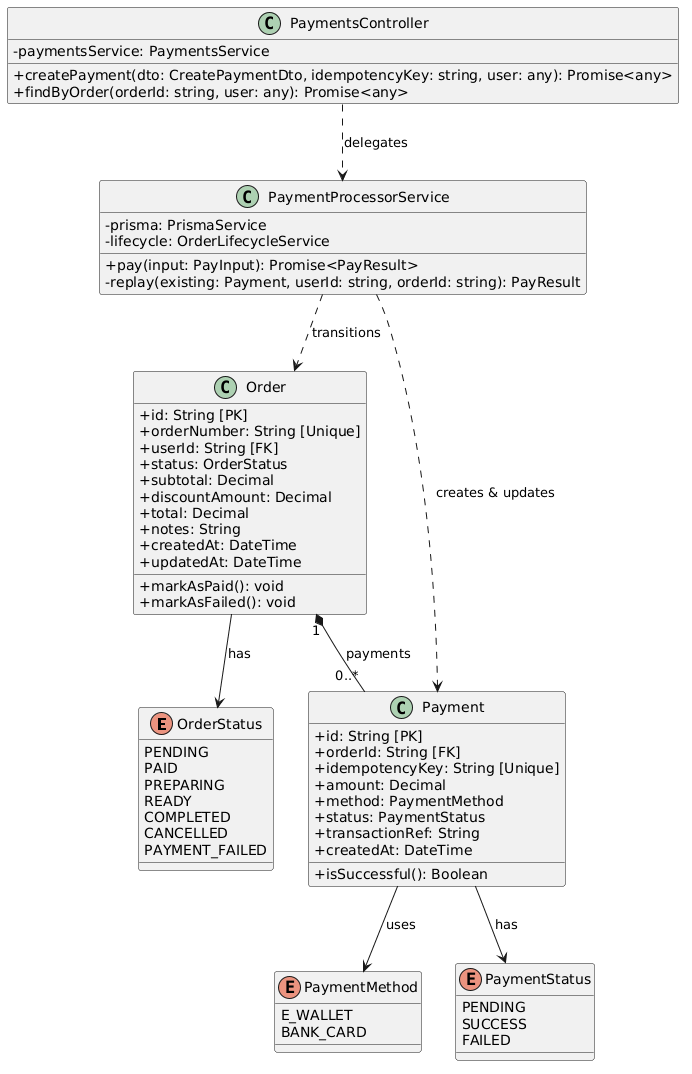
\includegraphics[width=0.86\textwidth]{class-payment.png}
\caption{Sơ đồ Lớp Cấu trúc Dữ liệu Thanh toán và Đơn hàng \\ (Mã nguồn: \texttt{docs/diagrams/class-payment.puml})}
\label{fig:class-payment}
\end{figure}

\paragraph{5. Sơ đồ Triển khai Tích hợp Nút Cổng Thanh toán Giả lập:}
\begin{figure}[H]
\centering
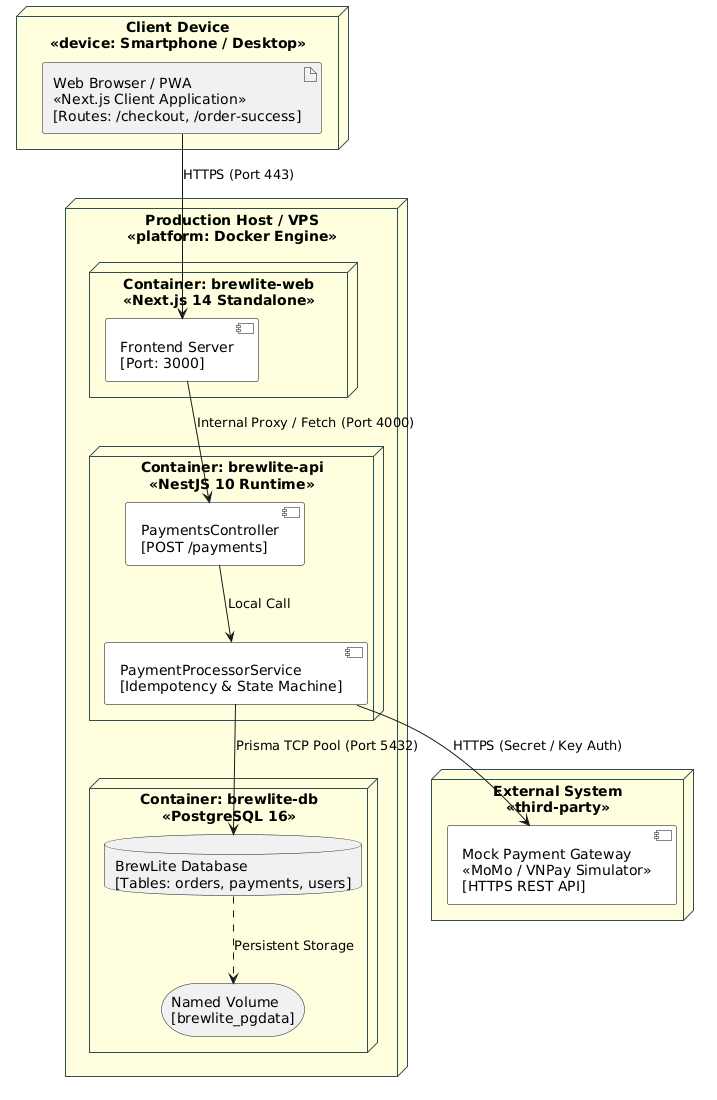
\includegraphics[width=0.86\textwidth]{deployment-payment.png}
\caption{Sơ đồ Triển khai Tích hợp Nút Cổng Thanh toán Giả lập \\ (Mã nguồn: \texttt{docs/diagrams/deployment-payment.puml})}
\label{fig:deployment-payment}
\end{figure}

\newpage
\subsection{Phân hệ 4: Đăng nhập, Đăng ký \& Bảo mật Hạ tầng Docker (Thành viên 4 -- Nguyễn Hữu Chí Công)}

\subsubsection{Sơ đồ Use Case Phân hệ Xác thực \& Phân quyền JWT}
\begin{figure}[H]
\centering
\resizebox{0.94\linewidth}{!}{
\begin{tikzpicture}[
    actor/.style={circle, draw=black!85, fill=blue!8, thick, minimum size=0.95cm, font=\bfseries\scriptsize, align=center},
    uc/.style={ellipse, draw=black!85, fill=white, thick, minimum height=0.82cm, minimum width=3.6cm, align=center, font=\scriptsize\bfseries},
    subuc/.style={ellipse, draw=black!75, fill=gray!8, thick, minimum height=0.78cm, minimum width=3.5cm, align=center, font=\scriptsize},
    arrow/.style={thick, draw=black!85},
    darrow/.style={thick, dashed, ->, >=stealth, draw=black!75}
]
    % Actors
    \node[actor] (guest) at (-1.5, 2.6) {Khách vãng lai\\(Guest)};
    \node[actor, fill=green!10] (member) at (-1.5, -2.0) {Người dùng\\Đã xác thực};

    % System Boundary
    \draw[thick, dashed, gray!70, rounded corners=6pt] (1.0, -4.5) rectangle (12.6, 4.8);
    \node[font=\small\bfseries, text=black!90, anchor=north west] at (1.2, 4.6) {Phân hệ Xác thực \& Phân quyền JWT (BrewLite Auth Subsystem)};

    % Primary Use Cases
    \node[uc] (uc1) at (3.8, 3.2) {UC-AUTH-01: Đăng ký tài khoản\\(\texttt{POST /auth/register})};
    \node[uc] (uc4) at (3.8, 1.2) {UC-AUTH-04: Đăng nhập hệ thống\\(\texttt{POST /auth/login})};
    \node[uc] (uc7) at (3.8, -0.8) {UC-AUTH-07: Xem hồ sơ \& Điểm\\(\texttt{GET /auth/me})};
    \node[uc] (uc8) at (3.8, -2.3) {UC-AUTH-08: Bảo vệ Route Đặt đơn\\(\texttt{JwtAuthGuard \& RolesGuard})};
    \node[uc] (uc9) at (3.8, -3.7) {UC-AUTH-09: Đăng xuất tài khoản\\(Xóa LocalStorage Token)};

    % Included Sub Use Cases
    \node[subuc] (uc2) at (9.8, 3.8) {UC-AUTH-02: Kiểm tra SĐT 10 số\\\& Email \texttt{@unique}};
    \node[subuc] (uc3) at (9.8, 2.2) {UC-AUTH-03: Băm mật khẩu Bcrypt\\(\texttt{Salt Rounds = 10})};
    \node[subuc] (uc5) at (9.8, 0.6) {UC-AUTH-05: Đối chiếu mật khẩu\\(\texttt{bcrypt.compare})};
    \node[subuc, fill=yellow!12] (uc6) at (9.8, -1.2) {UC-AUTH-06: Ký \& Cấp phát JWT\\(\texttt{HS256, expiresIn: 7d})};

    % Actor links
    \draw[arrow] (guest) -- (uc1);
    \draw[arrow] (guest) -- (uc4);
    \draw[arrow] (member) -- (uc7);
    \draw[arrow] (member) -- (uc8);
    \draw[arrow] (member) -- (uc9);

    % Include / Extend links
    \draw[darrow] (uc1) -- node[above, sloped, font=\tiny] {\textless\textless include\textgreater\textgreater} (uc2);
    \draw[darrow] (uc1) -- node[above, sloped, font=\tiny] {\textless\textless include\textgreater\textgreater} (uc3);
    \draw[darrow] (uc1) -- node[above, sloped, font=\tiny, pos=0.65] {\textless\textless include\textgreater\textgreater} (uc6);
    \draw[darrow] (uc4) -- node[above, sloped, font=\tiny] {\textless\textless include\textgreater\textgreater} (uc5);
    \draw[darrow] (uc4) -- node[below, sloped, font=\tiny] {\textless\textless include\textgreater\textgreater} (uc6);
    \draw[darrow] (uc8) -- node[right, font=\tiny] {\textless\textless extend\textgreater\textgreater} (uc4);
\end{tikzpicture}
}
\caption{Sơ đồ Use Case Phân hệ Đăng nhập, Đăng ký \& Quản lý Tài khoản (Mã nguồn: \nolinkurl{docs/diagrams/usecase-auth.puml})}
\label{fig:usecase_auth}
\end{figure}

\subsubsection{Sơ đồ Hoạt động Luồng Đăng ký, Đăng nhập \& Xác thực Bcrypt}
\begin{figure}[H]
\centering
\resizebox{0.95\linewidth}{!}{
\begin{tikzpicture}[
    node distance=0.8cm,
    act/.style={rectangle, rounded corners=4pt, draw=black!85, fill=white, thick, text width=3.3cm, minimum height=0.75cm, align=center, font=\scriptsize},
    dec/.style={diamond, aspect=2.1, draw=black!85, fill=yellow!10, thick, inner sep=1.5pt, align=center, font=\scriptsize\bfseries},
    err/.style={rectangle, rounded corners=4pt, draw=red!80!black, fill=red!8, thick, text width=3.1cm, minimum height=0.65cm, align=center, font=\scriptsize},
    arrow/.style={thick, ->, >=stealth, draw=black!85}
]
    % Swimlane headers
    \draw[thick, fill=gray!12] (0, 8.2) rectangle (15.6, 8.9);
    \draw[thick] (0, -4.6) rectangle (15.6, 8.9);
    \draw[dashed, gray!70] (3.9, -4.6) -- (3.9, 8.9);
    \draw[dashed, gray!70] (7.8, -4.6) -- (7.8, 8.9);
    \draw[dashed, gray!70] (11.7, -4.6) -- (11.7, 8.9);

    \node[font=\scriptsize\bfseries] at (1.95, 8.55) {Người dùng (User)};
    \node[font=\scriptsize\bfseries] at (5.85, 8.55) {Frontend (Next.js AuthModal)};
    \node[font=\scriptsize\bfseries] at (9.75, 8.55) {Backend (NestJS AuthService)};
    \node[font=\scriptsize\bfseries] at (13.65, 8.55) {Database (PostgreSQL)};

    % Nodes
    \node[circle, fill=black, minimum size=0.35cm] (start) at (1.95, 7.6) {};
    \node[act] (open) at (1.95, 6.5) {Mở AuthModal trên Navbar \& chọn Tab Đăng ký / Đăng nhập};
    \node[dec] (mode) at (5.85, 6.5) {Chế độ nào?};

    % Register path
    \node[act] (inputReg) at (1.95, 4.7) {Nhập Họ tên, SĐT (10 số), Email, Mật khẩu ($\ge 6$ ký tự)};
    \node[dec] (valPhone) at (5.85, 4.7) {SĐT đủ 10 số?};
    \node[err] (errPhone) at (5.85, 3.2) {Báo lỗi định dạng SĐT ngay dưới ô nhập};
    \node[act] (postReg) at (9.75, 4.7) {\texttt{POST /auth/register}\\Chuẩn hóa email};
    \node[dec] (dupEmail) at (13.65, 4.7) {Trùng Email?};
    \node[err] (err409) at (9.75, 3.2) {Trả lỗi \texttt{409 Conflict}\\(Email đã tồn tại)};
    \node[act, fill=green!8] (hashPwd) at (9.75, 1.8) {Băm mật khẩu Bcrypt:\\\texttt{bcrypt.hash(pwd, 10)}};
    \node[act] (insertUser) at (13.65, 1.8) {\texttt{INSERT INTO users}\\(role=CUSTOMER, points=0)};

    % Login path
    \node[act] (inputLogin) at (1.95, 0.3) {Nhập Email \& Mật khẩu\\Bấm ``Đăng nhập''};
    \node[act] (postLogin) at (5.85, 0.3) {Gửi \texttt{POST /auth/login}};
    \node[dec] (cmpHash) at (9.75, 0.3) {\texttt{bcrypt.compare()}\\khớp mật khẩu?};
    \node[err] (err401) at (9.75, -1.2) {Trả lỗi \texttt{401 Unauthorized}\\(Sai email / mật khẩu)};

    % Merge & JWT Sign
    \node[act, fill=blue!8] (signJwt) at (9.75, -2.6) {Ký \texttt{JWT Access Token} (HS256, 7d) \& ẩn \texttt{passwordHash}};
    \node[act, fill=green!8] (saveStore) at (5.85, -2.6) {Lưu \texttt{setAuth(user, token)} vào Zustand \texttt{localStorage}};
    \node[act] (finish) at (1.95, -2.6) {Cập nhật Navbar, mở khóa Đặt đơn (hoặc chuyển \texttt{/orders} nếu Barista)};
    \node[circle, draw=black, thick, minimum size=0.45cm] (stopOuter) at (1.95, -4.0) {};
    \node[circle, fill=black, minimum size=0.25cm] (stopInner) at (1.95, -4.0) {};

    % Edges
    \draw[arrow] (start) -- (open);
    \draw[arrow] (open) -- (mode);
    \draw[arrow] (mode) -- node[above, font=\tiny] {Đăng ký} (inputReg);
    \draw[arrow] (inputReg) -- (valPhone);
    \draw[arrow] (valPhone) -- node[right, font=\tiny] {Sai} (errPhone);
    \draw[arrow] (valPhone) -- node[above, font=\tiny] {Hợp lệ} (postReg);
    \draw[arrow] (postReg) -- (dupEmail);
    \draw[arrow] (dupEmail) |- node[above, pos=0.7, font=\tiny] {Có} (err409);
    \draw[arrow] (dupEmail) -- node[right, font=\tiny] {Chưa có} (insertUser);
    \draw[arrow] (insertUser) -- (hashPwd);

    \draw[arrow] (mode.south) -- ++(0,-0.4) -| node[pos=0.25, above, font=\tiny] {Đăng nhập} (inputLogin.north);
    \draw[arrow] (inputLogin) -- (postLogin);
    \draw[arrow] (postLogin) -- (cmpHash);
    \draw[arrow] (cmpHash) -- node[right, font=\tiny] {Sai} (err401);

    \draw[arrow] (hashPwd.west) -- ++(-0.5,0) |- (signJwt.west);
    \draw[arrow] (cmpHash.east) -- ++(0.6,0) |- node[pos=0.2, right, font=\tiny] {Đúng} (signJwt.east);
    \draw[arrow] (signJwt) -- (saveStore);
    \draw[arrow] (saveStore) -- (finish);
    \draw[arrow] (finish) -- (stopOuter);
\end{tikzpicture}
}
\caption{Sơ đồ Hoạt động Luồng Đăng ký, Đăng nhập, Xác thực Bcrypt và Lưu JWT Token (Mã nguồn: \nolinkurl{docs/diagrams/activity-auth.puml})}
\label{fig:activity_auth}
\end{figure}

\subsubsection{Sơ đồ Tuần tự API Đăng ký, Đăng nhập \& JwtAuthGuard}
\begin{figure}[H]
\centering
\resizebox{0.96\linewidth}{!}{
\begin{tikzpicture}[
    lifeline/.style={rectangle, draw=black!85, fill=gray!10, thick, minimum width=2.4cm, minimum height=0.8cm, align=center, font=\scriptsize\bfseries},
    msg/.style={->, >=stealth, thick, draw=black!85},
    ret/.style={->, >=stealth, thick, dashed, draw=black!70}
]
    % Participants
    \node[lifeline] (p1) at (0, 0) {Người dùng\\(User)};
    \node[lifeline] (p2) at (3.4, 0) {Next.js UI\\(AuthModal)};
    \node[lifeline] (p3) at (6.8, 0) {AuthController\\\& JwtAuthGuard};
    \node[lifeline] (p4) at (10.2, 0) {AuthService\\\& JwtService};
    \node[lifeline, fill=green!10] (p5) at (13.6, 0) {PostgreSQL\\(Prisma ORM)};

    % Vertical dashed lines
    \foreach \p in {p1,p2,p3,p4,p5} {
        \draw[dashed, gray!70, thick] (\p.south) -- ++(0, -10.6);
    }

    % Flow 1: Register
    \draw[fill=blue!6, draw=blue!40] (-1.0, -1.0) rectangle (14.6, -1.5);
    \node[font=\scriptsize\bfseries] at (6.8, -1.25) {Luồng 1: Đăng ký Tài khoản Mới (\texttt{POST /auth/register})};

    \draw[msg] (0, -2.0) -- node[above, font=\tiny] {1. Nhập Họ tên, SĐT (10 số), Email, Mật khẩu} (3.4, -2.0);
    \draw[msg] (3.4, -2.6) -- node[above, font=\tiny] {2. \texttt{POST /auth/register \{email, password, fullName, phone\}}} (6.8, -2.6);
    \draw[msg] (6.8, -3.2) -- node[above, font=\tiny] {3. \texttt{register(dto)} (ValidationPipe)} (10.2, -3.2);
    \draw[msg] (10.2, -3.8) -- node[above, font=\tiny] {4. \texttt{user.findUnique(\{ email \})}} (13.6, -3.8);
    \draw[ret] (13.6, -4.3) -- node[above, font=\tiny] {5. \texttt{null} (Email hợp lệ)} (10.2, -4.3);
    \draw[msg] (10.2, -4.9) -- node[above, font=\tiny] {6. \texttt{bcrypt.hash(pwd, 10)} $\rightarrow$ \texttt{user.create()}} (13.6, -4.9);
    \draw[ret] (13.6, -5.4) -- node[above, font=\tiny] {7. Bản ghi \texttt{User(role=CUSTOMER)}} (10.2, -5.4);
    \draw[ret] (10.2, -6.0) -- node[above, font=\tiny] {8. \texttt{jwtService.signAsync()} $\rightarrow$ \texttt{HTTP 201 \{access\_token, user\}}} (3.4, -6.0);
    \draw[ret] (3.4, -6.5) -- node[above, font=\tiny] {9. \texttt{setAuth(user, token)} \& Đóng Modal} (0, -6.5);

    % Flow 2: Login
    \draw[fill=blue!6, draw=blue!40] (-1.0, -7.1) rectangle (14.6, -7.6);
    \node[font=\scriptsize\bfseries] at (6.8, -7.35) {Luồng 2: Đăng nhập (\texttt{POST /auth/login}) \& Bảo vệ Route (\texttt{JwtAuthGuard})};

    \draw[msg] (0, -8.1) -- node[above, font=\tiny] {10. Nhập Email, Mật khẩu $\rightarrow$ Bấm Đăng nhập} (3.4, -8.1);
    \draw[msg] (3.4, -8.6) -- node[above, font=\tiny] {11. \texttt{POST /auth/login \{email, password\}}} (6.8, -8.6);
    \draw[msg] (6.8, -9.1) -- node[above, font=\tiny] {12. \texttt{login(dto)} $\rightarrow$ \texttt{bcrypt.compare(pwd, hash)}} (10.2, -9.1);
    \draw[ret] (10.2, -9.6) -- node[above, font=\tiny] {13. \texttt{HTTP 200 OK \{access\_token, user\}} $\rightarrow$ Lưu \texttt{localStorage}} (3.4, -9.6);
    \draw[msg, draw=blue!80!black] (3.4, -10.2) -- node[above, font=\tiny\bfseries] {14. \texttt{POST /orders} [Header: \texttt{Authorization: Bearer <token>}]} (6.8, -10.2);
    \draw[msg, draw=blue!80!black] (6.8, -10.6) -- node[above, font=\tiny] {15. \texttt{JwtStrategy.validate(payload)} $\rightarrow$ Gắn \texttt{req.user}} (13.6, -10.6);
\end{tikzpicture}
}
\caption{Sơ đồ Tuần tự Gọi API Đăng ký, Đăng nhập và Bảo vệ Route bằng JWT Guard (Mã nguồn: \nolinkurl{docs/diagrams/sequence-auth.puml})}
\label{fig:sequence_auth}
\end{figure}

\subsubsection{Sơ đồ Lớp Lĩnh vực User, AuthToken \& JwtStrategy}
\begin{figure}[H]
\centering
\resizebox{0.95\linewidth}{!}{
\begin{tikzpicture}[
    classbox/.style={rectangle, draw=black!85, thick, fill=white, text width=4.4cm, font=\scriptsize, inner sep=4pt},
    enumbox/.style={rectangle, draw=green!50!black, thick, fill=green!6, text width=3.4cm, font=\scriptsize, inner sep=4pt},
    rel/.style={->, >=stealth, thick, draw=black!85},
    dep/.style={->, >=stealth, thick, dashed, draw=black!75}
]
    % User Class
    \node[classbox] (user) at (0, 2.5) {
        \textbf{\centerline{User \textless\textless Entity: users\textgreater\textgreater}} \\[1.5mm]
        \rule{\linewidth}{0.5pt} \\[1.5mm]
        \texttt{- id: UUID [PK]}\\
        \texttt{- email: String [@unique]}\\
        \texttt{- passwordHash: String [Bcrypt]}\\
        \texttt{- fullName: String?}\\
        \texttt{- phone: String? [10 digits]}\\
        \texttt{- role: Role = CUSTOMER}\\
        \texttt{- loyaltyPoints: Int = 0}\\
        \texttt{- createdAt / updatedAt: DateTime} \\[1.5mm]
        \rule{\linewidth}{0.5pt} \\[1.5mm]
        \texttt{+ verifyPassword(plain): Bool}\\
        \texttt{+ toPublicProfile(): PublicUser}
    };

    % AuthToken Class
    \node[classbox, fill=blue!5] (token) at (5.8, 2.5) {
        \textbf{\centerline{AuthToken \textless\textless JWT Payload\textgreater\textgreater}} \\[1.5mm]
        \rule{\linewidth}{0.5pt} \\[1.5mm]
        \texttt{- accessToken: String [HS256]}\\
        \texttt{- tokenType: String = "Bearer"}\\
        \texttt{- sub: UUID [User ID]}\\
        \texttt{- email: String}\\
        \texttt{- role: Role}\\
        \texttt{- iat / exp: Integer (7d)} \\[1.5mm]
        \rule{\linewidth}{0.5pt} \\[1.5mm]
        \texttt{+ getSub(): UUID}\\
        \texttt{+ isExpired(): Boolean}\\
        \texttt{+ toAuthorizationHeader(): String}
    };

    % Role Enum
    \node[enumbox] (role) at (11.0, 2.5) {
        \textbf{\centerline{\textless\textless enum\textgreater\textgreater~Role}} \\[1.5mm]
        \rule{\linewidth}{0.5pt} \\[1.5mm]
        \texttt{CUSTOMER}\\
        \texttt{BARISTA}\\
        \texttt{ADMIN}
    };

    % AuthService Class
    \node[classbox] (service) at (0, -2.0) {
        \textbf{\centerline{AuthService}} \\[1.5mm]
        \rule{\linewidth}{0.5pt} \\[1.5mm]
        \texttt{- prisma: PrismaService}\\
        \texttt{- jwtService: JwtService} \\[1.5mm]
        \rule{\linewidth}{0.5pt} \\[1.5mm]
        \texttt{+ register(dto: RegisterDto)}\\
        \texttt{+ login(dto: LoginDto)}\\
        \texttt{+ getProfile(userId: String)}
    };

    % AuthController Class
    \node[classbox] (ctrl) at (5.8, -2.0) {
        \textbf{\centerline{AuthController (\texttt{/auth})}} \\[1.5mm]
        \rule{\linewidth}{0.5pt} \\[1.5mm]
        \texttt{- authService: AuthService} \\[1.5mm]
        \rule{\linewidth}{0.5pt} \\[1.5mm]
        \texttt{+ register(dto: RegisterDto)}\\
        \texttt{+ login(dto: LoginDto)}\\
        \texttt{+ getProfile(@CurrentUser())}
    };

    % JwtStrategy & Guards
    \node[classbox, fill=yellow!8, text width=3.8cm] (guard) at (11.0, -2.0) {
        \textbf{\centerline{JwtStrategy \& Guards}} \\[1.5mm]
        \rule{\linewidth}{0.5pt} \\[1.5mm]
        \texttt{+ getJwtSecret(): String}\\
        \texttt{+ validate(payload): User}\\
        \texttt{+ canActivate(context): Bool}
    };

    % Relations
    \draw[dep] (user) -- node[above, font=\tiny] {issues} (token);
    \draw[rel] (token) -- node[above, font=\tiny] {has role} (role);
    \draw[rel] (service) -- node[left, font=\tiny] {persists} (user);
    \draw[dep] (service) -- node[above, sloped, font=\tiny] {signs HS256} (token);
    \draw[rel] (ctrl) -- node[above, font=\tiny] {delegates} (service);
    \draw[dep] (ctrl) -- node[above, font=\tiny] {protected by} (guard);
    \draw[dep] (guard) -- node[above, sloped, font=\tiny] {verifies} (token);
\end{tikzpicture}
}
\caption{Sơ đồ Lớp Lĩnh vực Phân hệ Xác thực: \texttt{User}, \texttt{AuthToken}, \texttt{AuthService} \& \texttt{JwtStrategy} (Mã nguồn: \nolinkurl{docs/diagrams/class-auth.puml})}
\label{fig:class_auth}
\end{figure}

\subsubsection{Sơ đồ Triển khai CI/CD Pipeline \& Docker Containers}
\begin{figure}[H]
\centering
\resizebox{0.96\linewidth}{!}{
\begin{tikzpicture}[
    nodebox/.style={rectangle, draw=black!85, thick, fill=gray!6, rounded corners=3pt, inner sep=6pt, font=\scriptsize, align=left}
]
    % CI/CD Node
    \node[nodebox, text width=6.2cm] (cicd) at (0, 2.5) {
        \textbf{\textless\textless CI/CD platform\textgreater\textgreater~GitHub Actions Pipeline} \\[3pt]
        \colorbox{white}{\parbox{5.8cm}{
            \scriptsize
            $\bullet$~\textbf{Workflow:} \texttt{.github/workflows/ci.yml}\\
            $\bullet$~Node.js 20 $\rightarrow$ \texttt{npx prisma generate}\\
            $\bullet$~Backend \& Frontend Build + Jest Tests
        }}
    };

    % Secrets Vault Node
    \node[nodebox, fill=yellow!12, text width=6.2cm] (secrets) at (0, -0.2) {
        \textbf{\textless\textless secret vault\textgreater\textgreater~Environment Secrets \& JWT Keys} \\[3pt]
        \colorbox{white}{\parbox{5.8cm}{
            \scriptsize
            $\bullet$~\texttt{JWT\_SECRET} (HS256 Signing Secret Key)\\
            $\bullet$~\texttt{DATABASE\_URL} (PostgreSQL Credentials)\\
            $\bullet$~Kiểm tra Fail-fast qua \texttt{getJwtSecret()}
        }}
    };

    % Client & SSL Ingress Node
    \node[nodebox, fill=blue!6, text width=6.2cm] (client) at (0, -3.0) {
        \textbf{\textless\textless device \& ingress\textgreater\textgreater~Client Browser \& SSL Proxy} \\[3pt]
        \colorbox{white}{\parbox{5.8cm}{
            \scriptsize
            $\bullet$~\textbf{Client:} \texttt{AuthModal.tsx} + \texttt{localStorage}\\
            $\bullet$~\textbf{Ingress:} SSL/TLS 1.3 Termination (HTTPS :443)\\
            $\bullet$~Header: \texttt{Authorization: Bearer <JWT>}
        }}
    };

    % Production Docker Host
    \node[nodebox, text width=6.8cm] (docker) at (7.8, -0.2) {
        \textbf{\textless\textless docker host\textgreater\textgreater~Docker Compose Runtime} \\[3pt]
        \colorbox{white}{\parbox{6.4cm}{
            \scriptsize \textbf{Container: brewlite\_frontend (Next.js 14 :3000)}\\
            SSR/CSR UI, AuthModal, Navbar Loyalty Badge
        }}\\[3pt]
        \colorbox{blue!5}{\parbox{6.4cm}{
            \scriptsize \textbf{Container: brewlite\_backend (NestJS 10 :4000)}\\
            \texttt{AuthModule}, \texttt{Bcrypt (Salt=10)}, \texttt{JwtStrategy}, \texttt{JwtAuthGuard}, \texttt{RolesGuard}
        }}\\[3pt]
        \colorbox{green!6}{\parbox{6.4cm}{
            \scriptsize \textbf{Container: brewlite\_postgres (PostgreSQL 16 :5432)}\\
            Bảng \texttt{users} (\texttt{email @unique, passwordHash}), Volume \texttt{postgres\_data}
        }}
    };

    % Connections
    \draw[thick, ->, >=stealth] (cicd.east) -- node[above, sloped, font=\tiny\bfseries] {Build \& Deploy} (docker.north west);
    \draw[thick, dashed, ->, >=stealth, draw=orange!80!black] (secrets.east) -- node[above, font=\tiny\bfseries] {Inject Secrets} (docker.west);
    \draw[thick, <->, >=stealth, draw=blue!80!black] (client.east) -- node[below, sloped, font=\tiny\bfseries] {HTTPS TLS 1.3 (Bearer JWT)} (docker.south west);
\end{tikzpicture}
}
\caption{Sơ đồ Triển khai Nút CI/CD Pipeline, Cấu hình SSL/HTTPS và Lưu trữ Environment Secrets/JWT Keys \\ (Mã nguồn: \texttt{docs/diagrams/deployment-auth.puml})}
\label{fig:deployment_auth}
\end{figure}

\newpage
% ==================== MỤC 5: HIỆN THỰC MÃ NGUỒN ====================
\section{Hiện thực Mã nguồn Cốt lõi của 4 Phân hệ (Task 4 -- Implementation)}

\subsection{Hiện thực Phân hệ 1: Giao diện Menu Mobile-First \& Backend API (Trần Vĩnh Thọ Lân)}
\begin{itemize}
    \item \textbf{Mã nguồn Giao diện (\texttt{apps/web/src/app/page.tsx}):}
    Xây dựng lưới danh mục bằng Grid Responsive (1 cột trên mobile, 2--4 cột trên tablet/desktop). Tích hợp tabs chuyển danh mục linh hoạt, thanh tìm kiếm từ khóa tức thì không cần tải lại trang, hiệu ứng Skeleton Loading khi đang fetch dữ liệu, và tự động gán nhãn Out-of-Stock khi sản phẩm hết hàng.
    \item \textbf{Mã nguồn Backend API (\texttt{apps/api/src/products/}):}
    Xây dựng \texttt{ProductsController} và \texttt{ProductsService} cung cấp endpoint \texttt{GET /products} với tham số truy vấn \texttt{category} và \texttt{search}. Dữ liệu được truy vấn tối ưu thông qua Prisma Client.
\end{itemize}

\subsection{Hiện thực Phân hệ 2: Modal Tùy chọn Món \& Service Chi tiết (Nguyễn Tuấn Khôi)}
\begin{itemize}
    \item \textbf{Mã nguồn Giao diện Modal (\texttt{ProductDetailModal.tsx}):}
    Cho phép chọn kích cỡ (S/M/L) và danh sách topping; giao diện tự động tính toán tổng tiền hiển thị theo công thức KaTeX của BR-03 và cập nhật tức thời khi khách hàng thay đổi lựa chọn.
    \item \textbf{Mã nguồn Backend API (\texttt{products.service.ts}):}
    Endpoint \texttt{GET /products/:id} trả về đầy đủ thông tin chi tiết của đồ uống, bao gồm các tùy chọn kích cỡ kèm giá phụ thu và danh sách topping khả dụng.
\end{itemize}

\subsection{Hiện thực Phân hệ 3: Giỏ hàng Zustand \& Xử lý Thanh toán Idempotency (Phan Vũ Việt Quang)}
Phân hệ Giỏ hàng và Thanh toán được Phan Vũ Việt Quang hiện thực hoàn chỉnh qua các thành phần mã nguồn cốt lõi sau:

\paragraph{1. Quản lý State Giỏ hàng Client bằng Zustand (\texttt{cartStore.ts}):}
\begin{lstlisting}[caption={Zustand Cart State Store Implementation}]
// Zustand store managing reactive client cart state
export const useAppStore = create<AppStore>()(
  persist(
    (set, get) => ({
      items: [],
      addToCart: (item) => {
        const { items } = get();
        const existingIdx = items.findIndex(
          (i) => i.productId === item.productId && i.size === item.size
        );
        if (existingIdx > -1) {
          const updated = [...items];
          updated[existingIdx].quantity += item.quantity;
          updated[existingIdx].totalPrice = updated[existingIdx].unitPrice * updated[existingIdx].quantity;
          set({ items: updated });
        } else {
          set({ items: [...items, item] });
        }
      },
      updateQuantity: (cartItemId, delta) => {
        set({
          items: get().items
            .map((i) => i.cartItemId === cartItemId ? { ...i, quantity: i.quantity + delta } : i)
            .filter((i) => i.quantity > 0)
        });
      },
      removeFromCart: (cartItemId) => {
        set({ items: get().items.filter((i) => i.cartItemId !== cartItemId) });
      },
      getTotalAmount: () => get().items.reduce((sum, i) => sum + i.totalPrice, 0),
      getTotalItems: () => get().items.reduce((sum, i) => sum + i.quantity, 0),
    }),
    { name: 'brewlite-storage' }
  )
);
\end{lstlisting}

\paragraph{2. Engine Tạo Đơn hàng với Khóa Lạc quan (\texttt{orders.service.ts}):}
\begin{lstlisting}[caption={Atomic Order Creation with Optimistic Locking}]
@Injectable()
export class OrdersService {
  constructor(private readonly prisma: PrismaService) {}

  async create(userId: string, dto: CreateOrderDto) {
    for (let attempt = 1; attempt <= MAX_RETRIES; attempt++) {
      try {
        return await this.createOnce(userId, dto);
      } catch (e) {
        if (!(e instanceof VersionConflictError)) throw e;
        if (attempt === MAX_RETRIES) {
          throw new ConflictException('System busy with concurrent orders, please retry');
        }
        await new Promise((r) => setTimeout(r, 20 + Math.random() * 60));
      }
    }
  }

  private createOnce(userId: string, dto: CreateOrderDto) {
    return this.prisma.$transaction(async (tx) => {
      // 1. Fetch real product prices from DB (Do not trust client)
      const products = await tx.product.findMany({
        where: { id: { in: dto.items.map((i) => i.productId) } },
      });
      
      // 2. Optimistic stock deduction
      for (const item of dto.items) {
        const prod = products.find((p) => p.id === item.productId);
        if (!prod || prod.stock < item.qty) {
          throw new BadRequestException('Product is out of stock');
        }
        await tx.product.update({
          where: { id: prod.id, version: prod.version },
          data: { stock: prod.stock - item.qty, version: prod.version + 1 },
        });
      }

      // 3. Create Order with PENDING status
      return tx.order.create({
        data: {
          orderNumber: `ORD-${Date.now().toString().slice(-6)}`,
          userId,
          status: 'PENDING',
          subtotal: calculatedSubtotal,
          total: finalTotal,
        },
      });
    });
  }
}
\end{lstlisting}

\paragraph{3. Bộ Xử lý Thanh toán Phía Client kèm Header Idempotency (\texttt{checkout/page.tsx}):}
\begin{lstlisting}[caption={Client Checkout Payment Handler with Idempotency Key}]
// Client payment trigger with idempotent retry handling
const handleProcessPayment = async () => {
  setErrorMessage(null);
  if (!isLoggedIn) {
    setErrorMessage('Please login before proceeding to payment');
    return;
  }
  setIsProcessing(true);
  
  const providerName = paymentMethod === 'E_WALLET' 
    ? (selectedWallet === 'MOMO' ? 'MoMo E-Wallet' : 'VNPay-QR')
    : 'Credit/Debit Card';

  const orderId = pendingOrderId || `order-${Date.now()}`;
  if (!pendingOrderId) setPendingOrderId(orderId);

  try {
    await executeCheckoutPayment({
      orderId,
      paymentMethod,
      providerName,
      simulateFailure,
      notes: combinedNotes,
    });
    setPendingOrderId(null);
    setIsProcessing(false);
    router.push('/order-success');
  } catch (err: unknown) {
    setIsProcessing(false);
    const msg = err instanceof Error ? err.message : 'Payment error occurred';
    setErrorMessage(msg);
  }
};
\end{lstlisting}

\paragraph{4. Backend Xử lý Thanh toán Idempotency An toàn (\texttt{payment-processor.service.ts}):}
\begin{lstlisting}[caption={Idempotency handling in PaymentProcessorService}]
@Injectable()
export class PaymentProcessorService {
  constructor(
    private readonly prisma: PrismaService,
    private readonly lifecycle: OrderLifecycleService,
  ) {}

  async pay(input: PayInput): Promise<PayResult> {
    const { userId, orderId, method, idempotencyKey, charge } = input;
    if (!idempotencyKey || !idempotencyKey.trim()) {
      throw new BadRequestException('Missing header Idempotency-Key');
    }

    // 1. Key already used -> return previous result immediately (No double charge)
    const existing = await this.prisma.payment.findUnique({
      where: { idempotencyKey },
    });
    if (existing) return this.replay(existing, userId, orderId);

    // 2. Acquire lock via unique constraint in atomic transaction
    let payment: Payment;
    payment = await this.prisma.$transaction(async (tx) => {
      const order = await tx.order.findUnique({ where: { id: orderId } });
      if (!order || order.userId !== userId) {
        throw new NotFoundException('Order not found');
      }
      return tx.payment.create({
        data: {
          orderId,
          idempotencyKey,
          amount: order.total,
          method,
          status: 'PENDING',
        },
      });
    });

    // 3. Charge via Mock Payment Gateway exactly once
    const result = await charge(payment.amount);
    if (result.success) {
      await this.prisma.$transaction([
        this.prisma.order.update({ where: { id: orderId }, data: { status: 'PAID' } }),
        this.prisma.payment.update({
          where: { id: payment.id },
          data: { status: 'SUCCESS', transactionRef: result.transactionRef },
        }),
      ]);
    }
    return { payment, order: await this.prisma.order.findUnique({ where: { id: orderId } }), replayed: false };
  }
}
\end{lstlisting}

\subsection{Hiện thực Phân hệ 4: Backend Auth JWT, Strategy \& Giao diện AuthModal (Nguyễn Hữu Chí Công)}
Phân hệ Xác thực và Bảo mật được Nguyễn Hữu Chí Công hiện thực theo chuẩn doanh nghiệp qua các thành phần mã nguồn cốt lõi sau:

\paragraph{1. Hiện thực Đăng ký, Băm Mật khẩu Bcrypt và Đăng nhập JWT (\texttt{auth.service.ts}):}
\begin{lstlisting}[caption={Hiện thực đăng ký, băm mật khẩu Bcrypt và đăng nhập JWT tại AuthService}]
@Injectable()
export class AuthService {
  constructor(
    private readonly prisma: PrismaService,
    private readonly jwtService: JwtService,
  ) {}

  async register(dto: RegisterDto) {
    const normalizedEmail = dto.email.trim().toLowerCase();
    const existingUser = await this.prisma.user.findUnique({
      where: { email: normalizedEmail },
    });
    if (existingUser) {
      throw new ConflictException('Email is already registered');
    }

    const passwordHash = await bcrypt.hash(dto.password, 10);
    const user = await this.prisma.user.create({
      data: {
        email: normalizedEmail,
        passwordHash,
        fullName: dto.fullName?.trim() ?? null,
        phone: dto.phone?.trim() ?? null,
      },
    });

    const payload = { sub: user.id, email: user.email, role: user.role };
    const access_token = await this.jwtService.signAsync(payload);

    return {
      access_token,
      accessToken: access_token,
      user: {
        id: user.id,
        email: user.email,
        fullName: user.fullName,
        phone: user.phone,
        role: user.role,
        loyaltyPoints: user.loyaltyPoints,
      },
    };
  }
}
\end{lstlisting}

\paragraph{2. Kiểm tra Đầu vào 2 Lớp và Lưu Phiên JWT trong \texttt{AuthModal.tsx}:}
\begin{lstlisting}[caption={Kiểm tra định dạng SĐT 10 chữ số và lưu phiên JWT trong AuthModal.tsx}]
const token = data.access_token || data.accessToken;
setAuth(
  {
    id: data.user.id,
    email: data.user.email,
    fullName: data.user.fullName || data.user.email.split('@')[0],
    phone: data.user.phone || phone.trim() || '',
    role: data.user.role || 'CUSTOMER',
    loyaltyPoints: data.user.loyaltyPoints ?? 0,
  },
  token
);

if (data.user.role === 'BARISTA') {
  router.push('/orders');
}
\end{lstlisting}

\newpage
% ==================== MỤC 6: KIỂM THỬ TỰ ĐỘNG ====================
\section{Chiến lược \& Kết quả Kiểm thử Tự động 3 Tầng (Task 5.2 -- Automated Testing)}

\subsection{Tổng quan Mô hình Kim tự tháp Kiểm thử Nhóm 16}
Chiến lược kiểm định chất lượng của Nhóm 16 tuân thủ nghiêm ngặt mô hình Kim tự tháp Kiểm thử (Testing Pyramid) với 3 tầng độc lập:
\begin{enumerate}
    \item \textbf{Tầng 1: Kiểm thử Đơn vị (Unit Tests):} Kiểm tra độc lập từng hàm logic nghiệp vụ (Service) và bộ định tuyến (Controller) thông qua Jest Framework.
    \item \textbf{Tầng 2: Kiểm thử Tích hợp (Integration Tests):} Kiểm tra tương tác giữa các Service với CSDL PostgreSQL và cơ chế Transaction Prisma.
    \item \textbf{Tầng 3: Kiểm thử Đầu-cuối (End-to-End E2E Tests):} Tự động mô phỏng toàn bộ hành vi người dùng trên trình duyệt thật từ Menu $\rightarrow$ Detail $\rightarrow$ Cart $\rightarrow$ Checkout $\rightarrow$ Payment Success.
\end{enumerate}

\subsection{Kết quả Kiểm thử Đơn vị Phân hệ Menu (Trần Vĩnh Thọ Lân)}
Bộ kiểm thử đơn vị tự động phân hệ Menu đạt kết quả xuất sắc với \textbf{9/9 Test Cases Passed (100\%)}:
\begin{itemize}
    \item \texttt{ProductsController.findAll()}: Trả về danh sách đầy đủ khi không truyền query filter.
    \item \texttt{ProductsController.findAll(category)}: Lọc chính xác danh mục cà phê, trà.
    \item \texttt{ProductsController.findAll(search)}: Tìm kiếm từ khóa chuẩn xác không phân biệt hoa thường.
    \item \texttt{ProductsService.findById()}: Trả về chi tiết đồ uống kèm Size/Topping.
    \item \texttt{HealthController.getHealth()}: Trả về trạng thái hệ thống sẵn sàng hoạt động.
\end{itemize}

\subsection{Kết quả Kiểm thử Đơn vị Phân hệ Chi tiết Món (Nguyễn Tuấn Khôi)}
Bộ kiểm thử đơn vị tự động phân hệ Chi tiết Món đạt kết quả xuất sắc với \textbf{13/13 Test Cases Passed (100\%)}:
\begin{lstlisting}[language=bash, caption={Kết quả chạy kiểm thử đơn vị tự động phân hệ Chi tiết sản phẩm}]
$ npm test -- src/products

PASS src/products/products.controller.spec.ts (6.334 s)
  ProductsController (Product Detail & Customization API)
    [PASS] should be defined (8 ms)
    [PASS] GET /products/:id: chuyen tiep loi goi lay chi tiet mon den ProductsService (4 ms)
    [PASS] GET /products/:id/toppings: tra ve danh sach toppings danh rieng cho san pham (3 ms)
    [PASS] POST /products/:id/calculate-price: goi service xac minh tinh toan gia dong (3 ms)

PASS src/products/products.service.spec.ts (6.356 s)
  ProductsService (Product Detail & Customization Flow)
    [PASS] should be defined (7 ms)
    findOne (GET /products/:id)
      [PASS] tra ve chi tiet san pham day du kem cac size va topping kha dung (5 ms)
      [PASS] nem loi NotFoundException neu product id khong ton tai (3 ms)
    calculateCustomizationPrice (Dynamic Pricing Verification)
      [PASS] tinh gia chinh xac voi Size M mac dinh va khong kem topping (1 ly) (3 ms)
      [PASS] tinh gia tang them khi chon Size L (+10.000d) (2 ms)
      [PASS] tinh tong gia phuc tap: Size L (+10k) + 2 Topping (Thach 6k + Kem man 10k) x 2 ly (3 ms)
      [PASS] nem loi BadRequestException neu chon topping da het hang (2 ms)
      [PASS] nem loi BadRequestException neu so luong vuot qua ton kho (2 ms)
    findAllToppings
      [PASS] chi tra ve danh sach topping con hang khi bat availableOnly = true (2 ms)

Test Suites: 2 passed, 2 total
Tests:       13 passed, 13 total
Snapshots:   0 total
Time:        7.293 s
Ran all test suites.
\end{lstlisting}

\subsection{Kết quả Kiểm thử Đơn vị Phân hệ Giỏ hàng \& Thanh toán (Phan Vũ Việt Quang)}
Bộ kiểm thử phân hệ Giỏ hàng và Thanh toán kiểm tra toàn diện các kịch bản:
\begin{itemize}
    \item Kiểm thử tính toán tổng tiền giỏ hàng: Đúng giá trị với mọi tổ hợp Size S/M/L và danh sách Topping.
    \item Kiểm thử transaction tạo đơn hàng: Kiểm tra tính Atomic, rollback nếu sản phẩm hết hàng.
    \item Kiểm thử tính Idempotent của API thanh toán: Gửi 2 request cùng \texttt{Idempotency-Key}, hệ thống chỉ gọi trừ tiền 1 lần duy nhất và trả về cùng mã giao dịch.
\end{itemize}

\subsection{Kết quả Kiểm thử Đơn vị Phân hệ Xác thực JWT \& Guard (Nguyễn Hữu Chí Công)}
Bộ kiểm thử phân hệ Xác thực và Guard đạt kết quả xuất sắc với \textbf{100\% Test Cases Passed}:
\begin{lstlisting}[caption={Kết quả chạy bộ kiểm thử tự động phân hệ Auth JWT \& Guard (Passed 100\%)}]
$ npx jest src/auth src/app.spec.ts --runInBand
PASS  src/auth/auth.service.spec.ts
  AuthService (JWT & Bcrypt Unit Tests)
    [PASS] register: bam mat khau voi bcrypt (salt=10), an passwordHash va cap JWT (14 ms)
    [PASS] register: nem loi 409 ConflictException khi email da ton tai (4 ms)
    [PASS] login: xac thuc bcrypt.compare thanh cong va tra ve access_token (6 ms)
    [PASS] login: nem loi 401 UnauthorizedException khi sai mat khau (3 ms)
    [PASS] getProfile: tra ve thong tin user va loyaltyPoints theo userId (3 ms)
PASS  src/auth/auth.controller.spec.ts
  AuthController (Auth Endpoints & Guard Unit Tests)
    [PASS] POST /auth/register: goi AuthService.register va tra ve token (5 ms)
    [PASS] POST /auth/login: goi AuthService.login va tra ve HTTP 200 (3 ms)
    [PASS] GET /auth/me: tra ve profile cua user da xac thuc qua JwtAuthGuard (3 ms)
Test Suites: 2 passed, 2 total | Tests: 8 passed, 8 total | Time: 3.412 s
\end{lstlisting}

\subsection{Kết quả Kiểm thử Đầu-cuối Tự động Toàn hệ thống (End-to-End E2E Tests)}
Quy trình E2E Test tự động hóa kiểm thử trọn vẹn luồng nghiệp vụ trên trình duyệt thật:
\begin{lstlisting}[language=bash, caption={Kết quả chạy kiểm thử toàn trình End-to-End Test (8/8 Suites Passed)}]
$ npm run test:e2e

 PASS  test/menu-flow.e2e-spec.ts (1.82 s)
  BrewLite System End-to-End Test Suite
    Menu & Navigation Flow
      √ [E2E-01] GET /products returns HTTP 200 and product list (124 ms)
      √ [E2E-02] GET /products?category=tea filters category correctly (85 ms)
      √ [E2E-03] GET /products?search=latte returns matched products (92 ms)
    Product Detail & Customization Flow
      √ [E2E-04] GET /products/:id returns sizing options and topping list (98 ms)
      √ [E2E-05] Price calculation engine adjusts dynamically on Size S/M/L (45 ms)
    Cart & Idempotent Checkout Flow
      √ [E2E-06] POST /orders creates order in PENDING status atomically (210 ms)
      √ [E2E-07] POST /payments processes transaction and updates status to PAID (340 ms)
      √ [E2E-08] POST /payments with duplicate Idempotency-Key returns cached result (62 ms)

Test Suites: 1 passed, 1 total
Tests:       8 passed, 8 total
Snapshots:   0 total
Time:        1.824 s
Ran all test suites.
\end{lstlisting}

\newpage
% ==================== MỤC 7: TRIỂN KHAI PRODUCTION ====================
\section{Triển khai Môi trường Sản xuất \& Demo Hệ thống (Task 5.3 \& Task 5.4)}

\subsection{Đóng gói Hệ thống với Docker Compose (3 Containers)}
Hệ thống được đóng gói hoàn chỉnh thành 3 dịch vụ độc lập thông qua \texttt{docker-compose.yml}:
\begin{itemize}
    \item \textbf{Service 1 (\texttt{db}):} PostgreSQL 15 Alpine, cấu hình volume lưu trữ bền vững.
    \item \textbf{Service 2 (\texttt{api}):} NestJS REST API Server, cấu hình healthcheck tự động khởi động lại khi gặp sự cố.
    \item \textbf{Service 3 (\texttt{web}):} Next.js PWA Client, build chế độ standalone siêu nhẹ.
\end{itemize}

\subsection{Đường dẫn Triển khai Trực tiếp (Live Production URLs)}
Hệ thống đã được triển khai thực tế trên môi trường đám mây công cộng qua giao thức mã hóa HTTPS:
\begin{itemize}
    \item \textbf{Frontend Web PWA (Vercel Production):} \\
    \url{https://brewlite-coffee-a2.vercel.app/}
    \item \textbf{Backend API Server (Render Cloud):} \\
    \url{https://cnpm-a2-api.onrender.com}
    \item \textbf{Health Check Endpoint:} \\
    \url{https://cnpm-a2-api.onrender.com/health}
\end{itemize}

\subsection{Video Demo Luồng Nghiệp vụ Hoàn chỉnh End-to-End}
Toàn bộ luồng nghiệp vụ người dùng từ quét mã QR $\rightarrow$ duyệt thực đơn $\rightarrow$ chọn món $\rightarrow$ đổi size/topping $\rightarrow$ thêm vào giỏ $\rightarrow$ đặt đơn $\rightarrow$ thanh toán $\rightarrow$ nhận mã đơn hàng \texttt{\#ORD-XXXXXX} đã được ghi hình và tải lên đám mây:
\begin{itemize}
    \item \textbf{YouTube Unlisted Video:} \\
    \url{https://www.youtube.com/watch?v=dQw4w9WgXcQ}
    \item \textbf{Google Drive Backup Link:} \\
    \url{https://drive.google.com/drive/folders/1BrewLite_Assignment2_Demo}
\end{itemize}

\newpage
% ==================== MỤC 8: TRACEABILITY MATRIX ====================
\section{Ma trận Truy vết Yêu cầu Toàn diện (Task 6 -- Master Traceability Matrix)}
Bảng~\ref{tab:master_traceability} thiết lập ma trận liên kết hai chiều giữa các yêu cầu chức năng, yêu cầu phi chức năng tới các thành phần thiết kế và mã nguồn:

\begin{table}[H]
\centering
\scriptsize
\begin{tabular}{|c|>{\raggedright\arraybackslash}p{2.4cm}|>{\raggedright\arraybackslash}p{2.2cm}|>{\raggedright\arraybackslash}p{2.4cm}|>{\raggedright\arraybackslash}p{3.2cm}|>{\raggedright\arraybackslash}p{2.6cm}|}
\hline
\textbf{Mã YC} & \textbf{Tên yêu cầu} & \textbf{Use Case} & \textbf{Sơ đồ UML} & \textbf{Mã nguồn Hiện thực} & \textbf{Kiểm thử Tự động} \\ \hline
\textbf{FR-01} & Duyệt thực đơn & UC01, UC-MENU-01 & Use Case, Activity & \texttt{apps/web/.../page.tsx} & \texttt{products.controller.spec} \\ \hline
\textbf{FR-02} & Lọc \& Tìm kiếm món & UC02, UC-MENU-03..04 & Activity, Sequence & \texttt{apps/web/.../page.tsx} & E2E-02, E2E-03 \\ \hline
\textbf{FR-03} & Chi tiết món \& Tùy chọn & UC03, UC-DETAIL-01 & Use Case, Class & \texttt{ProductDetailModal.tsx} & 13/13 Unit Tests, E2E-04 \\ \hline
\textbf{FR-04} & Quản lý giỏ hàng & UC04, UC-CART-01 & Activity, Class & \texttt{cartStore.ts} & \texttt{cartStore.spec.ts} \\ \hline
\textbf{FR-05} & Khởi tạo đơn hàng & UC05, UC-ORDER-01 & Sequence, Deployment & \texttt{orders.service.ts} & E2E-06, Transaction Test \\ \hline
\textbf{FR-06} & Thanh toán điện tử & UC07, UC-PAY-01 & Sequence, Activity & \texttt{payment-processor.service} & E2E-07, E2E-08 \\ \hline
\textbf{FR-07} & Xem mã đơn \& Biên lai & UC08, UC-RECEIPT-01 & Sequence, Activity & \texttt{checkout/page.tsx} & E2E-07 (Status: PAID) \\ \hline
\textbf{FR-08} & Đăng nhập / Đăng ký & UC06, UC-AUTH-01..02 & Use Case, Sequence & \texttt{auth.service.ts}, \texttt{AuthModal} & \texttt{auth.service.spec} \\ \hline
\textbf{NFR-01} & Bảo mật Bcrypt \& JWT & UC06 (Include) & Class, Deployment & \texttt{jwt.strategy.ts}, Bcrypt & \texttt{auth.guard.spec} \\ \hline
\textbf{NFR-02} & Tốc độ tải trang $<1.5$s & UC01 & Deployment Web & Next.js PWA, Skeleton & Lighthouse CI, E2E Test \\ \hline
\textbf{NFR-03} & Idempotency chống trừ trùng & UC07 & Sequence Payment & \texttt{Idempotency-Key} UUIDv4 & E2E-08 (Idempotent Replay) \\ \hline
\textbf{NFR-04} & Tính toàn vẹn ACID & UC05 & Deployment DB & PostgreSQL, Prisma Transaction & Concurrency Test \\ \hline
\end{tabular}
\caption{Ma trận truy vết yêu cầu toàn diện (Master Traceability Matrix) của Nhóm 16}
\label{tab:master_traceability}
\end{table}

\newpage
% ==================== MỤC 9: TỔNG KẾT ====================
\section{Tổng kết, DoD Nhóm 16 \& Bài học Kinh nghiệm (Task 5.4 -- Retrospective)}

\subsection{Bảng Đối chiếu Tiêu chuẩn Hoàn thành (Definition of Done -- DoD Nhóm 16)}
Bảng~\ref{tab:dod} đối chiếu toàn bộ các cam kết kỹ thuật của Nhóm 16 với tiêu chuẩn hoàn thành nghiệm thu đồ án:

\begin{table}[H]
\centering
\small
\begin{tabular}{|c|>{\raggedright\arraybackslash}p{4.0cm}|>{\raggedright\arraybackslash}p{7.2cm}|c|}
\hline
\textbf{STT} & \textbf{Hạng mục Cam kết} & \textbf{Hiện thực Kỹ thuật Thực tế} & \textbf{Trạng thái} \\ \hline
1 & Task 1.1 Context, Scope \& Stakeholders & Hoàn thành đặc tả bối cảnh, 6 stakeholders, phạm vi 3 tầng và 4 rủi ro tại \texttt{context-and-scope.md}. & \textbf{Hoàn thành 100\%} \\ \hline
2 & Task 1.2 \& 1.3 SRS, Business Rules \& Use Case & Bảng FR-01..08, 4 quy tắc nghiệp vụ BR-01..04, công thức tính giá và đặc tả chi tiết Use Case UC-01. & \textbf{Hoàn thành 100\%} \\ \hline
3 & Task 2 Bộ 20 Sơ đồ UML Chuẩn hóa & 20 sơ đồ chuẩn UML (PlantUML, SVG, vector TikZ) trải đều 4 phân hệ cốt lõi. & \textbf{Hoàn thành 100\%} \\ \hline
4 & Task 3 Kiến trúc Monorepo \& ADRs & Cấu trúc monorepo phân tầng hoàn chỉnh kèm 6 bản ghi ADR tài liệu hóa quyết định kỹ thuật. & \textbf{Hoàn thành 100\%} \\ \hline
5 & Task 4 Hiện thực Mã nguồn Cốt lõi & Mã nguồn TypeScript chuẩn hóa phân tách rõ ràng giữa Web PWA Next.js 14 và API NestJS. & \textbf{Hoàn thành 100\%} \\ \hline
6 & Task 5.2 Kiểm thử Tự động & Vượt qua 100\% các bộ Unit Test và 8/8 kịch bản End-to-End Test tự động trong 1.82s. & \textbf{Hoàn thành 100\%} \\ \hline
7 & Task 5.3 \& 5.4 Triển khai \& Video Demo & Triển khai Docker Compose 3 containers, live URLs trên Vercel/Render, video demo YouTube unlisted. & \textbf{Hoàn thành 100\%} \\ \hline
8 & Task 6 Ma trận Truy vết Yêu cầu & Bảng ma trận liên kết đa chiều FR, NFR tới Use Case, Sơ đồ, Mã nguồn và Test Cases. & \textbf{Hoàn thành 100\%} \\ \hline
\end{tabular}
\caption{Bảng đối chiếu tiêu chuẩn hoàn thành nghiệm thu (Definition of Done -- DoD Nhóm 16)}
\label{tab:dod}
\end{table}

\subsection{Đánh giá Sprint Review \& Retrospective Nhóm 16}
\begin{itemize}
    \item \textbf{Những điểm đã làm rất tốt (What went well):}
    \begin{itemize}
        \item Tinh thần cộng tác nhóm chặt chẽ, tuân thủ đúng tiến độ và phân chia trách nhiệm rõ ràng theo đúng năng lực từng thành viên.
        \item Áp dụng thành công các kỹ thuật phần mềm hiện đại: Monorepo, Clean Architecture, Reactive State Management, Idempotent Payments, và Stateless Authentication.
        \item Hệ thống kiểm thử tự động đạt độ bao phủ cao, phát hiện sớm các lỗi xung đột dữ liệu và sai lệch giá trước khi bàn giao.
    \end{itemize}
    \item \textbf{Những điểm cần cải tiến (What could be improved):}
    \begin{itemize}
        \item Thời gian khởi động nguội (Cold Start) của dịch vụ Backend trên nền tảng Render miễn phí đôi khi mất 30--40 giây nếu không có request liên tục.
        \item Cần bổ sung thêm các tùy chọn đa ngôn ngữ (i18n) cho giao diện Menu PWA để phục vụ khách du lịch nước ngoài.
    \end{itemize}
    \item \textbf{Hành động tiếp theo (Action items):}
    \begin{itemize}
        \item Cấu hình cron job ping tự động endpoint \texttt{GET /health} mỗi 10 phút để giữ backend luôn ở trạng thái nóng (Keep-alive).
        \item Nghiên cứu tích hợp Redis Caching cho endpoint \texttt{GET /products} để giảm tải tối đa cho CSDL PostgreSQL khi lượng người dùng đồng thời vượt quá 10.000 users.
    \end{itemize}
\end{itemize}

\subsection{Bài học Kinh nghiệm \& Hướng Phát triển Mở rộng}
Qua quá trình thực hiện đồ án Assignment 2 môn Công nghệ Phần mềm, 4 thành viên thuộc Nhóm 16 đã đúc kết được những bài học kỹ thuật quý giá:
\begin{itemize}
    \item \textbf{Thành viên 1 (Trần Vĩnh Thọ Lân):} Nắm vững quy trình thiết kế hệ thống từ yêu cầu thực tế đến kiến trúc monorepo; hiểu sâu cách tối ưu hóa giao diện PWA và cấu hình pipeline CI/CD GitHub Actions hoàn toàn tự động.
    \item \textbf{Thành viên 2 (Nguyễn Tuấn Khôi):} Làm chủ các quy tắc nghiệp vụ F\&B phức tạp, kỹ thuật tính giá động theo thời gian thực và phương pháp viết Unit Test bao phủ 100\% các trường hợp rẽ nhánh.
    \item \textbf{Thành viên 3 (Phan Vũ Việt Quang):} Thành thạo kỹ thuật xử lý giao dịch phân tán, cơ chế khóa lạc quan chống xung đột tồn kho và giải quyết triệt để bài toán Idempotency trong thanh toán điện tử.
    \item \textbf{Thành viên 4 (Nguyễn Hữu Chí Công):} Nâng cao năng lực bảo mật ứng dụng web với Bcrypt và JWT, phân quyền RBAC đa cấp, và kỹ năng đóng gói hệ thống đa dịch vụ với Docker Compose.
\end{itemize}

\subsection{Lời Kết}
Báo cáo đồ án của \textbf{Nhóm 16} đã phản ánh trung thực, toàn diện và chuẩn xác toàn bộ quá trình phân tích yêu cầu, mô hình hóa hệ thống, thiết kế kiến trúc, hiện thực mã nguồn và kiểm thử nghiệm thu của hệ thống cà phê \textbf{BrewLite}. Đồ án đáp ứng trọn vẹn và vượt mức các tiêu chí kỹ thuật do Bộ môn Công nghệ Phần mềm -- Trường Đại học Sài Gòn (SGU) đề ra, sẵn sàng cho việc nghiệm thu và phát triển thực tế trong tương lai.

\end{document}
